% Options for packages loaded elsewhere
\PassOptionsToPackage{unicode}{hyperref}
\PassOptionsToPackage{hyphens}{url}
\PassOptionsToPackage{dvipsnames,svgnames,x11names}{xcolor}
%
\documentclass[
  us-letterpaper,
]{scrreprt}

\usepackage{amsmath,amssymb}
\usepackage{iftex}
\ifPDFTeX
  \usepackage[T1]{fontenc}
  \usepackage[utf8]{inputenc}
  \usepackage{textcomp} % provide euro and other symbols
\else % if luatex or xetex
  \usepackage{unicode-math}
  \defaultfontfeatures{Scale=MatchLowercase}
  \defaultfontfeatures[\rmfamily]{Ligatures=TeX,Scale=1}
\fi
\usepackage{lmodern}
\ifPDFTeX\else  
    % xetex/luatex font selection
\fi
% Use upquote if available, for straight quotes in verbatim environments
\IfFileExists{upquote.sty}{\usepackage{upquote}}{}
\IfFileExists{microtype.sty}{% use microtype if available
  \usepackage[]{microtype}
  \UseMicrotypeSet[protrusion]{basicmath} % disable protrusion for tt fonts
}{}
\makeatletter
\@ifundefined{KOMAClassName}{% if non-KOMA class
  \IfFileExists{parskip.sty}{%
    \usepackage{parskip}
  }{% else
    \setlength{\parindent}{0pt}
    \setlength{\parskip}{6pt plus 2pt minus 1pt}}
}{% if KOMA class
  \KOMAoptions{parskip=half}}
\makeatother
\usepackage{xcolor}
\setlength{\emergencystretch}{3em} % prevent overfull lines
\setcounter{secnumdepth}{5}
% Make \paragraph and \subparagraph free-standing
\makeatletter
\ifx\paragraph\undefined\else
  \let\oldparagraph\paragraph
  \renewcommand{\paragraph}{
    \@ifstar
      \xxxParagraphStar
      \xxxParagraphNoStar
  }
  \newcommand{\xxxParagraphStar}[1]{\oldparagraph*{#1}\mbox{}}
  \newcommand{\xxxParagraphNoStar}[1]{\oldparagraph{#1}\mbox{}}
\fi
\ifx\subparagraph\undefined\else
  \let\oldsubparagraph\subparagraph
  \renewcommand{\subparagraph}{
    \@ifstar
      \xxxSubParagraphStar
      \xxxSubParagraphNoStar
  }
  \newcommand{\xxxSubParagraphStar}[1]{\oldsubparagraph*{#1}\mbox{}}
  \newcommand{\xxxSubParagraphNoStar}[1]{\oldsubparagraph{#1}\mbox{}}
\fi
\makeatother

\usepackage{color}
\usepackage{fancyvrb}
\newcommand{\VerbBar}{|}
\newcommand{\VERB}{\Verb[commandchars=\\\{\}]}
\DefineVerbatimEnvironment{Highlighting}{Verbatim}{commandchars=\\\{\}}
% Add ',fontsize=\small' for more characters per line
\usepackage{framed}
\definecolor{shadecolor}{RGB}{241,243,245}
\newenvironment{Shaded}{\begin{snugshade}}{\end{snugshade}}
\newcommand{\AlertTok}[1]{\textcolor[rgb]{0.68,0.00,0.00}{#1}}
\newcommand{\AnnotationTok}[1]{\textcolor[rgb]{0.37,0.37,0.37}{#1}}
\newcommand{\AttributeTok}[1]{\textcolor[rgb]{0.40,0.45,0.13}{#1}}
\newcommand{\BaseNTok}[1]{\textcolor[rgb]{0.68,0.00,0.00}{#1}}
\newcommand{\BuiltInTok}[1]{\textcolor[rgb]{0.00,0.23,0.31}{#1}}
\newcommand{\CharTok}[1]{\textcolor[rgb]{0.13,0.47,0.30}{#1}}
\newcommand{\CommentTok}[1]{\textcolor[rgb]{0.37,0.37,0.37}{#1}}
\newcommand{\CommentVarTok}[1]{\textcolor[rgb]{0.37,0.37,0.37}{\textit{#1}}}
\newcommand{\ConstantTok}[1]{\textcolor[rgb]{0.56,0.35,0.01}{#1}}
\newcommand{\ControlFlowTok}[1]{\textcolor[rgb]{0.00,0.23,0.31}{\textbf{#1}}}
\newcommand{\DataTypeTok}[1]{\textcolor[rgb]{0.68,0.00,0.00}{#1}}
\newcommand{\DecValTok}[1]{\textcolor[rgb]{0.68,0.00,0.00}{#1}}
\newcommand{\DocumentationTok}[1]{\textcolor[rgb]{0.37,0.37,0.37}{\textit{#1}}}
\newcommand{\ErrorTok}[1]{\textcolor[rgb]{0.68,0.00,0.00}{#1}}
\newcommand{\ExtensionTok}[1]{\textcolor[rgb]{0.00,0.23,0.31}{#1}}
\newcommand{\FloatTok}[1]{\textcolor[rgb]{0.68,0.00,0.00}{#1}}
\newcommand{\FunctionTok}[1]{\textcolor[rgb]{0.28,0.35,0.67}{#1}}
\newcommand{\ImportTok}[1]{\textcolor[rgb]{0.00,0.46,0.62}{#1}}
\newcommand{\InformationTok}[1]{\textcolor[rgb]{0.37,0.37,0.37}{#1}}
\newcommand{\KeywordTok}[1]{\textcolor[rgb]{0.00,0.23,0.31}{\textbf{#1}}}
\newcommand{\NormalTok}[1]{\textcolor[rgb]{0.00,0.23,0.31}{#1}}
\newcommand{\OperatorTok}[1]{\textcolor[rgb]{0.37,0.37,0.37}{#1}}
\newcommand{\OtherTok}[1]{\textcolor[rgb]{0.00,0.23,0.31}{#1}}
\newcommand{\PreprocessorTok}[1]{\textcolor[rgb]{0.68,0.00,0.00}{#1}}
\newcommand{\RegionMarkerTok}[1]{\textcolor[rgb]{0.00,0.23,0.31}{#1}}
\newcommand{\SpecialCharTok}[1]{\textcolor[rgb]{0.37,0.37,0.37}{#1}}
\newcommand{\SpecialStringTok}[1]{\textcolor[rgb]{0.13,0.47,0.30}{#1}}
\newcommand{\StringTok}[1]{\textcolor[rgb]{0.13,0.47,0.30}{#1}}
\newcommand{\VariableTok}[1]{\textcolor[rgb]{0.07,0.07,0.07}{#1}}
\newcommand{\VerbatimStringTok}[1]{\textcolor[rgb]{0.13,0.47,0.30}{#1}}
\newcommand{\WarningTok}[1]{\textcolor[rgb]{0.37,0.37,0.37}{\textit{#1}}}

\providecommand{\tightlist}{%
  \setlength{\itemsep}{0pt}\setlength{\parskip}{0pt}}\usepackage{longtable,booktabs,array}
\usepackage{calc} % for calculating minipage widths
% Correct order of tables after \paragraph or \subparagraph
\usepackage{etoolbox}
\makeatletter
\patchcmd\longtable{\par}{\if@noskipsec\mbox{}\fi\par}{}{}
\makeatother
% Allow footnotes in longtable head/foot
\IfFileExists{footnotehyper.sty}{\usepackage{footnotehyper}}{\usepackage{footnote}}
\makesavenoteenv{longtable}
\usepackage{graphicx}
\makeatletter
\newsavebox\pandoc@box
\newcommand*\pandocbounded[1]{% scales image to fit in text height/width
  \sbox\pandoc@box{#1}%
  \Gscale@div\@tempa{\textheight}{\dimexpr\ht\pandoc@box+\dp\pandoc@box\relax}%
  \Gscale@div\@tempb{\linewidth}{\wd\pandoc@box}%
  \ifdim\@tempb\p@<\@tempa\p@\let\@tempa\@tempb\fi% select the smaller of both
  \ifdim\@tempa\p@<\p@\scalebox{\@tempa}{\usebox\pandoc@box}%
  \else\usebox{\pandoc@box}%
  \fi%
}
% Set default figure placement to htbp
\def\fps@figure{htbp}
\makeatother

\usepackage{upgreek}
\usepackage{amsmath}
\usepackage{amssymb}
\usepackage{hyperref}
\newcommand{\dashedbox}[1]{
  \begin{tikzpicture}
    \node[draw, dashed, rounded corners=5pt, inner sep=10pt] {
      \begin{minipage}{0.8\textwidth} % Establece el ancho del minipage
        #1
      \end{minipage}
    };
  \end{tikzpicture}
}
\makeatletter
\@ifpackageloaded{tcolorbox}{}{\usepackage[skins,breakable]{tcolorbox}}
\@ifpackageloaded{fontawesome5}{}{\usepackage{fontawesome5}}
\definecolor{quarto-callout-color}{HTML}{909090}
\definecolor{quarto-callout-note-color}{HTML}{0758E5}
\definecolor{quarto-callout-important-color}{HTML}{CC1914}
\definecolor{quarto-callout-warning-color}{HTML}{EB9113}
\definecolor{quarto-callout-tip-color}{HTML}{00A047}
\definecolor{quarto-callout-caution-color}{HTML}{FC5300}
\definecolor{quarto-callout-color-frame}{HTML}{acacac}
\definecolor{quarto-callout-note-color-frame}{HTML}{4582ec}
\definecolor{quarto-callout-important-color-frame}{HTML}{d9534f}
\definecolor{quarto-callout-warning-color-frame}{HTML}{f0ad4e}
\definecolor{quarto-callout-tip-color-frame}{HTML}{02b875}
\definecolor{quarto-callout-caution-color-frame}{HTML}{fd7e14}
\makeatother
\makeatletter
\@ifpackageloaded{bookmark}{}{\usepackage{bookmark}}
\makeatother
\makeatletter
\@ifpackageloaded{caption}{}{\usepackage{caption}}
\AtBeginDocument{%
\ifdefined\contentsname
  \renewcommand*\contentsname{Tabla de contenidos}
\else
  \newcommand\contentsname{Tabla de contenidos}
\fi
\ifdefined\listfigurename
  \renewcommand*\listfigurename{Listado de Figuras}
\else
  \newcommand\listfigurename{Listado de Figuras}
\fi
\ifdefined\listtablename
  \renewcommand*\listtablename{Listado de Tablas}
\else
  \newcommand\listtablename{Listado de Tablas}
\fi
\ifdefined\figurename
  \renewcommand*\figurename{Figura}
\else
  \newcommand\figurename{Figura}
\fi
\ifdefined\tablename
  \renewcommand*\tablename{Tabla}
\else
  \newcommand\tablename{Tabla}
\fi
}
\@ifpackageloaded{float}{}{\usepackage{float}}
\floatstyle{ruled}
\@ifundefined{c@chapter}{\newfloat{codelisting}{h}{lop}}{\newfloat{codelisting}{h}{lop}[chapter]}
\floatname{codelisting}{Listado}
\newcommand*\listoflistings{\listof{codelisting}{Listado de Listados}}
\usepackage{amsthm}
\theoremstyle{plain}
\newtheorem{lemma}{Lema}[chapter]
\theoremstyle{plain}
\newtheorem{theorem}{Teorema}[chapter]
\theoremstyle{definition}
\newtheorem{definition}{Definición}[chapter]
\theoremstyle{remark}
\AtBeginDocument{\renewcommand*{\proofname}{Prueba}}
\newtheorem*{remark}{Observación}
\newtheorem*{solution}{Solución}
\newtheorem{refremark}{Observación}[chapter]
\newtheorem{refsolution}{Solución}[chapter]
\makeatother
\makeatletter
\makeatother
\makeatletter
\@ifpackageloaded{caption}{}{\usepackage{caption}}
\@ifpackageloaded{subcaption}{}{\usepackage{subcaption}}
\makeatother

\ifLuaTeX
\usepackage[bidi=basic]{babel}
\else
\usepackage[bidi=default]{babel}
\fi
\babelprovide[main,import]{spanish}
% get rid of language-specific shorthands (see #6817):
\let\LanguageShortHands\languageshorthands
\def\languageshorthands#1{}
\usepackage[]{biblatex}
\addbibresource{references.bib}
\usepackage{bookmark}

\IfFileExists{xurl.sty}{\usepackage{xurl}}{} % add URL line breaks if available
\urlstyle{same} % disable monospaced font for URLs
\hypersetup{
  pdftitle={Estudio del impacto de la pandemia en un establecimiento de comida rápida: Análisis y estimación de parámetros para el modelo modificado de Cramer-Lundberg},
  pdfauthor={Mara Dominguez Limas},
  pdflang={es},
  colorlinks=true,
  linkcolor={blue},
  filecolor={Maroon},
  citecolor={Blue},
  urlcolor={Blue},
  pdfcreator={LaTeX via pandoc}}


\title{Estudio del impacto de la pandemia en un establecimiento de
comida rápida: Análisis y estimación de parámetros para el modelo
modificado de Cramer-Lundberg}
\author{Mara Dominguez Limas}
\date{2024-06-25}

\begin{document}
\begin{titlepage}
\hspace{-1.7cm} %Este comando es para mandar a la izquierda ;)
\begin{minipage}[t][0.03\textheight][c]{0.22\textwidth}
        
\includegraphics[width=4.0cm]{FCFM-UNACH.png}
\end{minipage}\hspace{0.9cm}
\begin{minipage}[t][0.03\textheight][c]{0.69\textwidth}
\begin{center}
                \textsc{\huge Universidad Autónoma de Chiapas}\\[0.3cm]
                \hrule height 2.5pt
                \vspace{0.2cm}
                \hrule height1pt
                \vspace{0.3cm}
                \textsc{\Large Facultad de Ciencias en Física y Matemáticas}
\end{center}
\end{minipage}\hspace{0.2cm}
\begin{minipage}[t][0.03\textheight][c]{0.2\textwidth}
		
\includegraphics[width=2.7cm]{logofcfm.png}
\end{minipage}\\
%%%%%%%%%%%%%%%%%%Aquí comienzan los otros dos minipages del título%%%%%%%%%%%%%%%%%%%%%%%%%%%%%%%%%%%%%%%%%%%%%%%%%%%%%%%%%%%%%%%%%%%%%%%%%%%%%%%%%%%%%%%%%%%%%%
\begin{minipage}[t][0.93\textheight][c]{0.06\textwidth}
\vspace{60pt}
    \begin{center}
        \vrule width1pt height18cm
        \vspace{5mm}
        \vrule width2.5pt height18cm
        \vspace{5mm}
        \vrule width1pt height18cm
   \end{center}
\end{minipage}\hspace{1.3cm} 
\begin{minipage}[t][0.95\textheight][c]{0.76\textwidth}

            \begin{center}
                {\Large\bfseries Estudio del impacto de la pandemia en un establecimiento de comida rápida: Análisis y estimación de parámetros para el modelo modificado de Cramér-Lundberg}\\[2cm]
                \textsc{\huge \textbf{T\, E\, S\, I\, S}}\\[1.5cm]
                \textsc{\large QUE PARA OBTENER EL TÍTULO DE:}\\[0.3cm]
                \textbf{\textsc{LICENCIADA EN MATEMÁTICAS APLICADAS}}\\[1.5cm]
                \textsc{\large PRESENTA:}\\[0.3cm]
                \textbf{\textsc{\large {MARA DOMINGUEZ LIMAS}}}\\[2cm]
                {\large\scshape Director de Tesis:\\[0.3cm]
                {\textbf{\large Dr. Yofre Hernán García Gómez }}}\\[2.0cm]
                \large{Tuxtla Gutiérrez, Chiapas a 07 de Marzo del 2025.}

            \end{center}
\end{minipage}
\end{titlepage}

\pagebreak[2]

\chapter*{Dedicatoria}
\begin{flushright}
\textit{A Dios por permitirme la vida y darme la sabiduría a lo largo de este proyecto. \\
 A mi familia, en particular a mi abuela, mi madre, mi tía y mi hermana por el apoyo incondicional, por tener la confianza en mi y ser parte de mi inspiración a seguir adelante.}
 \end{flushright}

\chapter*{Agradecimientos}

En primer lugar, deseo expresar mi más sincero agradecimiento y reconocimiento al Dr. Yofre Hernán García Gómez, director de esta tesis, por su invaluable guía y apoyo a lo largo de todo el proceso de investigación. Su experiencia, paciencia y compromiso fueron indispensables para la realización de este trabajo. Además, su acompañamiento emocional y el tiempo dedicado hicieron posible que adquiriera los conocimientos necesarios para el desarrollo de mi carrera profesional.

Extiendo también mi gratitud a los revisores, la Dra. María del Rosario Soler Zapata, el Dr. Armando Felipe Mendoza Pérez, el Dr. José Saúl Campos Orozco, y el Dr. Omar Antonio De La Cruz Curtois, por su disposición, dedicación y esfuerzo en la exhaustiva revisión de este trabajo. Sus observaciones y comentarios constructivos contribuyeron significativamente a alcanzar un nivel de excelencia en esta investigación.

De igual manera, agradezco profundamente a mis estimados profesores, especialmente al Dr. Orlando, Dr. Javier, la Mtra. Guadalupe, el Dr. Alfredo, la Dra. Karen, el Dr. Jesús, la Mtra. Greysi, el Dr. Mario Alberto, el Dr. Sergio, el Dr. Aarón, la Mtra. Marda, el Mtro. Eduardo, el Mtro. Elesban, la Mtra. Berenice, entre otros profesores de la facultad y personal administrativo. Junto con mi asesor de tesis y los revisores, me brindaron el apoyo académico y personal necesario para culminar mi carrera y llevar a cabo este proyecto de tesis. Su bondad, atención y generosidad, incluso al asumir responsabilidades más allá de la docencia, me ofrecieron valiosas lecciones de vida. Su compañía, consejos y enseñanzas fueron pilares fundamentales en este proceso.

Particularmente, quiero dirigir un especial agradecimiento al Ingeniero Omar Sivori Romero Vázquez, por confiar en mí y brindarme su apoyo de manera incondicional. Su generosidad y disposición para ayudarme en los momentos más difíciles son valores que siempre llevaré conmigo.

Asimismo, deseo expresar mi gratitud a mis queridos amigos Jennifer, Gustavo, Karla, Cristopher, Loranny, Jaziel, Osvaldo, Jordi, Anthony, Kevin, Jairo, Daniel, Ángel, Carlos, Andrés, Angie, Vasti, Rafael, Guadalupe, Enrique, Nely,  Karina y Araceli. Su apoyo, paciencia, cariño y amistad fueron esencial para la culminación de este proyecto. Agradezco profundamente cada momento compartido, su aliento constante y el conocimiento que generosamente compartieron conmigo. Su presencia ha sido un regalo invaluable en este camino.

Finalmente, mi mayor gratitud es para Dios y mi familia. A mi madre y mi abuela, aunque físicamente ya no estén, las siento siempre presentes en mi corazón. Gracias por ser mi mayor fuente de motivación e inculcarme el amor por el conocimiento. Las extraño cada día y les agradezco por el apoyo incondicional a lo largo de mi vida.

A mi tía, gracias por tu paciencia, amor, sacrificio y apoyo, que fueron fundamentales para que pudiera seguir adelante. Me brindaste todo lo necesario y más, permitiéndome avanzar con confianza. A mi hermana, gracias por creer siempre en mí y sentirte orgullosa incluso de mis pequeños logros. Ustedes son, y siempre serán, las personas más importantes en mi vida. Las amo profundamente, son mi orgullo y mi mayor inspiración para continuar superándome.

\renewcommand*\contentsname{Tabla de contenidos}
{
\hypersetup{linkcolor=}
\setcounter{tocdepth}{2}
\tableofcontents
}

\bookmarksetup{startatroot}

\chapter*{Resumen}\label{resumen}
\addcontentsline{toc}{chapter}{Resumen}

\markboth{Resumen}{Resumen}

La pandemia de COVID-19 ha generado un impacto significativo en diversas
industrias y los establecimientos de comida rápida no son una excepción.
Este caso estudio de este segmento de la economía, se centra en analizar
y cuantificar, mediante una modificación del modelo de Cramér-Lundberg,
la evolución de sus ganancias y pérdidas, aunque este modelo
tradicionalmente se ha utilizado en la teoría del riesgo actuarial, para
evaluar fluctuaciones financieras y las probabilidades de ruina. La
cuantificación se obtuvo mediante simulación de las distribuciones de
probabilidad de las ganancias por semana que se estiman mediante
técnicas de inferencia estadística, para el análisis probabilístico de
la insolvencia comercial.

\bookmarksetup{startatroot}

\chapter*{Introducción}\label{introducciuxf3n}
\addcontentsline{toc}{chapter}{Introducción}

\markboth{Introducción}{Introducción}

La pandemia generó un entorno incierto para las empresas de comida
rápida, con fluctuaciones en la demanda, cambios en los patrones de
consumo y restricciones operativas. El modelo de Cramér-Lundberg es útil
en este contexto para analizar el riesgo financiero y las probabilidades
de supervivencia a largo plazo.

La pandemia del COVID-19, declarada por la Organización Mundial de la
Salud (OMS) en marzo de 2020, ha tenido un impacto sin precedentes a
nivel global. El virus SARS-CoV-2, causante de la enfermedad, se propagó
rápidamente, generando una crisis sanitaria, social y económica. Las
medidas implementadas por los gobiernos para frenar su propagación
incluyeron confinamientos, distanciamiento social y restricciones a la
movilidad. Estas medidas, necesarias desde un punto de vista sanitario,
afectaron profundamente a las actividades económicas. Sectores como el
de la restauración y las empresas de comida rápida fueron
particularmente impactados, viéndose obligados a adaptar sus modelos de
negocio hacia un enfoque de entrega a domicilio, servicios de recogida,
o plataformas digitales.

En este contexto, los cambios en los patrones de consumo fueron
drásticos. Mientras algunos clientes redujeron su gasto debido a la
incertidumbre económica, otros cambiaron sus hábitos hacia el consumo de
comida rápida, al ser una opción accesible y conveniente en tiempos de
confinamiento. Para analizar estos cambios, se requiere de modelos
cuantitativos que permitan evaluar el riesgo financiero y los patrones
de demanda, y es aquí donde el modelo de Cramér-Lundberg puede
desempeñar un papel importante.

Aplicar el modelo de Cramer-Lundberg al análisis de ventas de una
empresa de comida rápida durante la pandemia de COVID-19 implica varios
ajustes, ya que este modelo tradicionalmente se ha utilizado en la
industria de seguros. No obstante, su estructura básica puede adaptarse
para evaluar el comportamiento financiero de la empresa frente a un
escenario de incertidumbre económica, como lo fue la pandemia.

Durante la pandemia, uno de los mayores riesgos para las empresas de
comida rápida fue el de enfrentar períodos prolongados de bajas ventas o
pérdidas debido a restricciones.

Por ende este proyecto de tesis se enfoca en implementar el modelo de
Cramér-Lundberg y permitir simular estos escenarios para evaluar qué tan
probable es que la empresa agote sus reservas de capital con los datos
proporcionados por la empresa antes y después del periodo de la
pandemia.

\bookmarksetup{startatroot}

\chapter*{Objetivos}\label{objetivos}
\addcontentsline{toc}{chapter}{Objetivos}

\markboth{Objetivos}{Objetivos}

\section*{Objetivo General}\label{objetivo-general}
\addcontentsline{toc}{section}{Objetivo General}

\markright{Objetivo General}

Evaluar y predecir la evolución financiera de la empresa de comida
rápida mediante la cuantificación del riesgo asociado a las
fluctuaciones en las ventas diarias provocadas por la pandemia,
utilizando un enfoque matemático basado en el modelo de Cramer-Lundberg
para medir la probabilidad de ruina o superávit en el tiempo, teniendo
en cuenta los ingresos aleatorios generados por las ventas y los costos
operativos fijos.

\section*{Objetivos Específicos}\label{objetivos-especuxedficos}
\addcontentsline{toc}{section}{Objetivos Específicos}

\markright{Objetivos Específicos}

\begin{enumerate}
\def\labelenumi{\arabic{enumi}.}
\item
  \textbf{Modelar las ventas como un proceso estocástico}: Dado que las
  ventas de una empresa de comida rápida durante la pandemia son
  inciertas y variables, se modelarán como una serie de ingresos
  aleatorios con características probabilísticas.
\item
  \textbf{Cuantificar la probabilidad de quiebra}: Utilizando el modelo
  de Cramér-Lundberg, se calculará el riesgo de que las pérdidas
  acumuladas debido a la disminución de ventas superen el capital
  disponible de la empresa en un periodo determinado.
\item
  \textbf{Medir el tiempo hasta el superávit}: Se buscará predecir
  cuánto tiempo necesitaría la empresa para alcanzar un nivel de
  superávit, dado un determinado capital inicial, en función de la
  variabilidad de las ventas y la capacidad de adaptación ante las
  restricciones impuestas por la pandemia.
\item
  \textbf{Evaluar estrategias de mitigación del riesgo}: El modelo
  permitirá identificar los factores que afectan las fluctuaciones en
  las ventas (por ejemplo, cambios en las normativas de salud,
  restricciones de movilidad, etc.) y ayudar a diseñar estrategias
  operativas y financieras que mitiguen el riesgo de insolvencia.
\end{enumerate}

\part{Preliminares}

\chapter{Probabilidad}\label{probabilidad}

La probabilidad es el lenguaje necesario para representar eventos
aleatorios. Se utiliza para la toma de decisiones basadas en la
incertidumbre y para predecir la frecuencia con la que ocurrirán ciertos
eventos en condiciones especificas. Permite cuantificar las
posibilidades de que ocurra un evento y predecir resultados. La
probabilidad se expresa como un número entre \(0\) y \(1\).

El origen de la teoría de la probabilidad se remonta a los siglos XVI y
XVII, cuando surgió como respuesta a problemas prácticos relacionados
con juegos de azar.

La teoría de la probabilidad ha evolucionado desde problemas prácticos
en juegos de azar hasta convertirse en una disciplina matemática
rigurosa con aplicaciones en numerosos campos como la estadística, la
física, la economía, y la ingeniería. Los esfuerzos de muchos
matemáticos a lo largo de los siglos han contribuido a su desarrollo y
formalización.

La probabilidad tiene muchas aplicaciones prácticas en la vida
cotidiana. Por ejemplo, la probabilidad puede determinar las
posibilidades de ganar en juegos de azar como la lotería, el póker, la
ruleta y otros juegos de casino, también puede ser usada para las
compañías de seguros para calcular las primas de los seguros de vida,
salud, automóviles, entre otros. Esto se basa en el análisis de datos
históricos y la evaluación de riesgos.

Para brindar mayor conocimiento e indagar una idea mas concreta de lo
que es la probabilidad se presentan las siguientes definiciones:
\textcite{castaneda2004probabilidad}, \textcite{ross2014introduction}.

\begin{definition}[Probabilidad
clásica]\protect\hypertarget{def-pclas}{}\label{def-pclas}

Si un experimento aleatorio puede resultar en \(n\) resultados
mutuamente excluyentes e igualmente probables y si \(s\) de estos
resultados tienen un atributo \(A\), entonces la probabilidad de \(A\)
es la fracción \(s/n\).

\end{definition}

\begin{definition}[Probabilidad
frecuentista]\protect\hypertarget{def-pfrec}{}\label{def-pfrec}

Suponiendo que después de \(n\) repeticiones, para valores muy grandes
de \(n\), un evento \(A\) puede ocurrir \(s\) veces. Entonces \(p=s/n\).

\end{definition}

\begin{definition}[\(\sigma\)-álgebra]\protect\hypertarget{def-sigma_algebra}{}\label{def-sigma_algebra}

Sea omega un conjunto no vacío. Una colección \(\mathfrak{F}\) de
subconjuntos de \(\Omega\) es una \(\sigma\)-álgebra sobre \(\Omega,\)
si:

\begin{enumerate}
\def\labelenumi{\roman{enumi}.}
\item
  \(\Omega \in  \mathfrak{F}\).
\item
  Si \(A \in \mathfrak{F}\) entonces \(A^c \in \mathfrak{F}\).
\item
  Si \(A_1, A_2, ... \in \mathfrak{F}\) entonces
  \(\bigcup_{i=1}^{\infty} A_i \in \mathfrak{F}\).

  Los elementos de \(\mathfrak{F}\) se llaman eventos.
\end{enumerate}

\end{definition}

\begin{definition}[Espacio
medible]\protect\hypertarget{def-espacio_medible}{}\label{def-espacio_medible}

Sean \(\Omega \neq \Phi\) y \(\mathfrak{F}\) una
\(\sigma-\text{álgebra}\) sobre \(\Omega\). La pareja
\((\Omega, \mathfrak{F})\) se llama espacio medible.

\end{definition}

\begin{tcolorbox}[enhanced jigsaw, titlerule=0mm, opacityback=0, coltitle=black, bottomrule=.15mm, colbacktitle=quarto-callout-caution-color!10!white, toprule=.15mm, colback=white, arc=.35mm, colframe=quarto-callout-caution-color-frame, leftrule=.75mm, bottomtitle=1mm, left=2mm, toptitle=1mm, opacitybacktitle=0.6, breakable, title={Ejemplo (\textbf{\emph{Espacio medible}})}, rightrule=.15mm]

Sean \(\Omega = \{a, b, c, d \}\) y
\(\mathfrak{F} = \{ \emptyset, \{a\}, \{ b, c, d\}, \{a, b, c, d\}\}\).
Demostrar que \((\Omega, \mathfrak{F})\) es un espacio medible.

Solución: Para demostrar que \((\Omega,\mathfrak{F})\) es un espacio
medible, se debe verificar que \(\mathfrak{F}\) es una
\(\sigma\)-álgebra sobre \(\Omega\). Una colección \(\mathfrak{F}\) de
subconjuntos de \(\Omega\) es una \(\sigma\)-álgebra si cumple las
propiedades de la definición (Definición~\ref{def-sigma_algebra}).

Se verifica estas propiedades para \(\mathfrak{F}\):

\begin{enumerate}
\def\labelenumi{\arabic{enumi}.}
\item
  \(\Omega \in \mathfrak{F}\):

  \(\Omega = \{ a,b,c,d\}\). Por la definición de \(\mathfrak{F}\),
  \(\{a,b,c,d\} \in \mathfrak{F}\).
\item
  Cerradura bajo complementos:

  \begin{itemize}
  \item
    El complemento de \(\emptyset\) es \(\Omega = \{a,b,c,d\}\), que
    esta en \(\mathfrak{F}\).
  \item
    El complemento de \(\{a\}\) es \(\{b,c,d\}\), que está en
    \(\mathfrak{F}\)
  \item
    El complemento de \(\{b,c,d\}\) es \(\{a\}\) que esta en
    \(\mathfrak{F}\).
  \item
    El complemento de \(\{a,b,c,d\}\) es \(\emptyset\), que está en
    \(\mathfrak{F}\).
  \end{itemize}
\item
  Cerradura bajo uniones numerables:

  Considerando cualquier colección numerable de conjuntos en
  \(\mathfrak{F}\). Todas las posibles uniones de estos conjuntos son
  \(\emptyset, \{a\}, \{b,c, d\},\) y \(\{a,b,c, d\}\), todas las cuales
  están en \(\mathfrak{F}\).

  Dado que \(\mathfrak{F}\) cumple con todas las propiedades necesarias
  para ser una \(\sigma\)-álgebra, se concluye que
  \((\Omega, \mathfrak{F})\) es un espacio medible.
\end{enumerate}

\end{tcolorbox}

\begin{definition}[Eventos mutuamente
excluyentes]\protect\hypertarget{def-mutuamente_excluyentes}{}\label{def-mutuamente_excluyentes}

Dos eventos \(A\) y \(B\) se dicen mutuamente excluyentes si
\(A \cap B = \emptyset\).

\end{definition}

\begin{tcolorbox}[enhanced jigsaw, titlerule=0mm, opacityback=0, coltitle=black, bottomrule=.15mm, colbacktitle=quarto-callout-caution-color!10!white, toprule=.15mm, colback=white, arc=.35mm, colframe=quarto-callout-caution-color-frame, leftrule=.75mm, bottomtitle=1mm, left=2mm, toptitle=1mm, opacitybacktitle=0.6, breakable, title={Ejemplo (\textbf{\emph{Eventos mutuamente excluyentes}})}, rightrule=.15mm]

Sea \(A= \{a,b,c,d\}\) y \(B = \{e.,f,g,h\}\)

Se sabe que: \(A \cap B\) es un evento que ocurre si y solo si A y B
ocurren.

Por lo que \(A \cap B = \{a,b,c,d\} \cap \{e,f,g,h\} = \emptyset\). Por
definición de \(A\) y \(B\).

Por lo tanto \(A\) y \(B\) son dos eventos mutuamente excluyentes.

\end{tcolorbox}

\begin{definition}[Espacio de
probabilidad]\protect\hypertarget{def-espacio_probabilidad}{}\label{def-espacio_probabilidad}

Sea \((\Omega, \mathfrak{F})\) un espacio medible
(Definición~\ref{def-espacio_medible}). Una función \(P\) definida sobre
\(\mathfrak{F}\) y de valor real que satisface las siguientes
condiciones:

\begin{enumerate}
\def\labelenumi{\roman{enumi}.}
\item
  \(P(A) \geq 0\) para todo \(A \in \mathfrak{F}\).
\item
  \(P(\Omega) = 1\).
\item
  Si \(A_1, A_2, ...\) son elementos de \(\mathfrak{F}\) mutuamente
  excluyentes, esto es

  \[
  A_i \ \cap \ A_j = \emptyset \  \forall i \neq j, 
  \] entonces

  \[\ P \left( \bigcup_{i=1}^{\infty} A_i\right) = \sum_{i=1}^{\infty} P(A_i).
  \]Se llama medida de probabilidad sobre \((\Omega, \mathfrak{F})\).

  La tripleta \((\Omega, \mathfrak{F}, P)\) se llama espacio de
  probabilidad.
\end{enumerate}

\end{definition}

\begin{tcolorbox}[enhanced jigsaw, titlerule=0mm, opacityback=0, coltitle=black, bottomrule=.15mm, colbacktitle=quarto-callout-caution-color!10!white, toprule=.15mm, colback=white, arc=.35mm, colframe=quarto-callout-caution-color-frame, leftrule=.75mm, bottomtitle=1mm, left=2mm, toptitle=1mm, opacitybacktitle=0.6, breakable, title={Ejemplo (\textbf{\emph{Espacio de probabilidad}})}, rightrule=.15mm]

Sean
\(\Omega = \{a, b, c\}, \mathfrak{F}=\{\emptyset, \Omega, \{a\}, \{b,c\} \}\)
y P la aplicación definida sobre \(\mathfrak{F}\) como sigue:
\[P(A) = \left\{ \begin{array}{lcc} 1, & si & a\in A, \\ \\ 0, & si & a \notin A, \end{array} \right.\]

Para demostrar que \((\Omega, \mathfrak{F}, P)\) es un espacio de
probabilidad, se debe comprobar que cumple las tres propiedades
mencionadas en Definición~\ref{def-espacio_probabilidad}.

Solución:

\begin{enumerate}
\def\labelenumi{\arabic{enumi}.}
\tightlist
\item
  Observe que \(P\) está definido como:
\end{enumerate}

\[
P(A) = \left\{ \begin{array}{lcc} 1, & si & a\in A, \\ \\ 0, & si & a \notin A, \end{array} \right.
\]

Dado que los únicos valores posibles de \(P(A)\) son \(0\) y \(1\)
siempre se tiene \(P(A) \geq 0\).

\begin{enumerate}
\def\labelenumi{\arabic{enumi}.}
\setcounter{enumi}{1}
\item
  Se debe comprobar que \(P(\Omega) = 1\). En este caso,
  \(\Omega = \{a, b, c\}\) , y \(a \in \Omega\), así que según la
  definición:

  \[
  P(\Omega) = 1.
  \]
\item
  Considerando eventos disjuntos \(A_1, A_2, \ldots \in \mathfrak{F}\).
  Dado que \(\mathfrak{F} = \{\emptyset, \Omega, \{a\}, \{b,c\}\}\) las
  posibles colecciones de eventos disjuntos son limitadas. Se verifica
  la aditividad en todos los casos posibles:

  \begin{itemize}
  \item
    \(A_1 = \emptyset\) y \(A_2 = \Omega\):

    \[P(A_1 \cup A_2) = P(\emptyset \cup \Omega) = P(\Omega)= 1\]

    \[P(A_1) + P(A_2) = P(\emptyset) + P(\Omega) = 0 + 1 = 1.\]
  \item
    \(A_1 = \{a\}\) y \(A_2 = \{b,c\}\) :

    \[
    A_1 \cup A_2 = \{a\} \cup \{b,c\} = \{a,b,c\} = \Omega,
    \] así que \(P(A_1 \cup A_2) = P(\Omega) = 1\)

    y

    \[P(A_1) + P(A_2) = P(\{a\}) + P(\{b,c\}) = 1+ 0 = 1.\]
  \item
    \(A_1 = \{a\}\) y \(A_2 = \emptyset\) :

    \[
    P(A_1 \cup A_2) = P(\{a\} \cup \emptyset) = P(\{a\}) = 1,
    \] y\[P(A_1) + P(A_2) = P(\{a\}) + P(\emptyset)= 1 + 0 = 0.\]
  \item
    \(A_1 ={\emptyset} \ \text{y}\  A_2 = \{b, c\}:\)

    \[P(A_1 \cup A_2) = P(\emptyset \cup \{b, c\}) = P(\{b, c\}) = 0\]

    y\[P(A_1) + P(A_2) = P(\emptyset) + P(\{b,c\})= 0 + 0 = 0.\]

    Dado que la aditividad se cumple en todos los casos posibles de
    eventos disjuntos de \(\mathfrak{F}\), la tercer propiedad se
    cumple.
  \end{itemize}
\end{enumerate}

Por lo tanto, \((\Omega, \mathfrak{F}, P)\) es un espacio de
probabilidad.

\end{tcolorbox}

\section{Variables aleatorias}\label{variables-aleatorias}

En estadística y probabilidad, una variable aleatoria es una función que
asigna un valor numérico a cada posible resultado de un experimento
aleatorio.

Las variables aleatorias son fundamentales en la teoría de probabilidad
y estadística. A continuación, se ofrece una explicación general de lo
que son y cómo se clasifican.

\begin{definition}[Variable
aleatoria]\protect\hypertarget{def-variable_aleatoria}{}\label{def-variable_aleatoria}

Sean \((\Omega,\mathfrak{F}, P)\) un espacio de probabilidad
(Definición~\ref{def-espacio_probabilidad}) y
\((\tilde{\Omega},\tilde{\mathfrak{F}})\) un espacio medible
(Definición~\ref{def-espacio_medible}). Una
\(\mathfrak{F}- {\tilde{\mathfrak{F}}}\)- variable aleatoria es una
aplicación \(X:\Omega\rightarrow \tilde{\Omega}\) tal que, para todo
\(A \in \tilde{\mathfrak{F}}\) se tiene que
\(X^{-1}(A) \in  \mathfrak{F}\). Si
\((\tilde{\Omega}, \tilde{\mathfrak{F}}) = (\mathbb{R},\mathcal{B}),\)
entonces, se dice que \(X\) es una variable aleatoria real.

\end{definition}

\begin{tcolorbox}[enhanced jigsaw, titlerule=0mm, opacityback=0, coltitle=black, bottomrule=.15mm, colbacktitle=quarto-callout-caution-color!10!white, toprule=.15mm, colback=white, arc=.35mm, colframe=quarto-callout-caution-color-frame, leftrule=.75mm, bottomtitle=1mm, left=2mm, toptitle=1mm, opacitybacktitle=0.6, breakable, title={Ejemplo (\textbf{\emph{Variable aleatoria}})}, rightrule=.15mm]

Sean
\(\Omega = \{a,b,c\}, \ \mathfrak{F} = \{ \emptyset, \{a\}, \{b, c\}, \Omega \},\ P\)
una medida de probabilidad arbitraria sobre \(\mathfrak{F}\). Supongase
que \((\tilde{\Omega}, \tilde{\mathfrak{F}})\) es un espacio medible con
\(\tilde{\Omega} = \{1,2\}\) y
\(\tilde{\mathfrak{F}} = p(\tilde{\Omega})\). La aplicación
\(X: \Omega \longrightarrow \tilde{\Omega}\) dada por:
\[X(\omega) = \left\{ \begin{array}{lcc} 1, & si \ \ \omega = a, \\ \\ 2, & si  \ \ \omega = b \ o \ w= c. \end{array} \right.\]

es una \(\mathfrak{F}-\mathfrak{\tilde{F}}\)- variable aleatoria, pues:
\[X^{-1}(\emptyset) = \emptyset, \ X^{-1}(\{1\}) = \{a\}, X^{-1}(\{2\}) = \{b,c\}\ \ \text{y} \ \ \ X^{-1}(\tilde{\Omega}) = \Omega.\]

\end{tcolorbox}

\begin{definition}[Función de
distribución]\protect\hypertarget{def-fun_distr}{}\label{def-fun_distr}

Sea \(X\) una variable aleatoria real. La función \(F_X\) definida sobre
\(\mathbb{R}\) por medio de:
\[F_X(x) := P_X((-\infty,x]) = P(X \leq x),\]

se llama función de distribución ( o distribución acumulativa) de la
variable aleatoria \(X\).

\end{definition}

\begin{tcolorbox}[enhanced jigsaw, titlerule=0mm, opacityback=0, coltitle=black, bottomrule=.15mm, colbacktitle=quarto-callout-caution-color!10!white, toprule=.15mm, colback=white, arc=.35mm, colframe=quarto-callout-caution-color-frame, leftrule=.75mm, bottomtitle=1mm, left=2mm, toptitle=1mm, opacitybacktitle=0.6, breakable, title={Ejemplo (\textbf{\emph{función de distribución}})}, rightrule=.15mm]

Supóngase que se lanza una moneda corriente cuatro veces consecutivas y
sea \(X\) la variable aleatoria definida por:

\[
X : = \text{``número de caras obtenidas"}
\] Para este caso se tiene que la distribución de \(X\) es igual a:

Solución:

Para resolver este problema, primero se determinan todas las posibles
realizaciones de la variable aleatoria \(X\) y sus respectivas
probabilidades. Lanzar una moneda corriente cuatro veces genera
\(2^4 = 16\) posibles resultados. La variable aleatoria \(X\) cuenta el
número de caras \((C)\) obtenidas en los lanzamientos.

Obteniendo los posibles resultados y los valores de \(X\)
correspondientes:

\begin{itemize}
\item
  \(0\) caras: \(TTTT\)
\item
  \(1\) cara: \(CTTT, TCTT, TTCT, TTTC\)
\item
  \(2\) caras: \(CCTT, CTCT, CTTC, TCCT, TCTC, TTCC\)
\item
  \(3\) caras: \(CCCT, CTCC, TCCC, CCTC\)
\item
  \(4\) caras: \(CCCC\)
\end{itemize}

Donde \(C\) es cara y \(T\) es cruz.

Calculando la probabilidad de cada caso posible valor de \(X\) se tiene:

\begin{itemize}
\item
  \(P(X = 0)\) : Sólo una combinación tiene 0 caras \((TTTT)\).

  \(P(X = 0) = \frac{1}{16}\)
\item
  \(P(X = 1)\): Hay 4 combinaciones que tienen \(1\) cara
  \((CTTT, TCTT, TTCT, TTTC)\).

  \(P(X = 1) = \frac{4}{16}\)
\item
  \(P(X = 2)\) Hay \(6\) combinaciones que tienen 2 caras
  \((CCTT, CTCT, CTTC, TCCT, TCTC, TTCC).\)

  \(P(X = 2) = \frac{6}{16}\)
\item
  \(P(X = 3)\): Hay \(4\) combinaciones que tienen \(3\) caras
  \((CCCT, CTCC, TCCC, CCTC)\).

  \(P(X = 3) =\frac{4}{16}\)
\item
  \(P(X =4)\): Solo hay una combinación que tiene \(4\) caras
  \((CCCC)\).

  \[
  P(X = 4) = \frac{1}{16}
  \]
\end{itemize}

La función de distribución \(F_X(x)\) de una variable aleatoria \(X\) es
la probabilidad acumulada hasta un cierto valor \(x\), es decir,
\(F_X(x) = P(X \leq x).\)

Se puede calcular \(F_X(x)\) para todos los valores posibles de \(X\):

\begin{itemize}
\item
  Para \(x<0\) :

  \[F_X(x) = 0.\]
\item
  Para \(0\leq x < 1\):

  \[F_X(x) = \frac{1}{16}.\]
\item
  Para \(1\leq x<2\):

  \[
  F_X(x) = \frac{5}{16}.
  \]
\item
  Para \(2\leq x<3\) :

  \[
  F_X(x) = \frac{11}{16}.
  \]
\item
  Para \(3\leq x<4\):

  \[
  F_X(x) = \frac{15}{16}.
  \]
\item
  Para \(x\geq 4\)

  \[
  F_X(x) = 1.
  \]

  Por lo tanto, la función de distribución \(F_X(x)\) es :

  \[
  F_X(x)= \left\{ \begin{array}{lcc} 0 & si \ x< 0, \\  \frac{1}{16} & si \ 0\leq x<1, \\ \frac{5}{16} & si \ 1\leq x <2,\\ \frac{11}{16} & si \ 2\leq x<3, \\ \frac{15}{16} & si \ 3\leq x <4, \\ 1 & si \ x\geq 4. \end{array} \right.
  \]
\end{itemize}

\end{tcolorbox}

\section{Variables aleatorias
discretas}\label{variables-aleatorias-discretas}

Las variables aleatorias discretas son aquellas que toman valores
específicos y finitos o infinitos numerables dentro de un conjunto.
Estos valores suelen ser números enteros y están asociados a
experimentos aleatorios en los que los resultados se pueden contar, como
el número de caras al lanzar una moneda tres veces o la cantidad de
autos que pasan por un semáforo en una hora.

Son útiles para modelar situaciones donde los resultados son
cuantificables y contables, como el número de defectos en un lote de
productos o el número de personas en una cola y son fundamentales en la
estadística inferencial, ya que permiten la estimación de parámetros y
la realización de pruebas de hipótesis en contextos discretos.

\begin{definition}[Variable aleatoria
discreta]\protect\hypertarget{def-var_ale_dis}{}\label{def-var_ale_dis}

Sean \(X\) una variable aleatoria real
(Definición~\ref{def-variable_aleatoria}) y \(F_X\) su función de
distribución (Definición~\ref{def-fun_distr}). Se dice que \(F_X\)
presenta un salto en el punto \(a \in \mathbb{R}\) si
\[ F_{X}(a) - F_{X}(a^{-}) \neq 0.\] La diferencia
\(F_{X}(a) - F_{X}(a^{-})\) se llama magnitud del salto y por las
propiedades desarrolladas anteriormente se tiene que es igual a
\(P(X=a).\)

\end{definition}

\begin{tcolorbox}[enhanced jigsaw, titlerule=0mm, opacityback=0, coltitle=black, bottomrule=.15mm, colbacktitle=quarto-callout-caution-color!10!white, toprule=.15mm, colback=white, arc=.35mm, colframe=quarto-callout-caution-color-frame, leftrule=.75mm, bottomtitle=1mm, left=2mm, toptitle=1mm, opacitybacktitle=0.6, breakable, title={Ejemplo (\textbf{\emph{Variable aleatoria discreta}})}, rightrule=.15mm]

Supóngase que se lanza una moneda corriente cuatro veces consecutivas y
sea \(X\) la variable aleatoria definida por:

\[
X : = \text{número de caras obtenidas"}
\] Para este caso se tiene que la distribución de \(X\) es igual a:

\[
F_X(x)= \left\{ \begin{array}{lcc} 0 & si \ x< 0, \\  \frac{1}{16} & si \ 0\leq x<1, \\ \frac{5}{16} & si \ 1\leq x <2,\\ \frac{11}{16} & si \ 2\leq x<3, \\ \frac{15}{16} & si \ 3\leq x <4, \\ 1 & si \ x\geq 4. \end{array} \right.
\]Se observa que la variable aleatoria \(X\) presenta saltos en los
puntos \(x=i\) con \(i = 0,\dots , 4\). Las magnitudes de dichos saltos
son: \(\frac{1}{16}, \frac{1}{4}, \frac{3}{8}, \frac{1}{4}\) y
\(\frac{1}{16}\) respectivamente.

\end{tcolorbox}

\begin{definition}[Variable aleatoria
Binomial]\protect\hypertarget{def-var_ale_bino}{}\label{def-var_ale_bino}

Si se supone que se van a realizar \(n\) ensayos independientes, cada
uno de los cuales da como resultado un ``éxito'' con probabilidad \(p\)
y un ``fracaso'' con probabilidad \(1 − p\). Si \(X\) representa el
número de sucesos que éxitos que se produce en los \(n\) ensayos,
entonces de dice que \(X\) es una variable aleatoria binomial con
parámetros \((n,p)\).

La función de masa de probabilidad de una variable aleatoria binomial
que tiene parámetros \((n,p)\) es dada por:

\[
p(i) = \binom{n}{i}pî(1-p)^{n-i}, \qquad i=0, 1, ..., n
\] donde \[\binom{n}{i} = \frac{n!}{(n-i)! \ i!}.\] Es igual al número
de grupos diferentes de \(i\) objetos que se pueden elegir de un
conjunto de \(n\) objetos. La validez de la ecuación puede verificarse
observando primero que la probabilidad de que cualquier secuencia
particular de los n resultados contenga \(i\) éxitos y \(n − i\)
fracasos es, por la supuesta independencia de los ensayos,
\(p^i(1-p)^{n-i}.\)

\end{definition}

\begin{tcolorbox}[enhanced jigsaw, titlerule=0mm, opacityback=0, coltitle=black, bottomrule=.15mm, colbacktitle=quarto-callout-caution-color!10!white, toprule=.15mm, colback=white, arc=.35mm, colframe=quarto-callout-caution-color-frame, leftrule=.75mm, bottomtitle=1mm, left=2mm, toptitle=1mm, opacitybacktitle=0.6, breakable, title={Ejemplo (\textbf{\emph{Variable aleatoria Binomial}})}, rightrule=.15mm]

Se carga una moneda de tal manera que \(P(C) =\frac{3}{7}\) y
\(P(S)= \frac{4}{7}\). Supóngase que se lanza la moneda tres veces
consecutivas y sea \(X\) la variable aleatoria que indica el número de
caras obtenidas. Hallar la función de distribución de la variable
aleatoria \(X\).

\textbf{Solución:}

Como se puede identificar, los posibles valores que puede tomar \(X\) es
\(0, 1,2\) o \(3\).

La probabilidad de obtener \(k\) caras en \(3\) lanzamientos sigue una
distribución binomial con parámetros \(n=3\) y \(p = \frac{3}{7}\). La
función de masa de probabilidad para una variable binomial \(X\) es:
\[P(X = k) = \binom{n}{k}p^k(1-p)^{n-k}\]

donde \(n=3\) y \(p=\frac{3}{7}\).

se calcula las probabilidades para \(k = 0, 1, 2, 3:\)

\begin{enumerate}
\def\labelenumi{\arabic{enumi}.}
\item
  \(P(X =0):\)

  \(P(X=0) = \binom{3}{0}\left(\frac{3}{7}\right)^0\left(\frac{4}{7}\right)^3 = 1\cdot1\left(\frac{4}{7}\right)^3 = \frac{64}{343}.\)
\item
  \(P(X = 1):\)

  \(P(X=1)=\binom{3}{1}\left(\frac{3}{7}\right)^1\left(\frac{4}{7}\right)^2 = 3\cdot\frac{3}{7}\cdot\left(\frac{4}{7}\right)^2=3\cdot\frac{3}{7}\cdot\frac{16}{49} = \frac{144}{343}.\)
\item
  \(P(X=2):\)

  \(P(X=2)=\binom{3}{2}\left(\frac{3}{7}\right)^2\left(\frac{4}{7}\right)^1 = 3\cdot\frac{3}{7}^2\cdot\left(\frac{4}{7}\right)=3\cdot\frac{9}{49}\cdot\frac{4}{7} = \frac{108}{343}.\)
\item
  \(P(X=3):\)

  \(P(X=2)=\binom{3}{3}\left(\frac{3}{7}\right)^3\left(\frac{4}{7}\right)^1 = 3\cdot\frac{3}{7}^2\cdot\left(\frac{4}{7}^0\right)=1\cdot\frac{27}{343}\cdot1 = \frac{27}{343}.\)
\end{enumerate}

Por lo que se resume la masa de probabilidad como:
\[P(X=0)=\frac{64}{343},\] \[P(X=1)=\frac{144}{343},\]
\[P(X=2)=\frac{108}{343},\] \[P(X=3)=\frac{27}{343}.\]

\end{tcolorbox}

\begin{definition}[Binomial
Negativa]\protect\hypertarget{def-var_ale_bino_neg}{}\label{def-var_ale_bino_neg}

Supongamos, para un valor fijo de \(p, \ 0 < p < 1\), que la variable
aleatoria compuesta \(N\) tiene una función de masa de probabilidad.

\[
P(N =n) = \binom{n + r -1}{r-1}p^r(1-p)^n, \ \ n=0, 1, ...
\]

Tal variable aleatoria se puede considerar como el número de errores que
ocurren antes de que se haya acumulado un total de \(r\) éxitos cuando
cada intento es independientemente un éxito con probabilidad \(p\).
(Habrá \(n\) tales fracasos si el \(r-ésimo\) se produce en la prueba
\(n + r\). En consecuencia, \(N + r\) es una variable aleatoria binomial
negativa con parámetros \(r\) y \(p\).) .

\end{definition}

\begin{definition}[Variable aleatoria
Poisson]\protect\hypertarget{def-var_ale_poisson}{}\label{def-var_ale_poisson}

Una variable aleatoria \(X\), que toma infinitos valores
\(0, 1, 2, ....\), se dice que es una variable aleatoria de Poisson con
parámetro \(\lambda\), si para algunos \(\lambda >0\),
\[p(i) = P[X = i] = e^{-\lambda}\frac{\lambda^{i}}{i!} \qquad i = 0, 1, 2, ...\]

La ecuación anterior define una función de masa de probabilidad ya que,
\[\sum_{i=0}^{\infty} p(i) = e^{-\lambda} \sum_{i=0}^{\infty} \frac{\lambda^{i}}{i!} = e^{-\lambda} e^{\lambda} = 1.\]

\end{definition}

\begin{tcolorbox}[enhanced jigsaw, titlerule=0mm, opacityback=0, coltitle=black, bottomrule=.15mm, colbacktitle=quarto-callout-caution-color!10!white, toprule=.15mm, colback=white, arc=.35mm, colframe=quarto-callout-caution-color-frame, leftrule=.75mm, bottomtitle=1mm, left=2mm, toptitle=1mm, opacitybacktitle=0.6, breakable, title={Ejemplo (\textbf{\emph{Variable aleatoria de Poisson}})}, rightrule=.15mm]

El número de accidentes que ocurren en una carretera cada día es una
variable aleatoria de Poisson con parámetro \(\lambda = 5\). Se quiere
saber la probabilidad de que no haya accidentes en el día, por lo que
usando la ecuación de la (Definición~\ref{def-var_ale_poisson}) se
tiene:

\[
P[X = 0] = e^{-5} = 0.0673
\]

\end{tcolorbox}

\begin{definition}[Función de densidad
discreta]\protect\hypertarget{def-fun_den_dis}{}\label{def-fun_den_dis}

Sean \(X\) una variable aleatoria real discreta con valores
\(x_1, x_2, \dotsb\). La función \(f_X\) definida sobre \(\mathbb{R}\),
mediante:
\[f_X(x) = \left\{ \begin{array}{lcc} P(X = x_i), & si & x = x_1, x_2,  \dotsb \\ \\ 0, & en \ otro \ caso, \end{array} \right. \]

se llama función de densidad de la variable aleatoria \(X\).

\end{definition}

\begin{tcolorbox}[enhanced jigsaw, titlerule=0mm, opacityback=0, coltitle=black, bottomrule=.15mm, colbacktitle=quarto-callout-caution-color!10!white, toprule=.15mm, colback=white, arc=.35mm, colframe=quarto-callout-caution-color-frame, leftrule=.75mm, bottomtitle=1mm, left=2mm, toptitle=1mm, opacitybacktitle=0.6, breakable, title={Ejemplo (\textbf{\emph{Función de densidad discreta}})}, rightrule=.15mm]

Sean \(X\) una variable aleatoria cuya función de distribución esta dada
por:

\[
F_X(x)= \left\{ \begin{array}{lcc} 0 & si \ x< 0, \\  \frac{1}{16} & si \ 0\leq x<1, \\ \frac{5}{16} & si \ 1\leq x <2,\\ \frac{11}{16} & si \ 2\leq x<3, \\ \frac{15}{16} & si \ 3\leq x <4, \\ 1 & si \ x\geq 4. \end{array} \right.
\]

En este caso se tiene que la función de densidad, de la variable
aleatoria \(X\), esta dada por:

\[
f_X(x)= \left\{ \begin{array}{lcc} \frac{1}{16} & si \ x = 0,\\ \frac{4}{16} & si \ x = 1, \\ \frac{6}{16} & si \  x = 2, \\ \frac{4}{16} & si \ x=3, \\ \frac{1}{16} & si \ x = 4, \\ 0 & \text{en otro caso.}\end{array} \right.
\]

\end{tcolorbox}

\section{Variables aleatorias
continuas}\label{variables-aleatorias-continuas}

\phantomsection\label{text-align:justify}
Estas variables pueden tomar cualquier valor dentro de un intervalo
continuo. Por ejemplo, la altura de una persona o la cantidad de tiempo
que alguien espera en una fila.

\begin{definition}[Variable aleatoria
continua]\protect\hypertarget{def-var_alea_cont}{}\label{def-var_alea_cont}

Sean \(X\) una variable aleatoria real
(Definición~\ref{def-variable_aleatoria}) definida sobre el espacio de
probabilidad \((\Omega, \mathfrak{F}, P)\) . Se dice que \(X\) es
absolutamente continua, si y solo si, existe una función real no
negativa e integrable \(f_X\) tal que, para todo \(x \in \mathbb{R}\),
se satisface:
\begin{equation}\phantomsection\label{eq-var_ale_con}{F_X(x) = \int_{-\infty}^x f_X(t)dt.}\end{equation}

La función \(f_X\) recibe el nombre de función de densidad (fdd) de la
variable aleatoria \(X\).

\end{definition}

\begin{tcolorbox}[enhanced jigsaw, titlerule=0mm, opacityback=0, coltitle=black, bottomrule=.15mm, colbacktitle=quarto-callout-caution-color!10!white, toprule=.15mm, colback=white, arc=.35mm, colframe=quarto-callout-caution-color-frame, leftrule=.75mm, bottomtitle=1mm, left=2mm, toptitle=1mm, opacitybacktitle=0.6, breakable, title={Ejemplo (\textbf{\emph{Variable aleatoria continua}})}, rightrule=.15mm]

Sea \(X\) una variable aleatoria con función de distribución acumulativa
\(F_X(x)\) dada por:

\[F_X(x) = \begin{cases} 0 & \text{si } x < 0, \\ 1 - e^{-x} & \text{si } x \geq 0. \end{cases}\]\hspace{0pt}

Verificar si \(X\) es absolutamente continua.

\textbf{Solución:}

Para verificar si la variable aleatoria \(X\) es absolutamente continua
se mostrará si su función de distribución \(F_X(x)\) puede expresarse
como:

\[
F_X(x) = \int_{-\infty}^x f_X(t)dt.
\]

\begin{itemize}
\item
  Dada la función de distribución acumulativa \(F_X(x)\), la función de
  densidad \(f_X(x)\) se obtiene derivando \(F_X(x)\) con respecto a
  \(x\):

  \[
  f_X(x) = \frac{d}{dx}F_X(x).
  \]

  Derivando \(F_X(x)\) por partes:

  \begin{itemize}
  \item
    Para \(x<0\):

    \[F_X(x) = 0 \Rightarrow \frac{d}{dx}F_X(x)= 0 \]
  \item
    Para \(x\geq 0\) :

    \[
    F_X(x) = 1 - e^{-x} \Rightarrow \frac{d}{dx}F_X(x) = e^{-x}
    \]
  \end{itemize}

  Entonces la función de densidad es :

  \[f_X(x) = \begin{cases} 0 & \text{si } x < 0, \\ e^{-x} & \text{si } x \geq 0. \end{cases}\]
\end{itemize}

Para que \(f_X(x)\) sea una función de densidad válida, debe ser no
negativa e integrable sobre todo el espacio real. Por lo que se procede
a calcular la integral:

\[
\int_{-\infty}^{\infty}f_X(x)dx = \int_{-\infty}^{0} 0 \ dx \ + \int_{0}^{\infty} e^{-x} \ dx.
\]

\[
= 0 + [-e^{-x}]_{0}^{\infty} = 0 -(-1) = 1.
\]

Entonces la función \(f_X(x)\) es no negativa e integrable. Por lo tanto
\(X\) es una variable aleatoria absolutamente continua.

\end{tcolorbox}

\begin{definition}[Variable aleatoria
exponencial]\protect\hypertarget{def-var_ale_exp}{}\label{def-var_ale_exp}

Una variable aleatoria continua cuya función de densidad de probabilidad
esta dada, para algunos \(\lambda > 0\), por
\[f(x) = \left\{ \begin{array}{lcc}\lambda e^{-\lambda x} & si \ x\geq0, \\ \\ 0 & si \ x<0, \end{array} \right.\]

Donde \(\lambda >0\), se dice que es una variable aleatoria exponencial
con parámetro \(\lambda\).

\end{definition}

\begin{definition}[Variable aleatoria
normal]\protect\hypertarget{def-var_ale_norm}{}\label{def-var_ale_norm}

Se dice que \(X\) es una variable aleatoria normal (o simplemente que
\(X\) se distribuye normalmente) con parámetros \(\mu\) y \(\sigma^2\)
si la densidad de \(X\) viene dada por:
\[f(x) = \frac{1}{\sqrt{2\pi}\sigma} e^{-(x - \mu)^2/2\sigma^2}, \qquad -\infty < x < \infty.\]

\begin{figure}[H]

{\centering 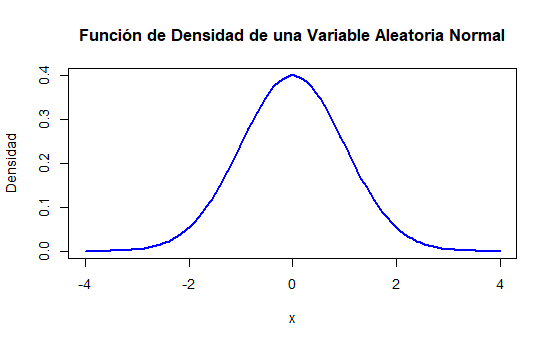
\includegraphics[width=10.6cm,height=\textheight,keepaspectratio]{normal.png}

}

\caption{Gráfica de una variable aleatoria normal}

\end{figure}%

\end{definition}

\begin{definition}[Variable aleatoria
Weibull]\protect\hypertarget{def-var_ale_weibull}{}\label{def-var_ale_weibull}

La variable aleatoria de Weibull es una variable continua utilizada
principalmente en estudios de confiabilidad y análisis de supervivencia
para modelar tiempos hasta un evento, como el tiempo de falla de un
sistema o la vida útil de un producto. La distribución de Weibull es
particularmente flexible y se puede ajustar a diferentes formas de datos
mediante sus dos parámetros: el parámetro de forma \((k)\) y el
parámetro de escala \((\lambda)\).

La función de densidad de probabilidad (PDF) para una variable aleatoria
\(X\) que sigue una distribución Weibull está definida como:

\[f(x; k, \lambda) = \begin{cases} \frac{k}{\lambda} \left( \frac{x}{\lambda} \right)^{k-1} e^{-(x/\lambda)^k} & x \geq 0, \\ 0 & x < 0, \end{cases}\]

donde:

\begin{itemize}
\item
  \(k>0\) : parámetro de forma que determina la forma de la
  distribución.

  \begin{itemize}
  \item
    Si \(k<1\), la función de probabilidad decrece con \(x\).
  \item
    Si \(k= 1\), la distribución se reduce a una exponencial.
  \item
    Si \(k > 1\), la función aumenta inicialmente, alcanza un máximo y
    luego decrece.
  \end{itemize}
\item
  \(\lambda > 0\): parámetro de escala que estira o comprime la
  distribución.
\end{itemize}

\end{definition}

\section{Valor esperado y varianza de una variable
aleatoria.}\label{valor-esperado-y-varianza-de-una-variable-aleatoria.}

\begin{definition}[Valor
esperado]\protect\hypertarget{def-valor_esperado}{}\label{def-valor_esperado}

Sean \(X\) una variable aleatoria real
(Definición~\ref{def-variable_aleatoria}) definida sobre el espacio de
probabilidad \((\Omega, \mathfrak{F}, P)\) .

\begin{enumerate}
\def\labelenumi{\arabic{enumi}.}
\tightlist
\item
  Si \(X\) es una variable aleatoria discreta, con valores
  \(x_1, x_2, \dots,\) se dice que \(X\) posee un valor esperado si:\\
  \[\sum_{k=1}^{\infty} |x_k| P(X = x_k) < \infty.\]
\end{enumerate}

En tal caso, se define el valor esperado \(E[X]\) (esperanza matemática
media) de \(X\) como: \[E[X] = \sum_{k=1}^{\infty} x_k P(X = x_k).\]

\begin{enumerate}
\def\labelenumi{\arabic{enumi}.}
\setcounter{enumi}{1}
\item
  Si \(X\) es una variable aleatoria continua con función de densidad
  \(f_x\), se dice que \(X\) posee un valor esperado si
  \[\int_{-\infty}^{\infty} |x| f_X(x)dx < \infty.\]

  En tal caso, se define el valor esperado \(E[X]\) (esperanza
  matemática media) de \(X\) como:
  \[E[X] = \int_{-\infty}^{\infty} xf_X(x) dx.\]
\end{enumerate}

\end{definition}

\begin{tcolorbox}[enhanced jigsaw, titlerule=0mm, opacityback=0, coltitle=black, bottomrule=.15mm, colbacktitle=quarto-callout-caution-color!10!white, toprule=.15mm, colback=white, arc=.35mm, colframe=quarto-callout-caution-color-frame, leftrule=.75mm, bottomtitle=1mm, left=2mm, toptitle=1mm, opacitybacktitle=0.6, breakable, title={Ejemplo (\textbf{\emph{Valor Esperado}})}, rightrule=.15mm]

Se lanza una moneda justa. Sea \(X\) la variable aleatoria que denota el
resultado obtenido, \(1\) si se obtiene cara y \(0\) si se obtiene cruz.

Para una moneda justa se tiene que \(P(cara)= \frac{1}{2}\) y
\(P(cruz)=\frac{1}{2}\).

El valor esperado \(E[X]\) es:

\[
E(X) = \sum(x_i \cdot P(x_i)) = 1\cdot \frac{1}{2} + 0 \cdot \frac{1}{2} = \frac{1}{2}
\]

\end{tcolorbox}

\begin{definition}[Varianza]\protect\hypertarget{def-varianza}{}\label{def-varianza}

Sea \(X\) una variable aleatoria con media \(\mu\), entonces la varianza
de \(X\), esta denotada por \(Var(X)\), se define como:
\[Var(X) = E[(X - \mu)^2].\]

\end{definition}

\begin{tcolorbox}[enhanced jigsaw, titlerule=0mm, opacityback=0, coltitle=black, bottomrule=.15mm, colbacktitle=quarto-callout-caution-color!10!white, toprule=.15mm, colback=white, arc=.35mm, colframe=quarto-callout-caution-color-frame, leftrule=.75mm, bottomtitle=1mm, left=2mm, toptitle=1mm, opacitybacktitle=0.6, breakable, title={Ejemplo (\textbf{\emph{Varianza}})}, rightrule=.15mm]

Supongase que se tiene una variable aleatoria \(X\) que toma los
siguientes valores con las respectivas probabilidades:

\begin{longtable}[]{@{}lllll@{}}
\toprule\noalign{}
\(X\) & \(1\) & \(2\) & \(3\) & \(4\) \\
\midrule\noalign{}
\endhead
\bottomrule\noalign{}
\endlastfoot
\(P(X)\) & \(0.1\) & \(0.3\) & \(0.4\) & \(0.2\) \\
\end{longtable}

Entonces \(\mu\) de \(X\) es:

\[
\mu = \sum_i x_iP(X = x_i) = 1(1.01) + 2(0.3) + 3(0.4)+ 4(0.2) = 2.7
\] Por lo que la varianza nos da:

\[
Var(X) = E[(X - \mu)^2] = \sum_{i}(x_i - \mu)^2 P(X= x_i)
\]

\[
Var(X) = (1- 2.7)^2(0.1) + (2- 2.7)^2(0.3) + (3- 2.7)^2(0.4) + (4- 2.7)^2(0.2) = 0.81
\]

Por lo tanto la varianza de \(X\) es \(Var(X) = 0.81\).

\end{tcolorbox}

\begin{definition}[Función generadora de
momentos]\protect\hypertarget{def-fun_gen_mom}{}\label{def-fun_gen_mom}

Sean \(X\) una variable aleatoria tal que \(E[e^{tx}]\) es finito para
todo \(t \in (-\alpha, \alpha)\), con \(\alpha\) real positivo. Se
define la función generadora de momentos de \(X\), denotada por
\(m_X(\cdot)\) como:
\[m_X(t) = E[e^{tX}]; \ \ con \  t \in (-\alpha, \alpha).\] Esto es:
\[f_X(x) = \left\{ \begin{array}{lcc} \sum_{k} e^{tx_{k}}P(X = x_k), & \text{si $X$ es una v.a discreta con valores $x = x_1, x_2\dotsb$} \\ \\ \int_{-\infty}^{\infty} e^{tx}f(x)dx, & \text{si $X$ es una v.a continua con función de densidad $f$.} \end{array} \right.\]

\end{definition}

\begin{tcolorbox}[enhanced jigsaw, titlerule=0mm, opacityback=0, coltitle=black, bottomrule=.15mm, colbacktitle=quarto-callout-caution-color!10!white, toprule=.15mm, colback=white, arc=.35mm, colframe=quarto-callout-caution-color-frame, leftrule=.75mm, bottomtitle=1mm, left=2mm, toptitle=1mm, opacitybacktitle=0.6, breakable, title={Ejemplo (\textbf{\emph{Función generadora de momentos}})}, rightrule=.15mm]

Se considera una variable aleatoria \(X\) que sigue una distribución
exponencial con parámetros \(\lambda\) y con función de densidad de
probabilidad : \(f_X(x) = \lambda e^{-\lambda x}, \ x \geq 0\).

La función generadora de momentos de \(X\) es:

\[
m_X(t) = E[e^{tX}] = \int_0^{\infty} e^{tx}\lambda e^{-\lambda x} dx = \lambda \int_0^{\infty} e^{x(t-\lambda)} dx.
\]La integral converge solo si \(t < \lambda\), y resolviendo queda como

\(m_X(t) = \lambda \left[\frac{e^{x(t - \lambda)}}{t - \lambda}\right]_{0}^{\infty} = \frac{\lambda}{\lambda - t}, \quad \text{para } t < \lambda.\)

\end{tcolorbox}

\section{Probabilidad condicional e
independencia}\label{sec-probabilidad-condicional-e-independencia}

La probabilidad condicional es un concepto fundamental en la teoría de
probabilidad. Se refiere a la probabilidad de que ocurra un evento
\(A\), dado que ya ha ocurrido otro evento \(B\).

\begin{definition}[Probabilidad
condicional]\protect\hypertarget{def-prob_cond}{}\label{def-prob_cond}

Sea \((\Omega, \mathfrak{F}, P)\) un espacio de probabilidad. Si
\(A, B, \in \mathfrak{F}\) con \(P(A) > 0\), entonces se define la
probabilidad del evento \(B\) bajo la condición \(A\) como sigue:
\[P(B | A) := \frac{P(A \cap B)}{P(A)}.\]

\end{definition}

\begin{tcolorbox}[enhanced jigsaw, titlerule=0mm, opacityback=0, coltitle=black, bottomrule=.15mm, colbacktitle=quarto-callout-caution-color!10!white, toprule=.15mm, colback=white, arc=.35mm, colframe=quarto-callout-caution-color-frame, leftrule=.75mm, bottomtitle=1mm, left=2mm, toptitle=1mm, opacitybacktitle=0.6, breakable, title={Ejemplo (\textbf{\emph{Probabilidad Condicional}})}, rightrule=.15mm]

Se lanzan dos dados. La probabilidad de que la suma de los dos dados sea
\(8\), dado que el primer dado ha mostrado un número mayor que \(3\) es
la siguiente.

\textbf{Solución:}

\begin{enumerate}
\def\labelenumi{\arabic{enumi}.}
\item
  Evento A: La suma de los dados es \(8\).
\item
  Evento B: El primer dado muestra un número mayor que \(3\).
\end{enumerate}

Primero se busca la \(P(B)\), es decir el primer dado puede mostrar
\(4, 5,\) o \(6\), lo que son 3 opciones de \(6\), por lo tanto:

\[
P(B) = \frac{3}{6} = \frac{1}{2}.
\]

Ahora para \(P(A \cap B)\), tenemos que es la probabilidad de que la
suma sea \(8\) y el primer dado mayor que \(3\). Las combinaciones que
cumplen con esto son: \((4,4), (5,3),(6,2)\), por lo que hay 3 casos
favorables de un total de 36 posibles., siendo así:

\[
P(A\cap B) = \frac{3}{36} = \frac{1}{12}.
\] Teniendo finalmente la probabilidad condicional:

\[
P(A|B) = \frac{\frac{1}{12}}{\frac{1}{2}} = \frac{2}{12} =\frac{1}{6}.
\]

\end{tcolorbox}

\begin{theorem}[Teorema de probabilidad
total]\protect\hypertarget{thm-prob_total}{}\label{thm-prob_total}

Sea \(A_1, A_2, ...\) una partición finita o numerable de \(\Omega\), es
decir, \(A_i \cap A_j = \emptyset\) \emph{para todo} \(i\neq j\)
\emph{y} \(\bigcup_{i=1}^{\infty} A_i = \Omega\) tal que \(P(A_i)>0\)
\emph{para todo} \(i\)\emph{. Entonces para cualquier}
\(B \in \mathfrak{F}\) \emph{se satisface:}

\[
P(B) = \sum_n P(B|A_n)P(A_n).
\]

\end{theorem}

La demostración del Teorema~\ref{thm-prob_total} puede ser consultado en
\autocite{castaneda2012introduction}.

En algunos casos la ocurrencia de un evento no afecta la probabilidad de
ocurrencia de otro evento. En ese caso se dice que el primer evento es
independiente del otro.

\begin{definition}[Eventos
independientes]\protect\hypertarget{def-even_ind}{}\label{def-even_ind}

Dos eventos son independientes \(A\) y \(B\) son independientes, si y
solo si, \[P(A \cap B) = P(A)P(B).\]En caso contrario se dice que los
eventos son dependientes.

\end{definition}

\begin{tcolorbox}[enhanced jigsaw, titlerule=0mm, opacityback=0, coltitle=black, bottomrule=.15mm, colbacktitle=quarto-callout-caution-color!10!white, toprule=.15mm, colback=white, arc=.35mm, colframe=quarto-callout-caution-color-frame, leftrule=.75mm, bottomtitle=1mm, left=2mm, toptitle=1mm, opacitybacktitle=0.6, breakable, title={Ejemplo (\textbf{\emph{Ejemplo de eventos independientes}})}, rightrule=.15mm]

Supongamos que lanzas dos monedas. Los eventos siguientes son
independientes:

\begin{itemize}
\item
  \textbf{Evento A}: \(\text{``La primera moneda muestra cara."}\)
\item
  \textbf{Evento B}: \(\text{``La segunda moneda muestra cara."}\)
\end{itemize}

La probabilidad de que el evento \(A\) ocurra es
\(P(A) = \frac{1}{2}\)\hspace{0pt} y la probabilidad de que el evento B
ocurra también es \(P(B) = \frac{1}{2}\)\hspace{0pt}. La probabilidad
conjunta de que ambos eventos ocurran es
\(P(A \cap B) = \frac{1}{2} \times \frac{1}{2} = \frac{1}{4}\) Como
\(P(A \cap B) = P(A) \cdot P(B)\), estos eventos son independientes.

\end{tcolorbox}

\section{Independencia de variables
aleatorias}\label{independencia-de-variables-aleatorias}

\begin{definition}[Independencia de variables
aleatorias]\protect\hypertarget{def-ind_var_ale}{}\label{def-ind_var_ale}

Las variables aleatorias \(X\) e \(Y\) son independientes si para dos
conjuntos cualesquiera de números reales \(A\) y \(B\),
\[P[X \in A, Y \in B] = P(\{\omega \in \Omega: X(\omega) \in A)P(\{\omega \in \Omega: X(\omega) \in B).\]

En otras palabras, \(X\) e \(Y\) son independientes si, para todos \(A\)
y \(B\), los eventos \(E_A = [X \in A]\) y \(F_B = [Y \in B]\) son
independientes.

\end{definition}

\section{Probabilidad condicional de una variable
aleatoria}\label{probabilidad-condicional-de-una-variable-aleatoria}

La probabilidad condicional de una variable aleatoria es la probabilidad
de que ocurra un evento, dado que otro evento ya ha ocurrido. En
resumen, la probabilidad condicional es crucial para entender cómo la
ocurrencia de un evento afecta la probabilidad de otro, lo que tiene
amplias aplicaciones en análisis de datos, estadística, y muchas otras
disciplinas.

\subsection{Valor esperado condicionado dada una variable
aleatoria}\label{valor-esperado-condicionado-dada-una-variable-aleatoria}

\begin{definition}[Valor esperado condicional de v. a.
discretas]\protect\hypertarget{def-val_es_cond_v_a}{}\label{def-val_es_cond_v_a}

El valor esperado condicional de \(X\) dado \(Y = y\) se define así:
\[E[X | Y = y] =: \sum_x xf_{X|Y}(x | y),\] para todos los \(y\) para
los cuales \(P(Y = y) > 0\).

\end{definition}

\subsection{Varianza condicionada dada una variable
aleatoria}\label{varianza-condicionada-dada-una-variable-aleatoria}

\begin{definition}[Varianza condicionada dada una variable
aleatoria]\protect\hypertarget{def-vari_cond_var_ale}{}\label{def-vari_cond_var_ale}

Si \(X\) y \(Y\) son dos variables aleatorias, la varianza condicionada
de \(X\) dado \(Y=y\) se denota como \(Var(X | Y=Y)\) y se define como:
\[Var( X | Y = y) = E[(X - E[X|Y=y])^2 | Y = y].\]

Donde \(E[X |Y =y]\) es la esperanza condicional de \(X\) dado
\(Y = y\).

\end{definition}

\begin{definition}[Convolución]\protect\hypertarget{def-convolucion}{}\label{def-convolucion}

Para dos medidas \(\sigma\) -finitas cualesquiera \(\mu\) y \(\lambda\)
en \((\mathbb{R}, \mathcal{B}(\mathbb{R}))\), la medida
\((\mu*\lambda)(A)\) definida como:

\[
(\mu*\lambda)(A) \equiv \int \int I_A(x+y)\mu(dx)\lambda(dy),
\]

se denomina convolución de \(\mu\) y \(\lambda\).

\end{definition}

\section{Ley fuerte de los grandes
números}\label{ley-fuerte-de-los-grandes-nuxfameros}

La ley fuerte de los grandes números es probablemente el resultado más
conocido de la teoría de la probabilidad. Establece que el promedio de
una secuencia de variables aleatorias independientes que tengan una
distribución común, con probabilidad \(1\), convergerán a la media de
esa distribución.

\begin{theorem}[Ley fuerte de los grandes
números]\protect\hypertarget{thm-ley_f_gran_num}{}\label{thm-ley_f_gran_num}

Sea \(X_1, X_2, ...\) una secuencia de variables aleatorias
independientes e idénticamente distribuidas, cada una de las cuales
tiene media finita \(\mu = E[X_i]\). Entonces con probabilidad \(1\) se
tiene que:

\[ \frac{X_1 + X_2 + \dots + X_n}{n} \rightarrow \mu \qquad \text{cuando $n \rightarrow \infty^{\uparrow}$} \]

\end{theorem}

La demostración del Teorema~\ref{thm-ley_f_gran_num} puede ser
consultado en \autocite{ross2015first}.

\chapter{Estadística}\label{estaduxedstica}

La estadística es una disciplina matemática que se encarga de recopilar,
analizar e interpretar datos para extraer conclusiones útiles y tomar
decisiones informadas. Su origen se remonta a la antigüedad, donde
civilizaciones como la egipcia y la babilónica ya utilizaban registros
numéricos para fines administrativos y de organización. Sin embargo, el
desarrollo formal de la estadística como ciencia comenzó en el siglo
XVII con la obra de matemáticos como John Graunt, quien analizó los
registros de mortalidad en Londres, y Pierre-Simon Laplace, que
desarrolló técnicas probabilísticas.

La estadística se divide en dos grandes ramas: la estadística
descriptiva y la inferencial. La estadística descriptiva se centra en
resumir y describir las características de un conjunto de datos a través
de medidas como la media, la mediana, la moda, y la desviación estándar,
al igual que mediante representaciones gráficas como histogramas y
diagramas de dispersión. Por otro lado, la estadística inferencial
utiliza técnicas de muestreo y probabilidad para hacer generalizaciones
y predicciones sobre una población a partir de una muestra de datos.

En la vida diaria, la estadística tiene numerosas aplicaciones. Por
ejemplo, en la medicina, se utiliza para evaluar la eficacia de nuevos
tratamientos mediante ensayos clínicos y para estudiar la incidencia de
enfermedades. En el ámbito económico, ayuda a analizar tendencias del
mercado, prever el comportamiento de los consumidores y tomar decisiones
financieras. En la educación, se emplea para evaluar el rendimiento
académico y diseñar políticas educativas. Además, la estadística es
fundamental en la investigación científica para validar hipótesis y
teorías a través del análisis de datos experimentales.

Para brindar más información (\autocite{walpole2012probabilidad},
\autocite{jones1994book},\autocite{massey1951kolmogorov},
\autocite{wackerly2009estadística}, \autocite{mood1986introduction})
presentan las siguientes definiciones.

\begin{definition}[Estadístico]\protect\hypertarget{def-estadis}{}\label{def-estadis}

Un estadístico es una función de variables aleatorias observables que no
contienen parámetros desconocidos.

\end{definition}

\begin{definition}[Muestra
aleatoria]\protect\hypertarget{def-muestra_aleatoria}{}\label{def-muestra_aleatoria}

Sean \(x_1, x_2, ..., x_n\) variables aleatorias cuya distribución
conjunta es

\[
g(x_1, x_2, ..., x_n) = f(x_1) f(x_2)\dotsb f(x_n)
\]

donde la función de densidad de cada \(x_i\) es \(f(x)\). En tal
supuesto se dice que \(x_1, x_2, ..., x_n\) es una muestra aleatoria de
tamaño \(n\) de la población con densidad \(f(x)\).

\end{definition}

\section{Medidas de localización}\label{medidas-de-localizaciuxf3n}

Las medidas de localización son estadísticas que resumen o describen la
tendencia central de un conjunto de datos. Las más comunes incluyen la
media y mediana. Estas medidas ayudan a identificar el valor central o
típico de los datos, proporcionando una referencia útil para entender su
distribución y comportamiento. Las medidas de localización son
fundamentales en estadística porque proporcionan un resumen rápido de la
distribución de los datos. Ayudan a comparar datos, tomar decisiones y
entender la distribución.

\begin{definition}[Media
muestral]\protect\hypertarget{def-media}{}\label{def-media}

El primer momento de la muestra es la \emph{media muestral}, definida
como

\[\bar{X} = \frac{1}{n} \sum_{i=1}^n X_i.\]

\end{definition}

La mediana de la muestra es una medida de tendencia central que divide
los datos en dos partes iguales, la mitad por debajo de la mediana y la
otra mitad por encima. Si el número de observaciones es uniforme, la
mediana está a medio camino entre los dos valores centrales

\begin{definition}[Mediana]\protect\hypertarget{def-mediana}{}\label{def-mediana}

Dado que las observaciones en una muestra son \(x_1, x_2, \cdots x_n\)
acomodadas en orden de magnitud creciente, la mediana de la muestra es

\[
\bar{X} = \left\{ \begin{array}{lcc} x_{\frac{n+1}{2}}, & \text{si $n$ es impar}, \\ \\ \frac{1}{2}(x_{\frac{n}{2}} + x_{\frac{n}{2}+1}), & \text{si $n$ es par}. \end{array} \right.
\]

\end{definition}

\section{Elementos de teoría de
muestreo}\label{elementos-de-teoruxeda-de-muestreo}

La teoría de muestreo es una rama de la estadística que se ocupa del
diseño y análisis de muestras. La teoría de muestreo es crucial porque
permite inferir características de una población a partir de una muestra
representativa. Esto es esencial en estudios donde es impracticable o
imposible examinar a toda la población debido a limitaciones de tiempo,
costos o logística. Un muestreo adecuado asegura que las inferencias
hechas sobre la población sean precisas y confiables, minimizando el
error de muestreo y permitiendo un análisis eficiente.

\subsection{Población}\label{poblaciuxf3n}

\begin{definition}[]\protect\hypertarget{def-poblacion}{}\label{def-poblacion}

Es el conjunto completo de elementos o individuos que se desean
estudiar. Puede ser finita o infinita.

\end{definition}

\begin{itemize}
\tightlist
\item
  Ejemplo: Todos los estudiantes de una universidad.
\end{itemize}

\subsection{Muestra}\label{muestra}

\begin{definition}[]\protect\hypertarget{def-muestra}{}\label{def-muestra}

Subconjunto de la población seleccionado para el estudio. Una muestra
debe ser representativa para que las inferencias realizadas a partir de
ella sean válidas para la población total.

\begin{itemize}
\tightlist
\item
  Ejemplo: Un grupo de 200 estudiantes seleccionados aleatoriamente de
  la universidad.
\end{itemize}

\end{definition}

\subsection{Unidad de Muestreo}\label{unidad-de-muestreo}

\begin{definition}[]\protect\hypertarget{def-unidad_muestreo}{}\label{def-unidad_muestreo}

Cada uno de los elementos individuales que componen la muestra. Es la
unidad básica sobre la cual se toman las mediciones.

\end{definition}

\begin{itemize}
\tightlist
\item
  Ejemplo: Un estudiante específico en el grupo de 200 estudiantes.
\end{itemize}

\subsection{Marco Muestral}\label{marco-muestral}

\begin{definition}[]\protect\hypertarget{def-muestral}{}\label{def-muestral}

Lista completa de todas las unidades de muestreo en la población de
donde se seleccionará la muestra. Debe ser exhaustivo y actualizado para
minimizar sesgos.

\end{definition}

\begin{itemize}
\tightlist
\item
  Ejemplo: Lista de todos los estudiantes matriculados en la
  universidad.
\end{itemize}

\subsection{Parámetro}\label{paruxe1metro}

\begin{definition}[]\protect\hypertarget{def-parámetro}{}\label{def-parámetro}

Característica numérica de la población que se desea estimar, como la
media, proporción o varianza.

\end{definition}

\begin{itemize}
\tightlist
\item
  Ejemplo: La media de la calificación final de todos los estudiantes de
  la universidad.
\end{itemize}

\subsection{Estadístico}\label{estaduxedstico-1}

\begin{definition}[]\protect\hypertarget{def-estadistico}{}\label{def-estadistico}

Valor calculado a partir de los datos de la muestra, utilizado para
estimar el parámetro poblacional.

\end{definition}

\begin{itemize}
\tightlist
\item
  Ejemplo: La media de la calificación final de los 200 estudiantes
  seleccionados.
\end{itemize}

\subsection{Error de Muestreo}\label{error-de-muestreo}

\begin{definition}[]\protect\hypertarget{def-error_muestreo}{}\label{def-error_muestreo}

Diferencia entre el valor del parámetro poblacional y el estadístico de
la muestra. Es un error inherente que surge porque se está trabajando
con una muestra en lugar de toda la población.

\end{definition}

\begin{itemize}
\tightlist
\item
  Ejemplo: Diferencia entre la media de la calificación final de todos
  los estudiantes y la media obtenida de los 200 estudiantes
  seleccionados.
\end{itemize}

\subsection{Técnicas de Muestreo}\label{tuxe9cnicas-de-muestreo}

\begin{definition}[]\protect\hypertarget{def-tecnicas_muestreo}{}\label{def-tecnicas_muestreo}

Métodos utilizados para seleccionar una muestra de la población.
Incluyen muestreo aleatorio simple, muestreo estratificado, muestreo por
conglomerados, entre otros.

\end{definition}

\begin{itemize}
\tightlist
\item
  Ejemplo: En el muestreo aleatorio simple, cada estudiante tiene la
  misma probabilidad de ser seleccionado.
\end{itemize}

\subsection{Importancia de la Teoría de
Muestreo}\label{importancia-de-la-teoruxeda-de-muestreo}

La teoría de muestreo es crucial porque permite hacer inferencias sobre
una población sin necesidad de examinar a cada miembro. Esto es esencial
en la investigación en ciencias sociales, biología, marketing, y muchos
otros campos donde examinar toda la población sería costoso o
impracticable.

\section{Gráficos estadísticos}\label{gruxe1ficos-estaduxedsticos}

\subsection{Histograma}\label{sec-histogramas}

Un histograma es un tipo de gráfico utilizado en estadística para
representar la distribución de una variable cuantitativa continua. Se
construye dividiendo el rango de datos en intervalos (también conocidos
como ``bins'' o clases), y luego contando el número de observaciones que
caen dentro de cada intervalo.

Cada intervalo se representa como una barra rectangular, donde la altura
de la barra es proporcional a la frecuencia (número de observaciones) o
a la densidad (frecuencia relativa) de los datos en ese intervalo. A
diferencia de un gráfico de barras, las barras en un histograma están
unidas entre sí, lo que refleja la continuidad de los datos.

\subsection{Componentes de un
Histograma}\label{componentes-de-un-histograma}

\begin{enumerate}
\def\labelenumi{\arabic{enumi}.}
\item
  Intervalos o Bins: Divisiones del rango de datos en segmentos de igual
  ancho. El número y el ancho de los intervalos pueden afectar la
  apariencia del histograma.
\item
  Frecuencia: Número de observaciones que caen dentro de cada intervalo.
  Se puede representar como frecuencia absoluta (conteo) o como
  frecuencia relativa (porcentaje).
\item
  Barras: Rectángulos cuya altura corresponde a la frecuencia de las
  observaciones en cada intervalo.
\end{enumerate}

\subsection{Box Plot}\label{sec-boxplot}

Un boxplot (o diagrama de caja y bigotes) es un gráfico estadístico que
resume la distribución de un conjunto de datos numéricos a través de
cinco estadísticos clave: el mínimo, el primer cuartil \((Q1)\), la
mediana \((Q2)\), el tercer cuartil \((Q3)\), y el máximo. Este tipo de
gráfico es especialmente útil para identificar la dispersión, la
asimetría, y los valores atípicos (outliers) en un conjunto de datos.

\subsection{Componentes de un Boxplot}\label{componentes-de-un-boxplot}

\begin{enumerate}
\def\labelenumi{\arabic{enumi}.}
\item
  Caja (Box):

  \begin{itemize}
  \item
    Primer cuartil \((Q1)\): Marca el límite inferior de la caja,
    representando el \(25\%\) de los datos por debajo de este valor.
  \item
    Mediana \((Q2)\): Línea dentro de la caja que representa el valor
    medio (\(50\%\) de los datos están por debajo y \(50\%\) por
    encima).
  \item
    Tercer cuartil \((Q3)\): Marca el límite superior de la caja,
    representando el \(75\%\) de los datos por debajo de este valor.
  \item
    Rango intercuartílico (IQR): Es la longitud de la caja, calculada
    como \(Q3\) - \(Q1\). Mide la dispersión central del conjunto de
    datos.
  \end{itemize}
\item
  Bigotes (Whiskers):

  \begin{itemize}
  \item
    Se extienden desde los extremos de la caja hasta el valor mínimo y
    máximo dentro de \(1.5\) veces el rango intercuartílico (IQR) desde
    el primer y tercer cuartil, respectivamente.
  \item
    Los valores que caen fuera de estos límites se consideran valores
    atípicos.
  \end{itemize}
\item
  Valores Atípicos (Outliers):

  \begin{itemize}
  \tightlist
  \item
    Son los puntos de datos que se encuentran fuera del rango cubierto
    por los bigotes. Se representan como puntos individuales o pequeños
    círculos fuera de la caja y los bigotes.
  \end{itemize}
\end{enumerate}

\subsection{Propósito del Boxplot}\label{propuxf3sito-del-boxplot}

El boxplot se utiliza principalmente para:

\begin{itemize}
\item
  Visualizar la distribución: Permite ver de manera rápida la
  distribución de los datos, su simetría o asimetría, y la presencia de
  valores atípicos.
\item
  Comparar distribuciones: Es útil para comparar la distribución de
  datos entre diferentes grupos o categorías.
\item
  Identificar valores atípicos: Facilita la detección de outliers que
  pueden influir significativamente en el análisis.
\end{itemize}

\begin{center}
\pandocbounded{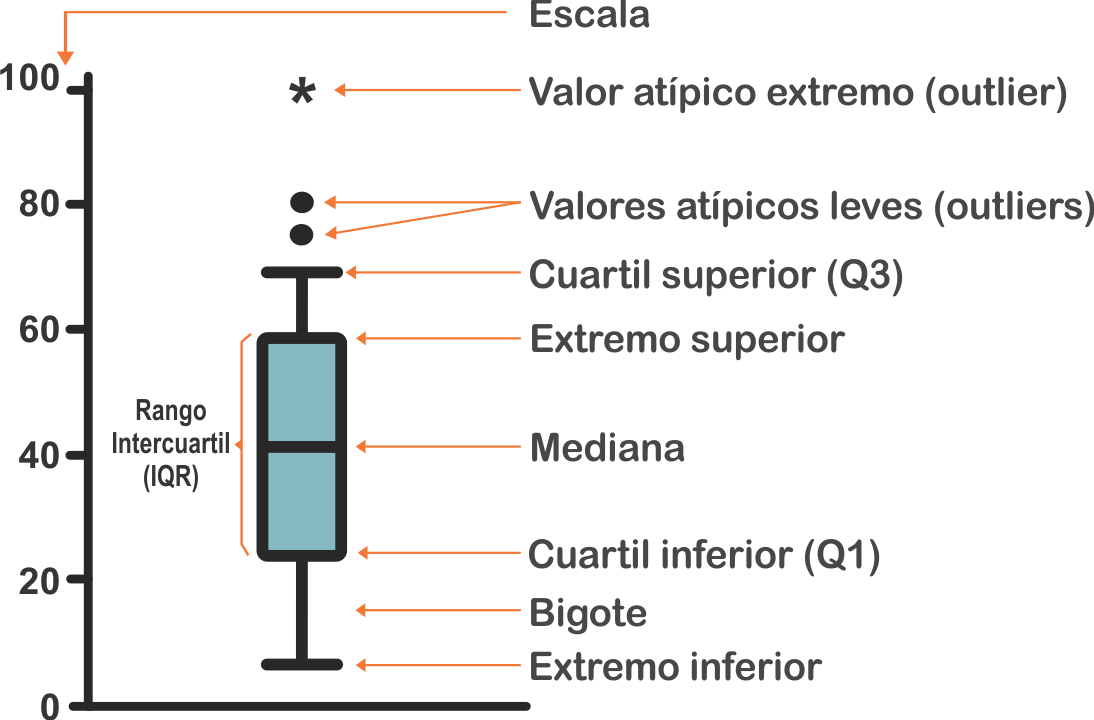
\includegraphics[keepaspectratio]{box2.png}}
\end{center}

\section{Pruebas de hipótesis.}\label{pruebas-de-hipuxf3tesis.}

Las pruebas de hipótesis son un conjunto de procedimientos estadísticos
utilizados para tomar decisiones sobre una población basándose en la
información obtenida de una muestra. El propósito principal de estas
pruebas es determinar si existe suficiente evidencia en los datos
muéstrales para rechazar una hipótesis nula \((H_0)\) en favor de una
hipótesis alternativa \((H_1)\).

\begin{definition}[]\protect\hypertarget{def-hip_est}{}\label{def-hip_est}

Una hipótesis estadística es una aseveración o conjetura respecto a una
o más poblaciones.

\end{definition}

\subsection{Conceptos Clave en Pruebas de
Hipótesis}\label{conceptos-clave-en-pruebas-de-hipuxf3tesis}

\begin{enumerate}
\def\labelenumi{\arabic{enumi}.}
\item
  Hipótesis Nula \(H_o\):

  \begin{itemize}
  \item
    Es una afirmación que se plantea inicialmente y que se somete a
    prueba. Generalmente, representa una situación de ``no efecto'' o
    ``no diferencia''.
  \item
    Ejemplo: ``La media de la población es igual a \(50\)''.
  \end{itemize}
\item
  Hipótesis Alternativa \(H_a\) o \(H_1\) :

  \begin{itemize}
  \item
    Es la afirmación que se acepta si la evidencia contra \(H_0\) es
    suficiente. Representa una situación de ``efecto'' o ``diferencia''.
  \item
    Ejemplo: ``La media de la población es diferente de \(50\)''.
  \end{itemize}
\item
  Estadístico de Prueba:

  \begin{itemize}
  \tightlist
  \item
    Es un valor calculado a partir de los datos muéstrales que se
    utiliza para decidir si se rechaza o no la hipótesis nula. Este
    valor se compara con una distribución de referencia (normal, \(t\)
    de Student, chi-cuadrado, etc.) para determinar la significancia.
  \end{itemize}
\item
  Nivel de Significancia (\(\alpha\)):

  \begin{itemize}
  \item
    Es la probabilidad de rechazar la hipótesis nula cuando en realidad
    es verdadera (error tipo I). Comúnmente se elige un valor de
    \(\alpha= 0.05\), aunque puede variar dependiendo del contexto del
    estudio.
  \item
    Ejemplo: Un nivel de significancia de \(0.05\) significa que hay un
    \(5\%\) de probabilidad de cometer un error tipo I.
  \end{itemize}
\item
  Valor-p (p-value):

  \begin{itemize}
  \item
    Es la probabilidad de obtener un resultado tan extremo como el
    observado en los datos muéstrales, asumiendo que la hipótesis nula
    es verdadera. Si el valor-p es menor que \(\alpha\), se rechaza
    \(H_0\).
  \item
    Ejemplo: Un valor-p de \(0.03\) indica que hay un \(3 \%\) de
    probabilidad de obtener los datos observados si la hipótesis nula es
    verdadera.
  \end{itemize}
\item
  Decisión:

  \begin{itemize}
  \item
    Rechazar \(H_0\): Si el valor-p es menor que \(\alpha\) se concluye
    que hay suficiente evidencia para rechazar la hipótesis nula a favor
    de la alternativa.
  \item
    No Rechazar \(H_0\): Si el valor-p es mayor que \(\alpha\), no se
    rechaza la hipótesis nula, lo que no implica que sea verdadera, sino
    que no hay suficiente evidencia en contra.
  \end{itemize}
\end{enumerate}

\section{Test de normalidad.}\label{sec-normalidad}

Un test de normalidad es una prueba estadística que se utiliza para
determinar si un conjunto de datos sigue una distribución normal. La
normalidad es un supuesto clave en muchas pruebas estadísticas, como la
prueba \(t\) de Student y el análisis de varianza (ANOVA), porque muchas
inferencias estadísticas asumen que los datos son aproximadamente
normales. Si los datos no siguen una distribución normal, algunos
métodos estadísticos pueden no ser válidos o pueden ofrecer resultados
engañosos.

\subsection{Propósito}\label{propuxf3sito}

El propósito principal de un test de normalidad es evaluar si la muestra
de datos tiene una distribución que sea aproximadamente simétrica y con
una forma de campana, como lo haría una distribución normal. Existen
varios test de normalidad, y cada uno tiene su propio enfoque para medir
esta adecuación.

\subsection{Principales tipos de tests de
normalidad}\label{principales-tipos-de-tests-de-normalidad}

\begin{enumerate}
\def\labelenumi{\arabic{enumi}.}
\item
  Prueba de Kolmogorov-Smirnov (K-S): Este test compara la distribución
  empírica de los datos con una distribución normal teórica, midiendo la
  distancia máxima entre ambas distribuciones.
\item
  Prueba de Shapiro-Wilk: Considerada una de las pruebas más poderosas,
  especialmente en pequeñas muestras, evalúa la normalidad calculando
  una estadística basada en las correlaciones entre los datos y sus
  posiciones esperadas bajo una distribución normal.
\item
  Prueba de Anderson-Darling: Similar a la K-S, pero con más peso en las
  colas de la distribución, lo que la hace más sensible a los valores
  atípicos.
\item
  Prueba de Jarque-Bera: Evalúa la normalidad basándose en la asimetría
  (skewness) y la curtosis de los datos. Es útil cuando los datos tienen
  distribuciones que se desvían significativamente de la normal.
\end{enumerate}

\section{Jarque Bera}\label{sec-J_B}

\subsection{Test de Jarque-Bera: Definición y
Uso}\label{test-de-jarque-bera-definiciuxf3n-y-uso}

El Test de Jarque-Bera (JB) es una prueba estadística utilizada para
evaluar si una serie de datos sigue una distribución normal.
Específicamente, se basa en las diferencias de la curtosis y la
asimetría (skewness) de la muestra con respecto a las de una
distribución normal.

\subsection{Conceptos Clave}\label{conceptos-clave}

\begin{enumerate}
\def\labelenumi{\arabic{enumi}.}
\item
  Asimetría (Skewness):

  \begin{itemize}
  \item
    Mide la simetría de la distribución de los datos. Una distribución
    normal tiene una asimetría de 0.
  \item
    La asimetría positiva indica que la cola derecha es más larga,
    mientras que la asimetría negativa indica que la cola izquierda es
    más larga.
  \end{itemize}
\item
  Curtosis:

  \begin{itemize}
  \item
    Mide la ``concentración'' de los datos en torno a la media. Una
    distribución normal tiene una curtosis de 3.
  \item
    La curtosis mayor que 3 (leptocúrtica) indica una distribución con
    colas más largas, mientras que una curtosis menor que 3
    (platicúrtica) indica una distribución con colas más cortas.
  \end{itemize}
\item
  Estadístico de Jarque-Bera:

  \begin{itemize}
  \item
    Se calcula a partir de la asimetría (S) y la curtosis (K) de la
    muestra mediante la fórmula:

    \[JB = \frac{n}{6} \left( S^2 + \frac{(K - 3)^2}{4} \right).\]
  \end{itemize}

  Donde \(n\) es el tamaño de la muestra, \(S\) es la asimetría y \(K\)
  es la curtosis.
\item
  Hipótesis:

  \begin{itemize}
  \item
    Hipótesis nula (H₀): Los datos siguen una distribución normal.
  \item
    Hipótesis alternativa (H₁): Los datos no siguen una distribución
    normal.
  \end{itemize}
\item
  Valor Crítico y Decisión:

  \begin{itemize}
  \tightlist
  \item
    El estadístico JB se compara con un valor crítico de la distribución
    chi-cuadrado con dos grados de libertad. Si el valor del estadístico
    es mayor que el valor crítico o si el valor-p asociado es menor que
    el nivel de significancia (\(\alpha\)), se rechaza la hipótesis
    nula, indicando que los datos no siguen una distribución normal.
  \end{itemize}
\end{enumerate}

\section{Kolmogorov Smirnov}\label{sec-K_S}

El Test de Kolmogorov-Smirnov (K-S) es una prueba no paramétrica
utilizada para determinar si una muestra de datos sigue una distribución
teórica específica (por ejemplo, normal, exponencial, etc.) o para
comparar dos muestras para verificar si provienen de la misma
distribución. Es especialmente útil porque no requiere que la
distribución subyacente de los datos sea normal, lo que lo hace
aplicable en una amplia variedad de situaciones.

\subsection{Conceptos Clave}\label{conceptos-clave-1}

\begin{enumerate}
\def\labelenumi{\arabic{enumi}.}
\item
  Función de Distribución Empírica (FDE):

  \begin{itemize}
  \tightlist
  \item
    Es una función que estima la distribución acumulativa de la muestra
    de datos. Se calcula como la proporción de puntos en la muestra que
    son menores o iguales a un valor dado.
  \end{itemize}
\item
  Función de Distribución Teórica:

  \begin{itemize}
  \tightlist
  \item
    Es la función de distribución acumulativa de la distribución que se
    está comparando con los datos (por ejemplo, la distribución normal,
    exponencial, etc.).
  \end{itemize}
\item
  Estadístico de Kolmogorov-Smirnov:

  \begin{itemize}
  \tightlist
  \item
    Es la máxima diferencia absoluta entre la función de distribución
    empírica de los datos y la función de distribución teórica:
  \end{itemize}

  \[D = \sup_x |F_n(x) - F(x)|.\]

  Donde \(F_n(x)\) es la función de distribución empírica de la muestra
  y \(F(x)\) es la función de distribución teórica.
\item
  Hipótesis:

  \begin{itemize}
  \item
    Hipótesis nula \((H_0)\): La muestra sigue la distribución teórica
    especificada.
  \item
    Hipótesis alternativa \((H_1)\): La muestra no sigue la distribución
    teórica especificada.
  \end{itemize}
\item
  Valor Crítico y Decisión:

  \begin{itemize}
  \tightlist
  \item
    El estadístico D se compara con un valor crítico basado en la
    distribución K-S. Si el estadístico D es mayor que el valor crítico,
    o si el valor-p es menor que el nivel de significancia (\(\alpha\)),
    se rechaza la hipótesis nula.
  \end{itemize}
\end{enumerate}

\subsection{Aplicaciones del Test de
Kolmogorov-Smirnov}\label{aplicaciones-del-test-de-kolmogorov-smirnov}

El Test de Kolmogorov-Smirnov se utiliza en muchas áreas, incluyendo la
econometría, biología, y análisis de datos. Es comúnmente empleado para
validar modelos estadísticos, verificar la normalidad de los datos, o
comparar distribuciones de diferentes muestras.

\subsection{Variantes del Test}\label{variantes-del-test}

\begin{enumerate}
\def\labelenumi{\arabic{enumi}.}
\item
  Test de Kolmogorov-Smirnov Bivariado: Compara dos muestras y evalúa si
  provienen de la misma distribución.
\item
  Test de Lilliefors: Una adaptación del test K-S para cuando se estima
  la media y la varianza de la distribución normal a partir de la
  muestra.
\end{enumerate}

\begin{tcolorbox}[enhanced jigsaw, titlerule=0mm, opacityback=0, coltitle=black, bottomrule=.15mm, colbacktitle=quarto-callout-caution-color!10!white, toprule=.15mm, colback=white, arc=.35mm, colframe=quarto-callout-caution-color-frame, leftrule=.75mm, bottomtitle=1mm, left=2mm, toptitle=1mm, opacitybacktitle=0.6, breakable, title={Ejemplo (\textbf{\emph{Test KS}})}, rightrule=.15mm]

Un \textbf{Q-Q plot} combinado con la \textbf{prueba de
Kolmogorov-Smirnov} (K-S) se utiliza para verificar si un conjunto de
datos sigue una distribución teórica específica (por ejemplo, una
normal).

\begin{enumerate}
\def\labelenumi{\arabic{enumi}.}
\tightlist
\item
  \textbf{Prueba de Kolmogorov-Smirnov (K-S)}:
\end{enumerate}

\begin{itemize}
\tightlist
\item
  \textbf{Objetivo:} Comparar la función de distribución acumulativa
  (FDA) empírica de los datos con la FDA de una distribución teórica.
\item
  \textbf{Hipótesis:}

  \begin{itemize}
  \tightlist
  \item
    \((H_0)\): Los datos siguen la distribución teórica.
  \item
    \((H_a)\): Los datos no siguen la distribución teórica.
  \end{itemize}
\item
  \textbf{Estadístico K-S ((D))}: Es la mayor diferencia absoluta entre
  la FDA empírica y la teórica.
\end{itemize}

\begin{enumerate}
\def\labelenumi{\arabic{enumi}.}
\setcounter{enumi}{1}
\item
  \textbf{Q-Q Plot}: El Q-Q plot es una representación gráfica que
  complementa la prueba K-S al comparar cuantiles de los datos con los
  cuantiles de una distribución teórica. Si los datos siguen la
  distribución teórica, los puntos deberían alinearse sobre la línea
  \((y = x)\).
\item
  Ejemplo de que ilustra cómo los datos se comparan con una distribución
  normal:

  \begin{center}
  \includegraphics[width=3.47917in,height=\textheight,keepaspectratio]{images/clipboard-3064661078.png}
  \end{center}
\end{enumerate}

\subsection{Descripción del
gráfico:}\label{descripciuxf3n-del-gruxe1fico}

\begin{enumerate}
\def\labelenumi{\arabic{enumi}.}
\tightlist
\item
  \textbf{Cuantiles teóricos vs.~muestrales:} Los puntos azules
  representan los datos muestrales en comparación con una distribución
  normal teórica.
\item
  \textbf{Línea de referencia} \((y=x)\)\textbf{:} Indica cómo deberían
  alinearse los puntos si los datos siguen la distribución teórica.
\item
  \textbf{Estadístico K-S:} La distancia vertical máxima ((D)) entre un
  punto de los datos y la línea de referencia se marca con una flecha
  roja.
\end{enumerate}

\end{tcolorbox}

\section{Monte Carlo}\label{sec-Mon_Car}

El Método de Monte Carlo es un conjunto de técnicas estadísticas que
utilizan simulaciones aleatorias para resolver problemas matemáticos y
físicos que son difíciles o imposibles de resolver de manera exacta
mediante métodos determinísticos. Este enfoque se basa en generar
múltiples muestras aleatorias para estimar una solución aproximada. Es
ampliamente utilizado en áreas como la física, las finanzas, la
ingeniería, la biología y otros campos donde la complejidad del problema
o la incertidumbre inherente hacen que otros métodos no sean prácticos.

Cuando se trabaja con variables aleatorias, comúnmente se quiere estimar
el valor esperado de cualquier cantidad.

\begin{tcolorbox}[enhanced jigsaw, titlerule=0mm, opacityback=0, coltitle=black, bottomrule=.15mm, colbacktitle=quarto-callout-caution-color!10!white, toprule=.15mm, colback=white, arc=.35mm, colframe=quarto-callout-caution-color-frame, leftrule=.75mm, bottomtitle=1mm, left=2mm, toptitle=1mm, opacitybacktitle=0.6, breakable, title={Ejemplo (\textbf{\emph{Monte Carlo}})}, rightrule=.15mm]

Este es un ejemplo de cómo generar una representación gráfica del método
de Monte Carlo, donde los puntos azules caen dentro del círculo y los
puntos rojos fuera de él.

\begin{center}
\includegraphics[width=3.21875in,height=\textheight,keepaspectratio]{images/clipboard-3088952609.png}
\end{center}

\subsection{Interpretación del
gráfico:}\label{interpretaciuxf3n-del-gruxe1fico}

\begin{itemize}
\tightlist
\item
  \textbf{Puntos dentro del círculo}: Representan los puntos aleatorios
  que están dentro de la región que se utiliza para estimar \((\pi)\).
\item
  \textbf{Puntos fuera del círculo}: Representan los puntos que no
  cumplen la condición de \((x^2 + y^2 \leq 1)\).
\end{itemize}

Este gráfico proporciona una visualización del proceso de simulación
utilizado en el método de Monte carlo para la estimación de \(\pi\).

\end{tcolorbox}

\chapter{Procesos estocásticos}\label{procesos-estocuxe1sticos}

Los procesos estocásticos son un concepto fundamental en la teoría de
probabilidad y se refieren a fenómenos que evolucionan en el tiempo de
manera aleatoria. Un proceso estocástico puede ser descrito como una
colección de variables aleatorias indexadas por el tiempo o por otro
parámetro, donde el futuro del proceso está condicionado por el
presente, pero no necesariamente determinado. Este concepto es
ampliamente utilizado en diversas disciplinas, como la física, la
biología, la economía, la ingeniería, y las finanzas, para modelar
sistemas que cambian con el tiempo de manera incierta.

Los procesos estocásticos son esenciales para modelar sistemas donde el
componente aleatorio es inherente y no puede ser ignorado. Por ejemplo,
en las finanzas, los modelos de valoración de opciones y análisis de
riesgos se basan en procesos estocásticos. En la ingeniería, se utilizan
para modelar ruido en señales o sistemas de control. En biología,
permiten estudiar fenómenos como la dinámica poblacional o la difusión
de enfermedades.

Los siguientes fuentes proporcionan las siguientes definiciones
(\autocite{castaneda2012introduction},\autocite{dobrow2016introduction},\autocite{rincon2012introduccion},\autocite{ross1995stochastic})

\begin{definition}[Procesos
estocásticos]\protect\hypertarget{def-proc_esto}{}\label{def-proc_esto}

Un proceso estocástico real es una colección de variables aleatorias
\(\{X_t;\  t\in T\}\) definida en un espacio de probabilidad común
\((\Omega, \mathfrak{F}, P)\) con valores en \(\mathbb{R}\). \(T\) se le
llama al conjunto índice del proceso o espacio paramétrico, que
generalmente es un subconjunto de \(\mathbb R\). El conjunto de valores
que la variable aleatoria \(X_t\) puede tomar se denomina espacio de
estado del proceso y es denotado por \(S\).

\end{definition}

\begin{tcolorbox}[enhanced jigsaw, titlerule=0mm, opacityback=0, coltitle=black, bottomrule=.15mm, colbacktitle=quarto-callout-caution-color!10!white, toprule=.15mm, colback=white, arc=.35mm, colframe=quarto-callout-caution-color-frame, leftrule=.75mm, bottomtitle=1mm, left=2mm, toptitle=1mm, opacitybacktitle=0.6, breakable, title={Ejemplo (\textbf{\emph{Procesos Estocásticos}})}, rightrule=.15mm]

Sea \(Y(t) = 5t\), donde \(t\) representa el tiempo en horas. Sea
\(Z(t) = Y(t) + \epsilon\), donde \(\epsilon \sim N(0, 1)\) es una
variable aleatoria normal con media \(0\) y varianza \(1\).

¿Cuál de los procesos, \(Y(t)\) o \(Z(t)\), es un proceso estocástico?

\textbf{Solución:}

\begin{enumerate}
\def\labelenumi{\arabic{enumi}.}
\item
  Definición del proceso \(Y(t)\):

  \begin{itemize}
  \tightlist
  \item
    \(Y(t) = 5t\) es una función determinista, ya que su valor está
    completamente determinado para cada \(t\). No involucra
    incertidumbre ni variables aleatorias.
  \end{itemize}
\item
  Definición del proceso \(Z(t)\) :

  \begin{itemize}
  \item
    \(Z(t) = Y(t) + \epsilon = 5t + \epsilon\), donde \(\epsilon\) es
    una variable aleatoria normal.
  \item
    Para cada \(t\), \(Z(t)\) es una variable aleatoria, ya que depende
    de \(\epsilon\).
  \end{itemize}

  Por lo tanto:

  \begin{itemize}
  \item
    \(Y(t)\) no es un proceso estocástico, ya que no involucra
    aleatoriedad.
  \item
    \(Z(t)\) sí es un proceso estocástico, ya que es una colección de
    variables aleatorias indexadas por el tiempo \(t\).
  \end{itemize}
\end{enumerate}

\end{tcolorbox}

\section{Proceso de Conteo}\label{proceso-de-conteo}

El proceso de conteo es una herramienta utilizada en diversas
disciplinas para cuantificar elementos, eventos o fenómenos en un
contexto específico. Este proceso es clave en la recolección de datos
cuantitativos, ya que permite identificar la frecuencia de ocurrencia de
un fenómeno o elemento determinado.

El conteo proporciona datos precisos que son esenciales para tomar
decisiones informadas en campos como la ciencia, la administración y la
economía. Al cuantificar variables, permite establecer patrones,
tendencias y relaciones entre diferentes factores, lo que facilita la
creación de modelos predictivos y análisis más robustos.

\begin{definition}[Proceso de
conteo]\protect\hypertarget{def-proc_cont}{}\label{def-proc_cont}

Un proceso de conteo \((N_t)_{t\geq0}\) es una colección de variables
aleatorias no negativas, con valores enteros. \((N_t)_{t\geq0}\) es un
proceso de conteo si se cumplen las siguientes condiciones:

\begin{enumerate}
\def\labelenumi{\alph{enumi}.}
\item
  ) \(N(0) \geq 0\).
\item
  ) \(N(t)\) es un valor entero.
\item
  ) \(N(t)\) es no decreciente, por tanto, \(s < t, N(s) \leq  N(t)\).
\end{enumerate}

El proceso estocástico \(\{N_t; t\geq0\}\) es llamado proceso de conteo
si \(N_t\) representa el número de eventos que ha ocurrido hasta el
tiempo \(t\).

\end{definition}

\begin{definition}[Proceso de Poisson
(Homogéneo)]\protect\hypertarget{def-proc_poi_hom}{}\label{def-proc_poi_hom}

Un proceso de Poisson homogéneo con parámetro \(\lambda > 0\), es aquel
que cumple las siguientes propiedades:

\begin{enumerate}
\def\labelenumi{\alph{enumi}.}
\item
  Se inicia en cero: \(N(0) = 0\).
\item
  Los incrementos son independientes y estacionarios.
\item
  Para todo \(t > 0, N(t)\) es una variable aleatoria Poisson con
  parámetro \(\lambda t:\)
  \[P(N(t) = k) = e^{−λt} \frac{(λt)^k}{k!},\ \ \ k = 0, 1, 2, . . . \]
\end{enumerate}

\end{definition}

\begin{definition}[Proceso de Poisson
compuesto]\protect\hypertarget{def-proc_poi_comp}{}\label{def-proc_poi_comp}

Sea \(\{N(t), t\geq0\}\) un proceso de Poisson y sea \(Y_1, Y_2,...\)
una sucesión de variables aleatorias independientes, idénticamente
distribuidas e independientes (i. i. d.) del proceso Poisson. Sea
\(Y_0 = 0\). El proceso de Poisson compuesto se define de la siguiente
forma.

\[
X_t = \sum_{n=0}^{N_t} Y_n.
\]

\end{definition}

\section{Proceso de Poisson(No
Homogéneo)}\label{proceso-de-poissonno-homoguxe9neo}

\begin{definition}[]\protect\hypertarget{def-pro_poi_n_hom}{}\label{def-pro_poi_n_hom}

Un proceso de Poisson no homogéneo es un proceso a tiempo continuo
\(\{X_t : t\geq0\}\) , con espacio de estados \(\{0, 1,...\}\), con
parámetro la función positiva y localmente integrable \(\lambda(t)\), y
que cumple las siguientes propiedades:

a) \(X_0 = 0\).

b) Los incrementos son independientes.

c) Para cualquier \(t\geq 0\), y cuando \(h \rightarrow 0\)

\begin{enumerate}
\def\labelenumi{\roman{enumi}.}
\item
  \(P(X_{t+h} -X_t \geq 1) =  \lambda(t)h + o(h)\).
\item
  \(P(X_{t+h} - X_t \geq 2) = o(h)\).
\end{enumerate}

\end{definition}

\phantomsection\label{def_proc_reno}
\section{Proceso de renovación}\label{proceso-de-renovaciuxf3n}

\((N(t))_{t\geq 0}\) es un proceso de conteo de renovación si
\[N(t) = sup\{n \geq 1 : T_n \leq t\}, t \geq 0\]

y \[T_n = Y_1 + · · · + Y_n, n \geq 1,\] donde \(Y_1, Y_2, . . .\) son
variables aleatorias no negativas e i. i. d.~con una función de
distribución \(F_Y\) apropiada tal que \(F_Y(0) = 0\) y
\(EY_1 = \frac{1}{\lambda}< \infty\) .

\chapter{Ciencia de Datos}\label{ciencia-de-datos}

La ciencia de datos es un campo interdisciplinario que se enfoca en
extraer conocimientos y aprendizajes a partir de datos. Combina técnicas
de estadística, matemáticas, informática, análisis de datos y
aprendizaje automático para analizar grandes volúmenes de datos (big
data) y extraer información valiosa que puede ser utilizada para tomar
decisiones informadas, resolver problemas complejos y descubrir patrones
o tendencias ocultas.

La ciencia de datos implica el uso de métodos científicos, algoritmos y
sistemas para procesar y analizar datos estructurados y no
estructurados. El objetivo es transformar los datos en información útil,
que pueda ser utilizada por las empresas, gobiernos y otras
organizaciones para mejorar sus operaciones, productos, servicios y
estrategias. Los siguientes temas y definiciones se presentan con mayor
información en: \autocite{peng2016r}, \autocite{wickham2023r}

\section{Lenguajes de programación:}\label{lenguajes-de-programaciuxf3n}

Un lenguaje de programación es un sistema de comunicación formal que
permite a los programadores escribir instrucciones que una computadora
puede entender y ejecutar. Estos lenguajes actúan como un puente entre
el ser humano y la máquina, facilitando la creación de software,
aplicaciones, sistemas operativos y diversas soluciones tecnológicas.

A continuación se presenta una explicación concreta de tres lenguajes de
programación populares: Python, R y Julia. De los cuales la mayor
implementación del uso de ciencia de datos se realizó específicamente
con el lenguaje R, para este trabajo.

\subsection{PYTHON}\label{python}

\href{https://www.python.org/}{Python} es un lenguaje de programación de
propósito general, ampliamente utilizado en ciencia de datos,
inteligencia artificial, desarrollo web y automatización. Fue creado por
Guido van Rossum y lanzado en 1991. Es conocido por su sintaxis simple y
su enfoque en la legibilidad del código, lo que lo hace ideal tanto para
principiantes como para programadores experimentados.

\begin{itemize}
\item
  Características:

  \begin{itemize}
  \item
    Sintaxis clara y concisa, fácil de aprender.
  \item
    Amplia biblioteca estándar que incluye herramientas para
    procesamiento de texto, manipulación de datos y redes.
  \item
    Fuertemente apoyado por una comunidad extensa y activa.
  \item
    Numerosas bibliotecas especializadas, como NumPy, Pandas y
    Matplotlib para ciencia de datos, y TensorFlow y PyTorch para
    inteligencia artificial.
  \end{itemize}
\item
  Aplicaciones:

  \begin{itemize}
  \item
    Ciencia de Datos y Machine Learning: Python es la opción más popular
    en este campo debido a sus poderosas bibliotecas como scikit-learn y
    Keras.
  \item
    Desarrollo Web: Frameworks como Django y Flask permiten desarrollar
    aplicaciones web de manera rápida y eficiente.
  \item
    Automatización y Scripts: Python es ideal para tareas de
    automatización gracias a su simplicidad.
  \end{itemize}
\end{itemize}

\subsection{R}\label{sec-R}

\href{https://www.r-project.org/}{\textbf{R}} es un lenguaje de
programación y entorno de software libre especializado en el análisis
estadístico y la visualización de datos. Fue desarrollado por Ross Ihaka
y Robert Gentleman en 1993 como una implementación del lenguaje S. R es
muy popular en estadísticas, bioinformática y ciencia de datos.

\begin{itemize}
\item
  Características:

  \begin{itemize}
  \item
    Fuerte enfoque en estadísticas y análisis de datos.
  \item
    Gran cantidad de paquetes especializados en técnicas estadísticas
    avanzadas.
  \item
    Extensa comunidad académica y científica, con contribuciones de
    miles de paquetes en el repositorio CRAN (Comprehensive R Archive
    Network).
  \item
    Potentes herramientas de visualización de datos, como ggplot2 y
    Shiny, que facilitan la creación de gráficos complejos e
    interactivos.
  \end{itemize}
\item
  Aplicaciones:

  \begin{itemize}
  \item
    Estadística y Análisis de Datos: R es la herramienta de referencia
    para análisis estadístico y pruebas de hipótesis, utilizada
    extensamente en investigación académica y en industrias como la
    bioestadística y las ciencias sociales.
  \item
    Visualización de Datos: Con librerías como ggplot2, R sobresale en
    la creación de gráficos de alta calidad y personalización.
  \end{itemize}
\end{itemize}

\subsection{JULIA}\label{julia}

\href{https://julialang.org/}{Julia} es un lenguaje de programación de
alto rendimiento, diseñado para computación numérica y análisis de
datos. Lanzado en 2012, fue creado por Jeff Bezanson, Alan Edelman,
Stefan Karpinski y Viral B. Shah. Julia ha ganado popularidad en áreas
donde el rendimiento es crucial, como el modelado matemático y la
simulación científica.

\begin{itemize}
\item
  Características:

  \begin{itemize}
  \item
    Velocidad comparable a la de lenguajes de bajo nivel como C y
    Fortran, gracias a su compilador JIT (Just-In-Time).
  \item
    Soporte nativo para tipos de datos numéricos y álgebra lineal, lo
    que lo hace ideal para aplicaciones científicas y de ingeniería.
  \item
    Sintaxis simple y fácil de aprender, similar a la de Python, pero
    con el rendimiento de lenguajes más técnicos.
  \item
    Soporte multilinguaje, lo que permite interactuar fácilmente con
    código en Python, R, C, y otros lenguajes.
  \end{itemize}
\item
  Aplicaciones:

  \begin{itemize}
  \item
    Computación Científica y Numérica: Julia sobresale en simulaciones
    de gran escala, álgebra lineal y modelado matemático, utilizado en
    física, optimización y finanzas cuantitativas.
  \item
    Inteligencia Artificial: Aunque no tan popular como Python en IA,
    Julia se está adoptando en entornos que requieren alto rendimiento.
  \item
    Optimización y Modelado: Julia se usa en optimización numérica y
    simulación de sistemas dinámicos, siendo una opción preferida en
    grandes proyectos científicos.
  \end{itemize}
\end{itemize}

\section{Data Frame}\label{sec-dataframe}

Los data frames son un objeto que se muestran en un formato tabla, los
cuales pueden tener diferentes tipos de datos en su interior.

Una cuestión habitual es preguntarse en qué casos debes usar un data
frame o una matriz en algún lenguaje de programación. Los data frames
son estructuras de datos muy similares a las matrices, pero en el caso
de los data frames puedes tener diferentes tipos de datos dentro de las
columnas. En consecuencia, la diferencia es que las matrices almacenan
tipos de datos homogéneos mientras que los data frames almacenan tipos
de datos heterogéneos.

Los Data frames se representan como un tipo especial de lista en la que
cada elemento de la lista debe tener el atributo misma longitud. Cada
elemento de la lista se puede considerar como una columna y la longitud
de cada elemento de la lista es el número de filas. A diferencia de las
matrices, los data frames pueden almacenar diferentes clases de objetos
en cada columna. Las matrices deben hacer que cada elemento sea de la
misma clase (por ejemplo, todos los enteros o todos los números).

\section{Homogenización}\label{homogenizaciuxf3n}

La homogenización de datos es el proceso mediante el cual se asegura que
los datos procedentes de diversas fuentes o sistemas se presenten en un
formato uniforme y coherente, facilitando su análisis, interpretación y
uso posterior en la ciencia de datos. Este proceso es fundamental en la
integración de grandes volúmenes de datos de múltiples orígenes,
especialmente en contextos donde los datos pueden provenir de sistemas
heterogéneos con diferentes estructuras, formatos o unidades de medida.

\subsection{Pasos en el Proceso de
Homogenización}\label{pasos-en-el-proceso-de-homogenizaciuxf3n}

\begin{enumerate}
\def\labelenumi{\arabic{enumi}.}
\item
  Normalización de Formatos: Los datos pueden estar almacenados en
  diferentes formatos (CSV, JSON, bases de datos relacionales, etc.). La
  primera etapa de la homogenización es convertir todos los datos en un
  formato común adecuado para el análisis.
\item
  Estandarización de Unidades: Los datos numéricos pueden tener
  diferentes unidades de medida (por ejemplo, metros frente a pies, o
  dólares frente a euros). Es fundamental convertir todas las unidades a
  un sistema común para evitar discrepancias en los cálculos.
\item
  Resolución de Ambigüedades: Algunos términos o categorías pueden
  variar en denominación entre diferentes fuentes (por ejemplo, ``Ciudad
  de México'' frente a ``CDMX''). En estos casos, se necesita un proceso
  de desambiguación para unificar estas etiquetas.
\item
  Gestión de Valores Nulos: La presencia de valores faltantes o nulos es
  un desafío común. El tratamiento de estos datos puede implicar su
  eliminación, imputación (relleno) o un análisis adicional para
  determinar su impacto.
\item
  Eliminación de Duplicados: En conjuntos de datos grandes y
  heterogéneos, es posible encontrar registros duplicados. Identificar y
  eliminar estos duplicados es una parte esencial de la homogenización.
\item
  Conversión de Tipos de Datos: Los tipos de datos (numéricos,
  categóricos, de texto) pueden estar definidos de manera inconsistente
  entre diferentes fuentes. Unificar los tipos de datos es fundamental
  para asegurar la coherencia del análisis.
\end{enumerate}

\section{Detención de datos
faltantes}\label{detenciuxf3n-de-datos-faltantes}

\section{Outliers}\label{sec-outlier}

Los outliers o valores atípicos en ciencia de datos son observaciones
que se desvían significativamente de la mayoría de los datos en un
conjunto. Estos pueden surgir debido a errores en la recolección de
datos, variaciones naturales o incluso eventos inesperados. Identificar,
analizar y manejar outliers es crucial, ya que pueden tener un impacto
considerable en los resultados de los modelos de análisis de datos, en
particular en los métodos de aprendizaje automático y estadísticos.

Un outlier es cualquier observación que parece no seguir el patrón
general del resto de los datos. Existen varios tipos de outliers,
dependiendo de cómo se desvíen de los datos:

\begin{enumerate}
\def\labelenumi{\arabic{enumi}.}
\item
  Outliers Univariados: Estos son valores atípicos en una única variable
  o característica. Su detección se puede realizar utilizando técnicas
  como los gráficos de caja (box plots), el z-score (puntuación
  estándar) o el rango intercuartil (IQR).
\item
  Outliers Multivariados: Son valores que son inusuales en múltiples
  dimensiones de los datos. Pueden no parecer atípicos si se consideran
  las variables individualmente, pero al observar varias características
  a la vez, se comportan de manera inusual. Técnicas como la distancia
  de Mahalanobis se utilizan para detectarlos.
\item
  Outliers Globales: Son puntos de datos que son atípicos en todo el
  conjunto de datos.
\item
  Outliers Contextuales: También llamados outliers condicionales, son
  valores que pueden parecer normales en ciertos contextos, pero
  atípicos en otros. Por ejemplo, una temperatura de 35°C es normal en
  verano, pero sería un outlier en invierno.
\item
  Outliers Temporales: Pueden ocurrir cuando los datos son series
  temporales y los valores se desvían significativamente de los patrones
  observados en el tiempo.
\end{enumerate}

\subsection{Técnicas para la Detección de
Outliers}\label{tuxe9cnicas-para-la-detecciuxf3n-de-outliers}

\begin{enumerate}
\def\labelenumi{\arabic{enumi}.}
\item
  Métodos basados en estadísticas:

  \begin{itemize}
  \item
    Z-score: Este método mide cuántas desviaciones estándar está un
    punto de datos de la media del conjunto. Un z-score mayor a \(3\) o
    menor a \(-3\) suele considerarse un outlier.
  \item
    IQR (Interquartile Range): Cualquier punto fuera del rango definido
    por \([Q1 - 1.5 * IQR, Q3 + 1.5 * IQR]\) puede considerarse un
    outlier. Este método es especialmente útil para detectar outliers
    univariados.
  \end{itemize}
\item
  Métodos gráficos:

  \begin{itemize}
  \item
    Boxplots: Un gráfico de caja muestra los datos distribuidos entre
    los cuartiles y los puntos fuera de los bigotes suelen considerarse
    outliers.
  \item
    Scatter plots: Estos son útiles para visualizar outliers en
    conjuntos de datos multivariados.
  \end{itemize}
\item
  Métodos basados en la distancia:

  \begin{itemize}
  \item
    Distancia de Mahalanobis: Considera la correlación entre variables y
    calcula la distancia multivariante de un punto al centroide del
    conjunto de datos. Los puntos con una distancia mayor a un umbral
    son outliers.
  \item
    K-nearest neighbors (KNN): Calcula la distancia a los puntos más
    cercanos. Los puntos más alejados de sus vecinos pueden ser
    clasificados como outliers.
  \end{itemize}
\item
  Modelos de aprendizaje automático:

  \begin{itemize}
  \item
    Isolation Forest: Un método no supervisado que construye un conjunto
    de árboles de aislamiento para aislar puntos de datos. Los puntos
    que se aíslan rápidamente en el árbol se consideran outliers.
  \item
    One-class SVM: Se entrena para identificar una clase (la clase
    mayoritaria) y clasificar como outliers los puntos que no encajan en
    ella.
  \end{itemize}
\item
  Métodos basados en densidad:

  \begin{itemize}
  \tightlist
  \item
    DBSCAN: Un algoritmo de clustering que clasifica los puntos de baja
    densidad que no pertenecen a ningún cluster como outliers.
  \end{itemize}
\end{enumerate}

\section{Paqueterias de gráficos}\label{paqueterias-de-gruxe1ficos}

\subsection{Plotly}\label{sec-plotly}

\href{https://plotly.com/graphing-libraries/}{Plotly} es un paquete de
gráficos interactivos el cual se puede emplear en múltiples lenguajes de
programación. La biblioteca de gráficos R de Plotly crea gráficos
interactivos con calidad de publicación.

\subsection{ggplot2.}\label{sec-ggplot2}

\href{https://ggplot2.tidyverse.org/}{ggplot2} es un paquete dedicado a
la visualización de datos empleado solo para el lenguaje de programación
R. Es un sistema para la creación declarativa de gráficos. Puede mejorar
en gran medida la calidad y la estética de sus gráficos, y te hacen
mucho más eficiente en la creación de ellos. Permite construir casi
cualquier tipo de gráfico. Todos los gráficos de ggplot2 comienzan con
una llamada, proporcionando datos predeterminados y asignaciones
estéticas.

\bookmarksetup{startatroot}

\chapter{Modelo Clásico de Cramér-Lundberg}\label{sec-modelo_C_L}

El modelo de Cramér-Lundberg es un modelo fundamental en el ámbito de la
teoría del riesgo, utilizado principalmente para estudiar la solvencia y
la quiebra en compañías de seguros.

Este modelo sigue siendo relevante en la actualidad, especialmente en el
contexto de la gestión del riesgo y la estabilidad financiera en el
sector asegurador, y continúa siendo un pilar en la formación de
actuarios y profesionales en finanzas y seguros.

\section{Introducción}\label{introducciuxf3n-1}

El \textbf{modelo clásico de Cramér-Lundberg}, también conocido como
\textbf{modelo de riesgo clásico o modelo de ruina teórica}, fue
descrito por \textbf{Filip Lundberg} en \textbf{1903} y enriquecido con
los aportes de \textbf{Harald Cramér} en \textbf{1930}.

\begin{figure}[H]

{\centering 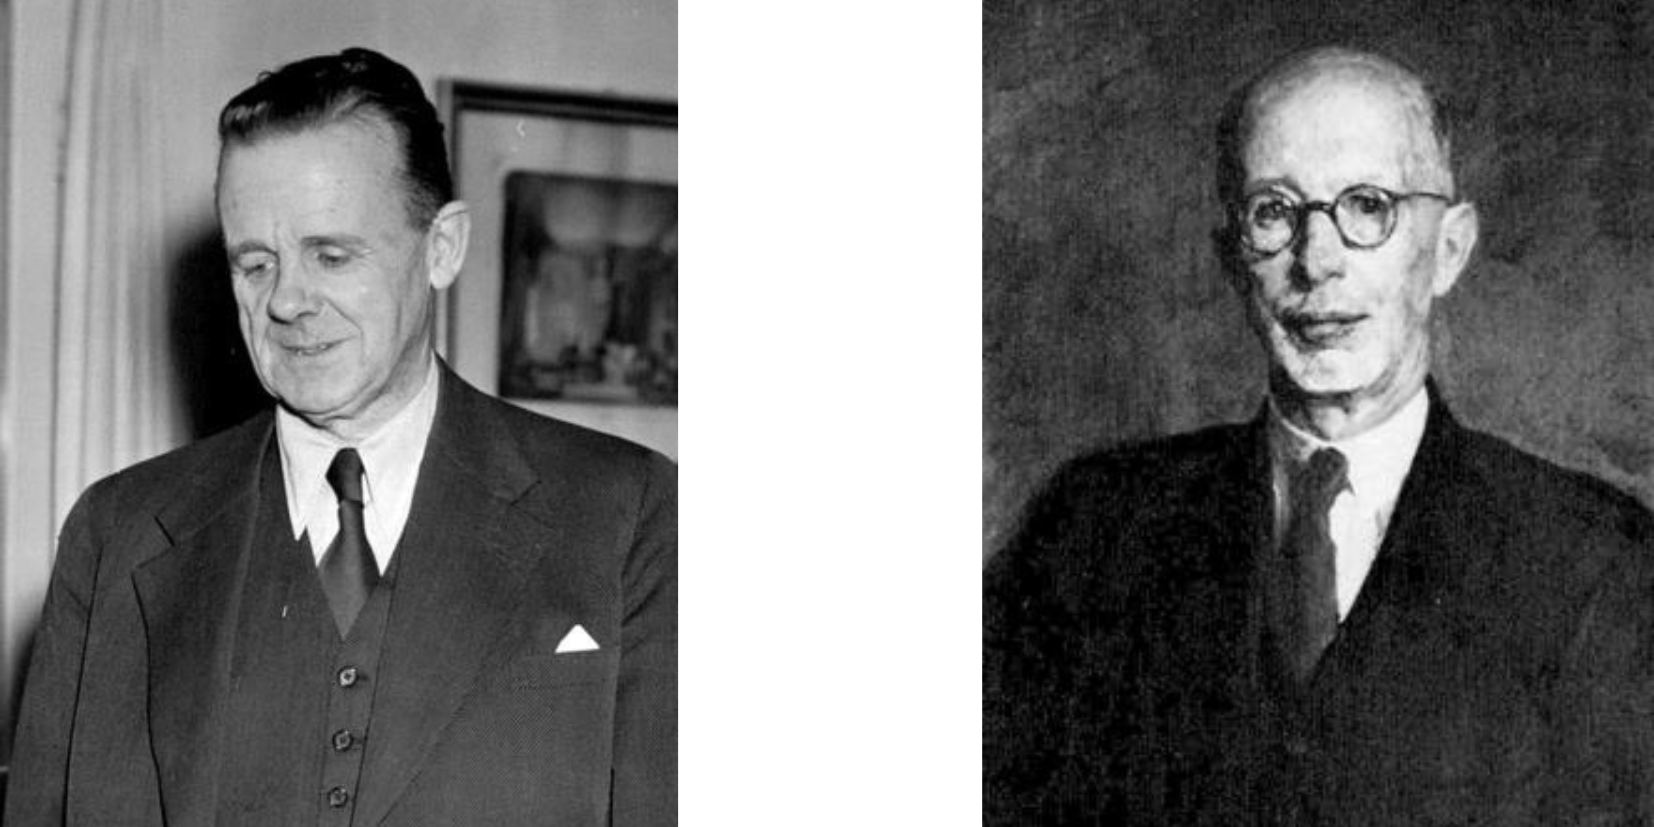
\includegraphics[width=3.125in,height=\textheight,keepaspectratio]{Diseño sin título.png}

}

\caption{Harald Cramér - Filip Lundberg}

\end{figure}%

Este modelo describe el \textbf{superávit de una aseguradora} que recibe
ingresos por primas y, a su vez, paga los montos de las reclamaciones o
siniestros que ocurren.

En términos más técnicos, el \textbf{modelo de Cramér-Lundberg} se
utiliza para estudiar la \textbf{probabilidad de ruina} de una compañía
de seguros. Aquí están algunos conceptos clave:

\begin{enumerate}
\def\labelenumi{\arabic{enumi}.}
\item
  \textbf{Proceso de Riesgo Clásico}: El capital de la compañía se
  modela como un \textbf{proceso de riesgo}, donde las primas ingresan y
  las reclamaciones salen. La probabilidad de ruina se refiere al riesgo
  de que la compañía no pueda cumplir con sus obligaciones debido a
  insuficiencia de capital.
\item
  \textbf{Distribuciones de Reclamaciones}: Se supone que las
  \textbf{distribuciones del tamaño de los reclamos} son de \textbf{cola
  ligera}, lo que significa que las reclamaciones extremadamente grandes
  son poco probables pero pueden tener un impacto significativo en la
  solvencia de la compañía.
\item
  \textbf{Fórmulas Exactas y Aproximadas}: Se han desarrollado
  \textbf{métodos} para obtener \textbf{fórmulas exactas y aproximadas}
  para la probabilidad de ruina en este modelo. Estas fórmulas permiten
  estimar la posibilidad de que la compañía quiebre debido a pérdidas
  inesperadas.
\item
  \textbf{Simulaciones y Estimaciones}: Además de las fórmulas, se
  realizan \textbf{simulaciones} de las trayectorias del proceso de
  riesgo para diferentes niveles de capital inicial. Esto proporciona
  una perspectiva más completa de las características operativas de la
  aseguradora.
\end{enumerate}

En resumen, el \textbf{modelo de Cramér-Lundberg} es una herramienta
valiosa para evaluar el riesgo financiero en el ámbito de las compañías
de seguros y comprender las posibilidades de ruina en función de las
fluctuaciones en el capital disponible.

Las siguientes fuentes presentan información detallada sobre el modelo
Cramér - Lundberg: (\autocite{asmussen2010ruin},
\autocite{dickson1998ruin})

\section{Descripción del modelo de Cramér
Lundberg}\label{descripciuxf3n-del-modelo-de-cramuxe9r-lundberg}

El modelo de Cramér Lundberg se define enseguida como un cierto tipo de
proceso estocástico(Definición~\ref{def-proc_esto}) a tiempo discreto.

Se modela el número de reclamaciones como un proceso de Poisson
\((N(t))\) con parámetro \(\lambda t\) donde \(t\geq 0\), las pérdidas
individuales \(X_i\) son variables aleatorias independientes e
idénticamente distribuidas (i. i. d.)

\begin{enumerate}
\def\labelenumi{\arabic{enumi}.}
\item
  El proceso estocástico a tiempo discreto del monto de reclamaciones se
  define como \(\{(X_k):{k \in \mathbb{N} }\}\), donde las \(X_k\) para
  \(k = 1, 2, ...,\) son variables aleatorias
  (Definición~\ref{def-variable_aleatoria}) no negativas, independientes
  e idénticamente distribuidas y tienen función de distribución común
  \(F\), media finita denotada por \(E[X_k] = \mu\) y varianza
  \(Var(X_k) = \sigma^2 \leq \infty\).
\item
  Los tiempos de reclamación ocurren en instantes aleatorios de tiempo,
  denotados por \(T_i\), tales que \[ 0 < T_1 < T_2 < \dotsb\]
\item
  El proceso de ocurrencia de las reclamaciones es el número de
  reclamaciones contingentes en el intervalo \([0,t]\), y se define como
  sigue:
\end{enumerate}

\[N(t) = \sup \{n \geq 1: T_n \leq t  \leq 0\}.\] Por convención se
usará \(\sup \ \emptyset = 0\).

\begin{enumerate}
\def\labelenumi{\arabic{enumi}.}
\setcounter{enumi}{3}
\item
  Los tiempos entre llegadas son los tiempos que transcurren entre dos
  reclamaciones sucesivas, los cuales se denotan por
  \[Y_i = T_i \ \ \ Y_k= T_k - T_{k-1}, \ \ \ k = 2,3, \dotsb,\]donde
  las variables aleatorias \(Y_k\) son i.i.d. con distribución
  exponencial y media finita \(E[Y_1] =\frac{1}{\lambda}\).
\item
  La sucesión \(\{(X_k): k \in \mathbb{N}\}\) es independiente de la
  sucesión \(\{(Y_k):k\in \mathbb{N}\}.\)
\end{enumerate}

\begin{definition}[]\protect\hypertarget{def-2}{}\label{def-2}

El proceso de agregado de siniestros \((S(t))_{t \geq 0}\) de un
portafolio se define como:
\begin{equation}\phantomsection\label{eq-1.2}{S(t):= \left\{ \begin{array}{lcc} \sum_{i=1}^{N(t)} X_i, & si & N(t) > 0, \\ \\ 
0, & si & N(t) = 0. \end{array} \right. }\end{equation} El proceso
\((S(t))_{t\geq0}\) es un proceso de suma parcial aleatoria, que se
obtiene al sustituir el índice determinado \(n\) en la suma
\(S_n = X_1 + \dotsb + X_n\) por la variable aleatoria \(N(t):\)
\[S(t) = X_1 + \dotsb+ X_{N(t)} = S_{N(t)}, \ \ t\geq0,\]que se le
conoce como proceso compuesto. Nótese que cuando
\(Var(X_k) = \sigma^2 < \infty\), el proceso del agregado de siniestros
\((S(t))t\ge0\) comparte varias propiedades asintóticas, teorema del
límite central y la ley fuerte de los grandes números.

\end{definition}

\begin{lemma}[]\protect\hypertarget{lem-1}{}\label{lem-1}

El agregado de siniestros \((S(t))\) con \(t \geq 0\) tiene función de
distribución
\begin{equation}\phantomsection\label{eq-1.3}{G_s(x) = P[S(t) \leq x] = \sum_{n=0}^{\infty} e^{-\lambda t}\frac{(\lambda t)^n}{n!}F^{n*}(x) \ \ \ t\leq 0, x \leq 0,}\end{equation}
donde \(F^{n*}(x)= P[\sum_{i=q}^{n} X_i \leq x]\) es la n-ésima
convolución de \(F\).

\end{lemma}

\begin{proof}
Sea \(G_s(x) =P[S(t) \leq x]\), por como esta definido \(S(t)\) se
tiene:

\[G_S(x) = P[S(t) \leq x] =P\left[\sum_{i=1}^{N(t)} X_i \leq x\right].\]

Aplicando el teorema de la probabilidad total se da:

\[G_s(x) =  P[S(t) \leq x] = \sum_{n=0}^{\infty} P\left[\sum_{i=1}^{N(t)} X_i \leq x | N(t) =n \right] P[N(t) = n],
\]

dado que \(S(t)|N(t) = n\) es la suma de las \(n\) variables aleatorias
i. i. d.~con distribución \(F\), por lo que la función de distribución
acumulativa de \(S(t)|N(t)=n\) es la \(n\)-ésima convolución de \(F,\)
denotada por \(F^{n*}(n)\).

Es decir
\(P\left[\sum_{i=1}^{N(t)} X_i \leq x |N(t) = n \right] = F^{n*}(x)\)
por lo tanto \(G_s(x) = \sum_{n=0}^{\infty} F^{n*} P[N(t) =n].\)

Puesto que \(P[N(t) =n]\) sigue una distribución de Poisson con
parámetro \(\lambda t\), es decir
\(P[N(t) =n] = \frac{(\lambda t)^n e^{-\lambda t}}{n!},\)

entonces

\[
G_s(x) = \sum_{n=0}^{\infty} F^{n*} \frac{(\lambda t)^n e^{-\lambda t}}{n!}.
\]
\end{proof}

\begin{lemma}[]\protect\hypertarget{lem-2}{}\label{lem-2}

Para cada \(r \geq 0\), el proceso del agregado de siniestros
\((S(t))_{t \geq 0}\) tiene función generadora de momentos
\begin{equation}\phantomsection\label{eq-1.5}{M_{S(t)}(r) = E[e^{rS(t))}] = M_{N(t)}(ln M_{x_i}(r)).}\end{equation}

\end{lemma}

\begin{proof}
Sea \(N(t)\) el proceso de Poisson con tasa \(\lambda\) que cuenta el
número de siniestros hasta el tiempo \(t\). Sea \(X_i\) el tamaño del
\(i\)-ésimo siniestro, donde los \(X_i\)'s son variables aleatorias i.
i. d.~con función generadora de momentos \(M_{X_i}(r) = E[e^{rX_i}]\) .

Condicionando sobre el número de siniestros \(N(t)\) hasta el tiempo
\(t\) se tiene:

\[S(t)|N(t) = n = \sum_{i=1}^{n} X_i. \]

Por lo tanto, la función generadora de momentos de \(S(t)\) condicionada
en \(N(t) = n\) es:

\[E[e^{rS(t)}| N(t)=n] = E\left[e^{r\sum_{i=1}^n X_i}\right].\]

Dado que los \(X_i\) son independientes, se puede escribir esto como:

\[E\left[e^{r\sum_{i=1}^n X_i}\right]= \prod_{i=1}^n E[e^{rX_i}] = (M_{X_i}(r))^n, \]

donde \(M_{X_i}(r) = E[e^{rX_i}]\) es la función generadora de momentos
de una variable aleatoria \(X_i\).

Usando la ley de probabilidad total, se puede escribir la función
generadora de momentos de \(S(t)\) como :

\[M_{S(t)}(r) = E[e^{rS(t)}] = \sum_{n=0}^{\infty} E[e^{rS(t)}|N(t) = n]P[N(t) =n]. \]
sustituyendo la expresión para \(E[e^{rS(t)}|N(t)=n]\), se tiene:

\[M_{S_(t)}(r) = \sum_{n=0}^{\infty}(M_{X_i}(r))^nP[N(t)=n]. \]

Además sabiendo que \(N(t)\) sigue una distribución de Poisson con
parámetro \(\lambda t\), es decir,

\[P[N(t) = n] = \frac{(\lambda t)^n e^{-\lambda t}}{n!} , \]

sustituyendo en la expresión anterior se da:

\[M_{S(t)}(r) = \sum_{n=0}^{\infty} \frac{(\lambda tM_{X_i}(r))^n}{n!} = e^{-\lambda t}e^{\lambda tM_{X_i}(r)}. \]

Por lo tanto

\[
M_{S(t)}(r) = e^{\lambda t(M_{X_i}(r) -1)}.
\]

Recordando que la función generadora de momentos de \(N(t)\) de un
proceso de Poisson con tasa \(\lambda\), es

\[ M_{N(t)}(r) = E[e^{rN(t)}] = e^{\lambda t(e^r - 1)}, \]

si se sustituye \(r\) por \(ln M_{X_i}(r)\), obtenemos

\[M_{N(t)}(\ln M_{X_i}(r)) = e^{\lambda t (M_{X_i}(r) - 1)}.\]

Por lo tanto

\(M_{S(t)}(r) = M_{N(t)}(\ln M_{X_i}(r));\)

lo que demuestra el lema.
\end{proof}

\begin{definition}[]\protect\hypertarget{def-3}{}\label{def-3}

El proceso de riesgo \((U(t))_{t \geq 0}\) se define como sigue:
\begin{equation}\phantomsection\label{eq-1.7}{U(t) := u + ct - S(t) \ \ \ t\geq 0, }\end{equation}
en donde \(u \geq 0\) denota el capital inicial, \(ct\) el ingreso vía
prima durante el periodo \([0,t]\) a una tasa constante \(c > 0\) y
\(S(t)\) es el agregado de siniestros en el momento \(t\).

\end{definition}

\begin{lemma}[]\protect\hypertarget{lem-3}{}\label{lem-3}

Sea \((U(t))_{t\geq0}\) un proceso de riesgo, entonces para el modelo de
renovación se tiene que:
\begin{equation}\phantomsection\label{eq-1.10}{E[U(t)] = u + ct - \mu E[N(t)],}\end{equation}
y para el modelo clásico de Crámer-Lundberg es:
\begin{equation}\phantomsection\label{eq-1.11}{E[U(t)] = u + ct - \lambda \mu t.}\end{equation}

\end{lemma}

\begin{proof}
Sea \(U(t)\) el proceso de riesgo para \(t>0\). El proceso de riesgo se
define como:

\[
U(t) = u + ct -S(t),
\]

donde:

\begin{itemize}
\item
  \(u\) es la reserva inicial de capital,
\item
  \(c\) es la tasa de ingresos premium por unidad de tiempo,
\item
  \(S(t)\) es el agregado de siniestros hasta el tiempo \(t\), es decir,
  la suma de los tamaños de siniestros ocurridos hasta ese tiempo.
\end{itemize}

Existen dos modelos para describir \(S(t)\):

\begin{enumerate}
\def\labelenumi{\arabic{enumi}.}
\item
  Modelo de renovación: Los tiempos entre siniestros tienen una
  distribución general.
\item
  Modelo clásico de Crámer-Lundberg: Los siniestros ocurren según un
  proceso de Poisson con tasa \(\lambda\).
\end{enumerate}

Se quiere demostrar las siguientes dos expresiones para \(E[U(t)]\), la
esperanza del capital en el tiempo \(t\), para ambos modelos:

\begin{enumerate}
\def\labelenumi{\arabic{enumi}.}
\item
  Para el modelo de renovación:

  \[
  E[U(t)] = u + ct - \mu E[N(t)],
  \]

  donde \(\mu = E[X_i]\) es la esperanza del tamaño de los siniestros
  \(X_i\)\hspace{0pt}, y \(N(t)\) es el número de siniestros hasta el
  tiempo \(t\).
\item
  Para el modelo clásico de Crámer-Lundberg

  \[
  E[U(t)] = u + ct - \lambda \mu t,
  \]

  donde \(\lambda\) es la tasa del proceso de Poisson para los
  siniestros y \(\mu = E[X_i]\).
\end{enumerate}

El proceso de riesgo \(U(t)\) se puede escribir como:

\[U(t) = u + ct - S(t),\]

donde \(S(t) = \sum_{i=1}^{N(t)} X_i\)\hspace{0pt} es el agregado de
siniestros hasta el tiempo \(t\), y \(N(t)\) es el número de siniestros
hasta el tiempo \(t\), mientras que los \(X_i\)\hspace{0pt}'s son los
tamaños de siniestros i. i. d.~con \(E[X_i] = \mu\).

Así se quiere encontrar:

\[
E[U(t)] = E[u + ct - S(t)].
\]

si se sabe que \(u\) y \(c\) son constantes, se tiene:

\[
E[U(t)] = u + ct - E[S(t)].
\]

Reduciéndose a calcular \(E[S(t)]\).

En el modelo de renovación, el número de siniestros \(N(t)\) hasta el
tiempo \(t\) es un proceso de renovación general. El agregado de
siniestros \(S(t)\) es la suma de \(N(t)\) siniestros, es decir,

\[
S(t) = \sum_{i=1}^{N(t)} X_i.
\]

Dado que los \(X_i\)\hspace{0pt}'s son i. i. d.~con \(E[X_i] = \mu\), la
esperanza de \(S(t)\) es:

\[
E[S(t)] = E \left[\sum_{i=1}^{N(t)} X_i \right] = E[N(t)]E[X_i] = \mu E[N(t)].
\]

Por lo tanto, la esperanza del capital en el tiempo \(t\) es:

\[
E[U(t)] = u + ct - \mu E[N(t)].
\]

En el modelo clásico de Crámer-Lundberg, los siniestros ocurren de
acuerdo con un proceso de Poisson con tasa \(\lambda\), es decir,
\(N(t) \sim Poisson(\lambda t)\) . La esperanza del número de siniestros
es:

\[
E[N(t)] = \lambda t.
\]

entonces, la esperanza del agregado de siniestros \(S(t)\) es:

\[E[S(t)] = \mu E[N(t)] = \mu \lambda t.
\]

Por lo tanto sustituyendo esto en la expresión para \(E[U(T)]\), se
tiene:

\[
E[U(t)] = u +ct - \mu \lambda t.
\]
\end{proof}

\bookmarksetup{startatroot}

\chapter{Estudio de caso: Análisis de ventas de una empresa de comida
rápida}\label{estudio-de-caso-anuxe1lisis-de-ventas-de-una-empresa-de-comida-ruxe1pida}

\section{Descripción del problema}\label{descripciuxf3n-del-problema}

Se presentan datos que son parte de las ventas de una empresa de comida
rápida. Para brindar una mejor idea del estudio caso se presentará una
extensión de lo que es una empresa de comida rápida y una franquicia.

Una empresa de comida rápida es un tipo de negocio dentro del sector
alimenticio que se especializa en la preparación y venta de alimentos y
bebidas que pueden ser servidos y consumidos rápidamente. Estas empresas
suelen ofrecer menús estandarizados y utilizan métodos de producción en
masa para asegurar la rapidez y la eficiencia en el servicio. Algunas
características típicas de una empresa de comida rápida incluyen:

\begin{enumerate}
\def\labelenumi{\arabic{enumi}.}
\item
  Rapidez en el servicio: La principal característica es la rapidez con
  la que los clientes pueden recibir sus pedidos, generalmente en pocos
  minutos.
\item
  Menú limitado y estandarizado: Los menús suelen ser simples y
  consistentes en todas las ubicaciones de la cadena, permitiendo una
  preparación rápida y eficiente.
\item
  Precios asequibles: Los precios suelen ser más bajos en comparación
  con los restaurantes tradicionales, lo que los hace accesibles a una
  amplia gama de clientes.
\item
  Métodos de preparación eficientes: Utilizan técnicas de cocción
  rápida, como freidoras y parrillas de alta eficiencia, así como la
  pre-preparación de ingredientes.
\item
  Autoservicio y comida para llevar: Muchas de estas empresas ofrecen
  opciones de autoservicio y comida para llevar, facilitando el consumo
  rápido y conveniente.
\item
  Ambiente informal: El ambiente es generalmente informal y está
  diseñado para facilitar el flujo rápido de clientes, con áreas de
  autoservicio y estaciones de recolección de pedidos.
\end{enumerate}

Ejemplos de empresas de comida rápida incluyen grandes cadenas
internacionales como McDonald's, Burger King, KFC, Subway, Carl's Jr y
Taco Bell. Estas empresas han expandido su presencia globalmente,
adaptándose a diferentes mercados y culturas mientras mantienen su
enfoque en la rapidez y eficiencia del servicio.

Muchas de estas empresas otorga parte del derecho a operar en diferentes
franquicias.

Una franquicia es un modelo de negocio en el cual una empresa (el
franquiciador) otorga a otra parte (el franquiciado) el derecho a operar
un negocio utilizando su marca, productos, servicios y modelo operativo
a cambio de una tarifa o regalías. Este modelo permite a los
franquiciadores expandir su marca y presencia en el mercado sin tener
que invertir en nuevas ubicaciones directamente. Al mismo tiempo, ofrece
a los franquiciados la oportunidad de operar un negocio con una marca
establecida y un sistema probado. Algunas características clave de una
franquicia incluyen:

\begin{enumerate}
\def\labelenumi{\arabic{enumi}.}
\item
  Marca y sistema operativo: El franquiciado utiliza la marca comercial,
  logotipos, productos y servicios del franquiciador, así como su
  sistema operativo, que puede incluir recetas, métodos de producción,
  estrategias de marketing, entre otros.
\item
  Pago de tarifas: El franquiciado paga al franquiciador una tarifa
  inicial y, en muchos casos, regalías continuas basadas en un
  porcentaje de las ventas. Estas tarifas cubren el uso de la marca y el
  soporte continuo del franquiciador.
\item
  Capacitación y soporte: El franquiciador proporciona capacitación
  inicial y soporte continuo al franquiciado, lo cual puede incluir
  formación en gestión empresarial, operaciones, marketing y servicio al
  cliente.
\item
  Estándares y control de calidad: Para mantener la consistencia y
  calidad de la marca, el franquiciador establece estándares y
  procedimientos que los franquiciados deben seguir. Esto puede incluir
  auditorias y evaluaciones periódicas.
\item
  Contrato de franquicia: La relación entre el franquiciador y el
  franquiciado está regulada por un contrato de franquicia que detalla
  los derechos y obligaciones de ambas partes, incluyendo la duración
  del acuerdo y las condiciones de renovación.
\item
  Territorio exclusivo: A menudo, el contrato otorga al franquiciado un
  territorio exclusivo en el cual puede operar, evitando la competencia
  directa con otras franquicias de la misma marca en esa área.
\end{enumerate}

La información anterior sobre el origen o desarrollo de la comida rápida
puede fundamentarse en la consulta de: \textcite{schlosser2001fast}.

Ejemplos de negocios que utilizan el modelo de franquicia incluyen
cadenas de comida rápida (como McDonald's, Carl's Jr, Subway y KFC),
hoteles (como Marriott y Hilton), servicios de limpieza, tiendas de
conveniencia y muchos otros sectores. Este modelo permite una expansión
rápida y eficiente del negocio mientras ofrece a los emprendedores la
oportunidad de operar con el respaldo de una marca establecida.

Esta empresa ofrece en sus productos dos tipos de hamburguesas, bebidas
como sodas, cervezas y cafés. En la información de las ventas incluye
registros obtenidos por una Terminal Punto de Venta (TPV), el sistema de
pago usado en establecimientos comerciales para procesar transacciones
de venta. Permite a los comerciantes aceptar el uso de tarjetas de
crédito y débito. Se tiene registro de las ventas por cada día desde el
año 2018 a noviembre del 2020, haciendo un cierre pandémico, se
registran en dos etapas, antes de pandemia los datos a partir del 25 de
julio del 2018 al 10 de abril del 2020. Los datos después de pandemia se
registraron a partir del 3 de agosto del 2020 y cerrando finalmente el
10 de noviembre del 2020, los cuales se les aplicó una homogenización
para un buen manejo de los datos y así poder presentar un mejor
análisis.

\section{Definición de estructuras de Ciencia de
Datos}\label{definiciuxf3n-de-estructuras-de-ciencia-de-datos}

\subsection{Importación de los datos originales a
R}\label{importaciuxf3n-de-los-datos-originales-a-r}

Se cargan los datos del archivo excel al lenguaje de programación
R(Sección~\ref{sec-R}) para ser leído y almacenado en un data frame
(Sección~\ref{sec-dataframe}) con la finalidad de manipular cada uno de
los elementos de la base de datos.

\begin{Shaded}
\begin{Highlighting}[]
\NormalTok{Datos }\OtherTok{\textless{}{-}} \FunctionTok{read\_excel}\NormalTok{(}\StringTok{"C:/Users/DELL/Downloads/Datos.xlsx"}\NormalTok{, }
    \AttributeTok{col\_types =} 
\FunctionTok{c}\NormalTok{(}\StringTok{"numeric"}\NormalTok{,}\StringTok{"numeric"}\NormalTok{,}\StringTok{"numeric"}\NormalTok{,}\StringTok{"numeric"}\NormalTok{,}\StringTok{"numeric"}\NormalTok{,}
                    \StringTok{"numeric"}\NormalTok{,}\StringTok{"numeric"}\NormalTok{,}\StringTok{"numeric"}\NormalTok{,}\StringTok{"numeric"}\NormalTok{,}\StringTok{"numeric"}\NormalTok{, }
                    \StringTok{"numeric"}\NormalTok{,}\StringTok{"numeric"}\NormalTok{,}\StringTok{"numeric"}\NormalTok{,}\StringTok{"numeric"}\NormalTok{,}\StringTok{"numeric"}\NormalTok{, }
                    \StringTok{"numeric"}\NormalTok{,}\StringTok{"numeric"}\NormalTok{,}\StringTok{"numeric"}\NormalTok{,}\StringTok{"numeric"}\NormalTok{,}\StringTok{"numeric"}\NormalTok{, }
                    \StringTok{"numeric"}\NormalTok{,}\StringTok{"numeric"}\NormalTok{,}\StringTok{"numeric"}\NormalTok{,}\StringTok{"numeric"}\NormalTok{,}\StringTok{"numeric"}\NormalTok{, }
                    \StringTok{"numeric"}\NormalTok{,}\StringTok{"numeric"}\NormalTok{,}\StringTok{"numeric"}\NormalTok{,}\StringTok{"numeric"}\NormalTok{,}\StringTok{"numeric"}\NormalTok{, }
                    \StringTok{"numeric"}\NormalTok{,}\StringTok{"numeric"}\NormalTok{,}\StringTok{"numeric"}\NormalTok{,}\StringTok{"numeric"}\NormalTok{,}\StringTok{"numeric"}\NormalTok{, }
                    \StringTok{"numeric"}\NormalTok{,}\StringTok{"numeric"}\NormalTok{,}\StringTok{"numeric"}\NormalTok{,}\StringTok{"numeric"}\NormalTok{,}\StringTok{"numeric"}\NormalTok{, }
                    \StringTok{"numeric"}\NormalTok{,}\StringTok{"numeric"}\NormalTok{,}\StringTok{"numeric"}\NormalTok{,}\StringTok{"numeric"}\NormalTok{,}\StringTok{"numeric"}\NormalTok{,}
                    \StringTok{"numeric"}\NormalTok{,}\StringTok{"numeric"}\NormalTok{,}\StringTok{"numeric"}\NormalTok{,}\StringTok{"numeric"}\NormalTok{,}\StringTok{"numeric"}\NormalTok{, }
                    \StringTok{"numeric"}\NormalTok{,}\StringTok{"numeric"}\NormalTok{,}\StringTok{"numeric"}\NormalTok{,}\StringTok{"numeric"}\NormalTok{,}\StringTok{"numeric"}\NormalTok{, }
                    \StringTok{"numeric"}\NormalTok{,}\StringTok{"numeric"}\NormalTok{,}\StringTok{"numeric"}\NormalTok{,}\StringTok{"numeric"}\NormalTok{,}\StringTok{"numeric"}\NormalTok{, }
                    \StringTok{"numeric"}\NormalTok{,}\StringTok{"numeric"}\NormalTok{,}\StringTok{"numeric"}\NormalTok{,}\StringTok{"numeric"}\NormalTok{,}\StringTok{"numeric"}\NormalTok{, }
                    \StringTok{"numeric"}\NormalTok{,}\StringTok{"numeric"}\NormalTok{,}\StringTok{"numeric"}\NormalTok{,}\StringTok{"numeric"}\NormalTok{,}\StringTok{"numeric"}\NormalTok{, }
                    \StringTok{"numeric"}\NormalTok{,}\StringTok{"numeric"}\NormalTok{,}\StringTok{"numeric"}\NormalTok{,}\StringTok{"numeric"}\NormalTok{,}\StringTok{"numeric"}
\NormalTok{                        ))}

\NormalTok{Datos}
\end{Highlighting}
\end{Shaded}

\begin{verbatim}
# A tibble: 2,416 x 75
    ...1  ...2  ...3  ...4  ...5  ...6 `240519` `82253.5` `247172.9` ...10 `973`
   <dbl> <dbl> <dbl> <dbl> <dbl> <dbl>    <dbl>     <dbl>      <dbl> <dbl> <dbl>
 1    NA    NA    NA    NA    NA    NA      NA        NA         NA     NA   NA 
 2    NA    NA    NA    NA    NA    NA    9382.     9441.        NA     NA 9382.
 3  2018     7    30     4 43306    NA  188038.       NA     188038.    NA  682 
 4  2018     7    30     5 43307    NA  220827        NA     220827     NA  694 
 5  2018     7    30     6 43308    NA  240519        NA     240519     NA  762 
 6  2018     7    30     7 43309    NA  229542        NA     229542     NA  704 
 7  2018     7    30     1 43310    NA  239776.       NA     239776.    NA  706 
 8  2018     7    31     2 43311    NA  172946        NA     172946     NA  602 
 9  2018     7    31     3 43312    NA  210671        NA     210671     NA  709 
10  2018     8    31     4 43313    NA  195662        NA     195662     NA  649 
# i 2,406 more rows
# i 64 more variables: `384` <dbl>, `1136` <dbl>, ...14 <dbl>,
#   `371.753114754098` <dbl>, `2428.16666666666` <dbl>, ...17 <dbl>,
#   ...18 <dbl>, `2099` <dbl>, `222` <dbl>, `2162` <dbl>, ...22 <dbl>,
#   `1384...23` <dbl>, `559` <dbl>, `1384...25` <dbl>, ...26 <dbl>,
#   `2402` <dbl>, `658` <dbl>, `2525` <dbl>, ...30 <dbl>, `1556...31` <dbl>,
#   `462` <dbl>, `1556...33` <dbl>, ...34 <dbl>, `61` <dbl>, `57` <dbl>, ...
\end{verbatim}

Como se puede apreciar, es necesario eliminar columnas, reducido a las
columnas de las ventas de los diferentes productos que oferta la empresa
con el fin de obtener las ventas totales.

\subsection{Homogenización del total de ventas por
día}\label{homogenizaciuxf3n-del-total-de-ventas-por-duxeda}

Mediante este proceso se eliminan y se corrigen valores atípicos
(Sección~\ref{sec-outlier}), valores faltantes o alguna inconsistencia
que se presentan en los datos. Esto implica la eliminación de datos
incompletos, conocidos como datos faltantes o NA. También se renombran
cabeceras de cada columna del data frame para facilitar la lectura del
archivo.

\begin{Shaded}
\begin{Highlighting}[]
\CommentTok{\#Eliminamos las columnas con datos faltantes}
\NormalTok{datos }\OtherTok{\textless{}{-}}\NormalTok{ Datos[, }\SpecialCharTok{{-}}\FunctionTok{c}\NormalTok{(}\DecValTok{6}\NormalTok{,}\DecValTok{8}\NormalTok{,}\DecValTok{10}\NormalTok{,}\DecValTok{12}\NormalTok{,}\DecValTok{14}\NormalTok{,}\DecValTok{16}\NormalTok{,}\DecValTok{18}\NormalTok{,}\DecValTok{20}\NormalTok{,}\DecValTok{22}\NormalTok{,}\DecValTok{24}\NormalTok{, }\DecValTok{26}\NormalTok{,}\DecValTok{28}\NormalTok{, }\DecValTok{30}\NormalTok{,}\DecValTok{32}\NormalTok{, }\DecValTok{34}\NormalTok{, }\DecValTok{36}\NormalTok{,}
                    \DecValTok{38}\NormalTok{,}\DecValTok{39}\NormalTok{, }\DecValTok{40}\NormalTok{,  }\DecValTok{42}\NormalTok{, }\DecValTok{44}\NormalTok{, }\DecValTok{46}\NormalTok{, }\DecValTok{48}\NormalTok{, }\DecValTok{50}\NormalTok{,}\DecValTok{51}\NormalTok{,}\DecValTok{52}\NormalTok{, }\DecValTok{53}\NormalTok{, }\DecValTok{54}\NormalTok{,}\DecValTok{55}\NormalTok{, }\DecValTok{56}\NormalTok{, }
\DecValTok{57}\NormalTok{,}\DecValTok{58}\NormalTok{,}\DecValTok{59}\NormalTok{,}\DecValTok{60}\NormalTok{,}\DecValTok{61}\NormalTok{, }\DecValTok{62}\NormalTok{, }\DecValTok{63}\NormalTok{, }\DecValTok{64}\NormalTok{, }\DecValTok{65}\NormalTok{, }\DecValTok{66}\NormalTok{, }\DecValTok{67}\NormalTok{, }\DecValTok{68}\NormalTok{, }\DecValTok{69}\NormalTok{, }\DecValTok{70}\NormalTok{, }\DecValTok{71}\NormalTok{, }\DecValTok{73}\NormalTok{,}\DecValTok{74}\NormalTok{,}\DecValTok{72}\NormalTok{, }\DecValTok{75}\NormalTok{)]}
\CommentTok{\#Cambiar las cabeceras del data frame  }
\NormalTok{datos }\OtherTok{\textless{}{-}} \FunctionTok{data.frame}\NormalTok{(datos}\SpecialCharTok{\%\textgreater{}\%} \FunctionTok{rename}\NormalTok{(Año }\OtherTok{=}\NormalTok{ ...}\DecValTok{1}\NormalTok{ ))}
\NormalTok{datos }\OtherTok{\textless{}{-}} \FunctionTok{data.frame}\NormalTok{(datos}\SpecialCharTok{\%\textgreater{}\%} \FunctionTok{rename}\NormalTok{(}\AttributeTok{Mes =}\NormalTok{ ...}\DecValTok{2}\NormalTok{, }\AttributeTok{Semana =}\NormalTok{ ...}\DecValTok{3}\NormalTok{, }\AttributeTok{Dia=}\NormalTok{ ...}\DecValTok{4}\NormalTok{, }
                  \AttributeTok{Fecha =}\NormalTok{ ...}\DecValTok{5}\NormalTok{, }\AttributeTok{Ventas=}\NormalTok{ X240519, }
                  \AttributeTok{TotalVentas =}\NormalTok{ X247172}\FloatTok{.9}\NormalTok{,}\AttributeTok{Customers =}\NormalTok{ X973,}
                  \AttributeTok{Totalcustomers =}\NormalTok{ X1136, }
                  \AttributeTok{CH\_Promedio =}\NormalTok{ X371}\FloatTok{.753114754098}\NormalTok{, }
                  \AttributeTok{TotalCH\_Promedio =}\NormalTok{ ...}\DecValTok{17}\NormalTok{, }\AttributeTok{Burgers =}\NormalTok{ X2099,}
                  \AttributeTok{TotalBurgers =}\NormalTok{ X2162, }
                  \AttributeTok{Thickurgers =}\NormalTok{ X1384...}\DecValTok{23}\NormalTok{, }
                  \AttributeTok{TotalThickburgers =}\NormalTok{ X1384...}\DecValTok{25}\NormalTok{,}
                  \AttributeTok{Total\_Burgers =}\NormalTok{ X2402, }
                  \AttributeTok{T\_Total\_Burgers=}\NormalTok{ X2525,}\AttributeTok{Bebidas =}\NormalTok{ X1556...}\DecValTok{31}\NormalTok{,}
                  \AttributeTok{Totalbebidas =}\NormalTok{ X1556...}\DecValTok{33}\NormalTok{, }\AttributeTok{Cervezas =}\NormalTok{ X61,}
                  \AttributeTok{Totalcervezas =}\NormalTok{ X83, }\AttributeTok{Cafes =}\NormalTok{ X83,}
                  \AttributeTok{Totalcafes =}\NormalTok{ X54, }\AttributeTok{Ventas\_TPV =}\NormalTok{ X158904,}
                  \AttributeTok{Total\_Ventas\_TPV =}\NormalTok{ X173412}\FloatTok{.5}\NormalTok{,}
                  \AttributeTok{HR\_Laborales =}\NormalTok{ ...}\DecValTok{47}\NormalTok{,}
                  \AttributeTok{Total\_HR\_Laborales =}\NormalTok{ ...}\DecValTok{49}\NormalTok{ ))}
\end{Highlighting}
\end{Shaded}

Por último, se realizó la separación de la base de datos antes de la
pandemia y después de la pandemia, presentando así los data
frames(Sección~\ref{sec-dataframe}) resultantes en el siguiente código y
como se ilustra posteriormente:

\begin{Shaded}
\begin{Highlighting}[]
\CommentTok{\#Análisis de los datos:}
\CommentTok{\#Filtros por días:}
\CommentTok{\#\_\_\_\_\_\_\_\_\_\_\_\_\_\_\_\_\_\_\_\_\_\_\_\_\_\_Antes de la pandemia\_\_\_\_\_\_\_\_\_\_\_\_\_\_\_\_\_\_\_\_\_\_\_\_}

\NormalTok{fil\_before1}\OtherTok{\textless{}{-}} \FunctionTok{data.frame}\NormalTok{(}\FunctionTok{subset}\NormalTok{(datos, Año }\SpecialCharTok{\textless{}=} \DecValTok{2019}\NormalTok{))}
\NormalTok{fil\_before2}\OtherTok{\textless{}{-}} \FunctionTok{data.frame}\NormalTok{(}\FunctionTok{subset}\NormalTok{(datos, Año }\SpecialCharTok{==} \DecValTok{2020} \SpecialCharTok{\&}\NormalTok{ Mes }\SpecialCharTok{\textless{}=} \DecValTok{4}\NormalTok{))}
\NormalTok{fil\_before }\OtherTok{\textless{}{-}} \FunctionTok{rbind}\NormalTok{(fil\_before1, fil\_before2)}

\CommentTok{\#\_\_\_\_\_\_\_\_\_\_\_\_\_\_\_\_\_\_\_\_\_\_\_Después de la pandemia\_\_\_\_\_\_\_\_\_\_\_\_\_\_\_\_\_\_\_\_\_\_\_\_\_}

\NormalTok{fil\_dat\_after }\OtherTok{\textless{}{-}} \FunctionTok{data.frame}\NormalTok{(}\FunctionTok{subset}\NormalTok{(datos, Año }\SpecialCharTok{==} \DecValTok{2020} \SpecialCharTok{\&}\NormalTok{ Mes}\SpecialCharTok{\textgreater{}=}\DecValTok{8}\NormalTok{))}
\end{Highlighting}
\end{Shaded}

\subsection{Data Frame Resultante: Antes de la
pandemia}\label{data-frame-resultante-antes-de-la-pandemia}

\begin{verbatim}
    Año Mes Dia   Ventas TotalVentas
3  2018   7   4 188037.5    188037.5
4  2018   7   5 220827.0    220827.0
5  2018   7   6 240519.0    240519.0
6  2018   7   7 229542.0    229542.0
7  2018   7   1 239775.6    239775.6
8  2018   7   2 172946.0    172946.0
9  2018   7   3 210671.0    210671.0
10 2018   8   4 195662.0    195662.0
11 2018   8   5 193051.0    193051.0
12 2018   8   6 206803.0    206803.0
13 2018   8   7 219399.0    219399.0
14 2018   8   1 224106.5    224106.5
15 2018   8   2 152557.0    152557.0
16 2018   8   3 148675.5    148675.5
17 2018   8   4 142344.0    142344.0
18 2018   8   5 152189.5    152189.5
19 2018   8   6 171891.0    171891.0
20 2018   8   7 194642.5    194642.5
21 2018   8   1 210023.5    210023.5
22 2018   8   2 129751.5    129751.5
23 2018   8   3 125867.5    125867.5
24 2018   8   4 133380.0    133380.0
25 2018   8   5 135070.5    135070.5
26 2018   8   6 158927.0    158927.0
27 2018   8   7 175382.0    175382.0
28 2018   8   1 187502.0    187502.0
29 2018   8   2  78116.0     78116.0
30 2018   8   3  71871.0     71871.0
31 2018   8   4  82471.5     82471.5
32 2018   8   5  98739.5     98739.5
33 2018   8   6 131185.5    131185.5
34 2018   8   7 157909.5    157909.5
35 2018   8   1 186582.0    186582.0
36 2018   8   2  68030.0     68030.0
37 2018   8   3  71887.0     71887.0
38 2018   8   4  74843.5     74843.5
39 2018   8   5  77880.5     77880.5
40 2018   8   6 128575.0    128575.0
\end{verbatim}

\subsection{Data Frame Resultante: Después de la
pandemia}\label{data-frame-resultante-despuuxe9s-de-la-pandemia}

\begin{verbatim}
     Año Mes Dia    Ventas TotalVentas
743 2020   8   2  44908.70    53887.70
744 2020   8   3  51733.00    69538.00
745 2020   8   4  57876.95    57876.95
746 2020   8   5  47554.60    57540.10
747 2020   8   6  67138.20    70025.20
748 2020   8   7  89172.70    99932.70
749 2020   8   1 113384.70   130996.70
750 2020   8   2  40974.60    47464.60
751 2020   8   3  48520.10    57037.10
752 2020   8   4  46649.15    52529.65
753 2020   8   5  40556.90    51963.40
754 2020   8   6  70159.10    81004.10
755 2020   8   7  77736.80    89482.30
756 2020   8   1 107918.30   120988.30
757 2020   8   2  48885.80    59032.80
758 2020   8   3  48311.20    57724.70
759 2020   8   4  44658.00    46319.00
760 2020   8   5  63104.30    69302.80
761 2020   8   6  67481.30    76436.30
762 2020   8   7  89795.30   102998.80
763 2020   8   1 102744.90   118060.90
764 2020   8   2  34713.50    42455.00
765 2020   8   3  40403.40    53956.40
766 2020   8   4  47028.10    56991.10
767 2020   8   5  31703.55    45095.55
768 2020   8   6  59907.40    75201.90
769 2020   8   7  89533.40    98554.40
770 2020   8   1 103271.20   115973.20
771 2020   8   2  47309.40    59826.40
\end{verbatim}

Para realizar la identificación de las diferentes distribuciones e
implementar los gráficos como los
histogramas(Sección~\ref{sec-histogramas}) y los
boxplot(Sección~\ref{sec-boxplot}), se elaboran filtros correspondientes
para las ventas por cada día antes y después de pandemia.

Los comandos para realizar los filtros son los siguientes:

\begin{Shaded}
\begin{Highlighting}[]
\CommentTok{\#filtra los datos del día Domingo antes de la pandemia}
\NormalTok{fil\_dat\_1\_before}\OtherTok{\textless{}{-}} \FunctionTok{data.frame}\NormalTok{(}\FunctionTok{subset}\NormalTok{(fil\_before, Dia }\SpecialCharTok{==} \DecValTok{1}\NormalTok{))}
\CommentTok{\#\_\_\_\_\_\_\_\_\_\_\_\_\_\_\_\_\_\_\_\_\_\_\_\_\_\_\_\_\_\_\_\_\_\_\_\_\_\_\_\_\_\_\_\_\_\_\_\_\_\_\_\_\_\_\_\_\_\_\_}
\CommentTok{\#filtra los datos del día Lunes antes de la pandemia}
\NormalTok{fil\_dat\_2\_before}\OtherTok{\textless{}{-}} \FunctionTok{data.frame}\NormalTok{(}\FunctionTok{subset}\NormalTok{(fil\_before, Dia }\SpecialCharTok{==} \DecValTok{2}\NormalTok{))}
\CommentTok{\#\_\_\_\_\_\_\_\_\_\_\_\_\_\_\_\_\_\_\_\_\_\_\_\_\_\_\_\_\_\_\_\_\_\_\_\_\_\_\_\_\_\_\_\_\_\_\_\_\_\_\_\_\_\_\_\_\_\_\_}
\CommentTok{\#filtra los datos del día martes antes de la pandemia}
\NormalTok{fil\_dat\_3\_before}\OtherTok{\textless{}{-}} \FunctionTok{data.frame}\NormalTok{(}\FunctionTok{subset}\NormalTok{(fil\_before, Dia }\SpecialCharTok{==} \DecValTok{3}\NormalTok{))}
\CommentTok{\#\_\_\_\_\_\_\_\_\_\_\_\_\_\_\_\_\_\_\_\_\_\_\_\_\_\_\_\_\_\_\_\_\_\_\_\_\_\_\_\_\_\_\_\_\_\_\_\_\_\_\_\_\_\_\_\_\_\_\_}
\CommentTok{\#filtra los datos del día miércoles antes de la pandemia}
\NormalTok{fil\_dat\_4\_before}\OtherTok{\textless{}{-}} \FunctionTok{data.frame}\NormalTok{(}\FunctionTok{subset}\NormalTok{(fil\_before, Dia }\SpecialCharTok{==} \DecValTok{4}\NormalTok{))}
\CommentTok{\#\_\_\_\_\_\_\_\_\_\_\_\_\_\_\_\_\_\_\_\_\_\_\_\_\_\_\_\_\_\_\_\_\_\_\_\_\_\_\_\_\_\_\_\_\_\_\_\_\_\_\_\_\_\_\_\_\_\_\_}
\CommentTok{\#filtra los datos del día Jueves antes de la pandemia}
\NormalTok{fil\_dat\_5\_before}\OtherTok{\textless{}{-}} \FunctionTok{data.frame}\NormalTok{(}\FunctionTok{subset}\NormalTok{(fil\_before, Dia }\SpecialCharTok{==} \DecValTok{5}\NormalTok{))}
\CommentTok{\#\_\_\_\_\_\_\_\_\_\_\_\_\_\_\_\_\_\_\_\_\_\_\_\_\_\_\_\_\_\_\_\_\_\_\_\_\_\_\_\_\_\_\_\_\_\_\_\_\_\_\_\_\_\_\_\_\_\_\_}
\CommentTok{\#filtra los datos del día Viernes antes de la pandemia}
\NormalTok{fil\_dat\_6\_before}\OtherTok{\textless{}{-}} \FunctionTok{data.frame}\NormalTok{(}\FunctionTok{subset}\NormalTok{(fil\_before, Dia }\SpecialCharTok{==} \DecValTok{6}\NormalTok{))}
\CommentTok{\#\_\_\_\_\_\_\_\_\_\_\_\_\_\_\_\_\_\_\_\_\_\_\_\_\_\_\_\_\_\_\_\_\_\_\_\_\_\_\_\_\_\_\_\_\_\_\_\_\_\_\_\_\_\_\_\_\_\_\_}
\CommentTok{\#filtra los datos del día Sábado antes de la pandemia}
\NormalTok{fil\_dat\_7\_before}\OtherTok{\textless{}{-}} \FunctionTok{data.frame}\NormalTok{(}\FunctionTok{subset}\NormalTok{(fil\_before, Dia }\SpecialCharTok{==} \DecValTok{7}\NormalTok{))}
\end{Highlighting}
\end{Shaded}

\begin{Shaded}
\begin{Highlighting}[]
\CommentTok{\#\_\_\_\_\_\_\_\_\_\_\_\_\_\_\_\_\_\_\_\_\_\_\_\_\_\_\_\_\_\_\_\_\_\_\_\_\_\_\_\_\_\_\_\_\_\_\_\_\_\_\_\_\_\_\_\_\_\_\_\_\_\_\_\_\_\_\_\_}
\NormalTok{fil\_dat\_after }\OtherTok{\textless{}{-}} \FunctionTok{data.frame}\NormalTok{(}\FunctionTok{subset}\NormalTok{(datos, Año }\SpecialCharTok{==} \DecValTok{2020} \SpecialCharTok{\&}\NormalTok{ Mes}\SpecialCharTok{\textgreater{}=}\DecValTok{8}\NormalTok{))}
\CommentTok{\#filtra los datos del día domingo despues de la pandemia}
\NormalTok{fil\_dat\_1\_after}\OtherTok{\textless{}{-}} \FunctionTok{data.frame}\NormalTok{(}\FunctionTok{subset}\NormalTok{(datos, }
\NormalTok{                                    Año }\SpecialCharTok{==} \DecValTok{2020} \SpecialCharTok{\&}\NormalTok{ Mes }\SpecialCharTok{\textgreater{}=} \DecValTok{8} \SpecialCharTok{\&}\NormalTok{ Dia}\SpecialCharTok{==}\DecValTok{1}\NormalTok{))}
\CommentTok{\#\_\_\_\_\_\_\_\_\_\_\_\_\_\_\_\_\_\_\_\_\_\_\_\_\_\_\_\_\_\_\_\_\_\_\_\_\_\_\_\_\_\_\_\_\_\_\_\_\_\_\_\_\_\_\_\_\_\_\_\_\_\_\_\_\_\_\_\_}
\CommentTok{\#filtra los datos del día lunes despues de la pandemia}
\NormalTok{fil\_dat\_2\_after}\OtherTok{\textless{}{-}} \FunctionTok{data.frame}\NormalTok{(}\FunctionTok{subset}\NormalTok{(datos,}
\NormalTok{                                    Año }\SpecialCharTok{==} \DecValTok{2020} \SpecialCharTok{\&}\NormalTok{ Mes }\SpecialCharTok{\textgreater{}=} \DecValTok{8} \SpecialCharTok{\&}\NormalTok{ Dia }\SpecialCharTok{==}\DecValTok{2}\NormalTok{))}
\CommentTok{\#\_\_\_\_\_\_\_\_\_\_\_\_\_\_\_\_\_\_\_\_\_\_\_\_\_\_\_\_\_\_\_\_\_\_\_\_\_\_\_\_\_\_\_\_\_\_\_\_\_\_\_\_\_\_\_\_\_\_\_\_\_\_\_\_\_\_\_\_}
\CommentTok{\#filtra los datos del día martes despues de la pandemia}
\NormalTok{fil\_dat\_3\_after}\OtherTok{\textless{}{-}} \FunctionTok{data.frame}\NormalTok{(}\FunctionTok{subset}\NormalTok{(datos,}
\NormalTok{                                    Año }\SpecialCharTok{==} \DecValTok{2020} \SpecialCharTok{\&}\NormalTok{ Mes }\SpecialCharTok{\textgreater{}=} \DecValTok{8} \SpecialCharTok{\&}\NormalTok{ Dia }\SpecialCharTok{==}\DecValTok{3}\NormalTok{))}
\CommentTok{\#\_\_\_\_\_\_\_\_\_\_\_\_\_\_\_\_\_\_\_\_\_\_\_\_\_\_\_\_\_\_\_\_\_\_\_\_\_\_\_\_\_\_\_\_\_\_\_\_\_\_\_\_\_\_\_\_\_\_\_\_\_\_\_\_\_\_\_\_}
\CommentTok{\#filtra los datos del día miércoles despues de la pandemia}
\NormalTok{fil\_dat\_4\_after}\OtherTok{\textless{}{-}} \FunctionTok{data.frame}\NormalTok{(}\FunctionTok{subset}\NormalTok{(datos,}
\NormalTok{                                    Año }\SpecialCharTok{==} \DecValTok{2020} \SpecialCharTok{\&}\NormalTok{ Mes }\SpecialCharTok{\textgreater{}=} \DecValTok{8} \SpecialCharTok{\&}\NormalTok{ Dia }\SpecialCharTok{==}\DecValTok{4}\NormalTok{))}
\CommentTok{\#\_\_\_\_\_\_\_\_\_\_\_\_\_\_\_\_\_\_\_\_\_\_\_\_\_\_\_\_\_\_\_\_\_\_\_\_\_\_\_\_\_\_\_\_\_\_\_\_\_\_\_\_\_\_\_\_\_\_\_\_\_\_\_\_\_\_\_\_}
\CommentTok{\#filtra los datos del día jueves despues de la pandemia}
\NormalTok{fil\_dat\_5\_after}\OtherTok{\textless{}{-}} \FunctionTok{data.frame}\NormalTok{(}\FunctionTok{subset}\NormalTok{(datos,}
\NormalTok{                                    Año }\SpecialCharTok{==} \DecValTok{2020} \SpecialCharTok{\&}\NormalTok{ Mes }\SpecialCharTok{\textgreater{}=} \DecValTok{8} \SpecialCharTok{\&}\NormalTok{ Dia }\SpecialCharTok{==}\DecValTok{5}\NormalTok{))}
\CommentTok{\#\_\_\_\_\_\_\_\_\_\_\_\_\_\_\_\_\_\_\_\_\_\_\_\_\_\_\_\_\_\_\_\_\_\_\_\_\_\_\_\_\_\_\_\_\_\_\_\_\_\_\_\_\_\_\_\_\_\_\_\_\_\_\_\_\_\_\_\_}
\CommentTok{\#filtra los datos del día viernes despues de la pandemia}
\NormalTok{fil\_dat\_6\_after}\OtherTok{\textless{}{-}} \FunctionTok{data.frame}\NormalTok{(}\FunctionTok{subset}\NormalTok{(datos,}
\NormalTok{                                    Año }\SpecialCharTok{==} \DecValTok{2020} \SpecialCharTok{\&}\NormalTok{ Mes }\SpecialCharTok{\textgreater{}=} \DecValTok{8} \SpecialCharTok{\&}\NormalTok{ Dia }\SpecialCharTok{==}\DecValTok{6}\NormalTok{))}
\CommentTok{\#\_\_\_\_\_\_\_\_\_\_\_\_\_\_\_\_\_\_\_\_\_\_\_\_\_\_\_\_\_\_\_\_\_\_\_\_\_\_\_\_\_\_\_\_\_\_\_\_\_\_\_\_\_\_\_\_\_\_\_\_\_\_\_\_\_\_\_\_}
\CommentTok{\#filtra los datos del día sábado despues de la pandemia}
\NormalTok{fil\_dat\_7\_after}\OtherTok{\textless{}{-}} \FunctionTok{data.frame}\NormalTok{(}\FunctionTok{subset}\NormalTok{(datos,}
\NormalTok{                                    Año }\SpecialCharTok{==} \DecValTok{2020} \SpecialCharTok{\&}\NormalTok{ Mes }\SpecialCharTok{\textgreater{}=} \DecValTok{8} \SpecialCharTok{\&}\NormalTok{ Dia }\SpecialCharTok{==}\DecValTok{7}\NormalTok{))}
\end{Highlighting}
\end{Shaded}

Para visualizar gráficamente el comportamiento de las ventas por día, a
continuación se construyen los histogramas por día, en los periodos
antes y después de la pandemia.

\subsection{Análisis gráfico de las ventas por
día:}\label{anuxe1lisis-gruxe1fico-de-las-ventas-por-duxeda}

Para la generación de los gráficos se emplearon los filtros anteriores
con el fin de obtener un análisis descriptivo de cada uno de ellos.

\subsubsection{Histogramas de los datos de ventas por día antes de la
pandemia}\label{histogramas-de-los-datos-de-ventas-por-duxeda-antes-de-la-pandemia}

El código que genera estos histogramas en R es el siguiente:

\begin{Shaded}
\begin{Highlighting}[]
\CommentTok{\# muestra el gráfico de todos los histogramas de ventas por día }
\CommentTok{\# antes de la pandemia}
\FunctionTok{par}\NormalTok{(}\AttributeTok{mar=}\FunctionTok{c}\NormalTok{(}\DecValTok{2}\NormalTok{,}\DecValTok{2}\NormalTok{,}\DecValTok{2}\NormalTok{,}\DecValTok{2}\NormalTok{))}
\FunctionTok{par}\NormalTok{(}\AttributeTok{mfrow =}\FunctionTok{c}\NormalTok{(}\DecValTok{3}\NormalTok{,}\DecValTok{3}\NormalTok{))}
\FunctionTok{hist}\NormalTok{(fil\_dat\_1\_before}\SpecialCharTok{$}\NormalTok{Ventas, }
     \AttributeTok{main =} \StringTok{"Ventas día Domingo"}\NormalTok{, }\AttributeTok{xlab =} \StringTok{"Ventas"}\NormalTok{)}
\FunctionTok{hist}\NormalTok{(fil\_dat\_2\_before}\SpecialCharTok{$}\NormalTok{Ventas, }
     \AttributeTok{main =} \StringTok{"Ventas día Lunes"}\NormalTok{, }\AttributeTok{xlab =} \StringTok{"Ventas"}\NormalTok{)}
\FunctionTok{hist}\NormalTok{(fil\_dat\_3\_before}\SpecialCharTok{$}\NormalTok{Ventas,}
     \AttributeTok{main =} \StringTok{"Ventas día Martes"}\NormalTok{, }\AttributeTok{xlab =} \StringTok{"Ventas"}\NormalTok{)}
\FunctionTok{hist}\NormalTok{(fil\_dat\_4\_before}\SpecialCharTok{$}\NormalTok{Ventas, }
     \AttributeTok{main =} \StringTok{"Ventas día Miércoles"}\NormalTok{, }\AttributeTok{xlab =} \StringTok{"Ventas"}\NormalTok{)}
\FunctionTok{hist}\NormalTok{(fil\_dat\_5\_before}\SpecialCharTok{$}\NormalTok{Ventas, }
     \AttributeTok{main =} \StringTok{"Ventas día Jueves"}\NormalTok{, }\AttributeTok{xlab =} \StringTok{"Ventas"}\NormalTok{)}
\FunctionTok{hist}\NormalTok{(fil\_dat\_6\_before}\SpecialCharTok{$}\NormalTok{Ventas, }
     \AttributeTok{main =} \StringTok{"Ventas día Viernes"}\NormalTok{, }\AttributeTok{xlab =} \StringTok{"Ventas"}\NormalTok{)}
\FunctionTok{hist}\NormalTok{(fil\_dat\_7\_before}\SpecialCharTok{$}\NormalTok{Ventas, }
     \AttributeTok{main =} \StringTok{"Ventas día Sábado"}\NormalTok{, }\AttributeTok{xlab =} \StringTok{"Ventas"}\NormalTok{)}
\end{Highlighting}
\end{Shaded}

\begin{figure}[H]

{\centering 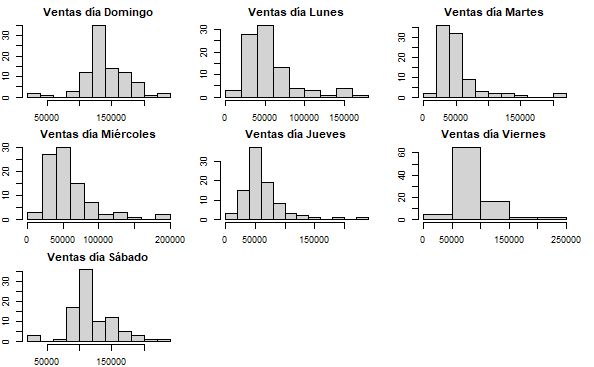
\includegraphics[width=0.8\linewidth,height=\textheight,keepaspectratio]{his_1.png}

}

\caption{Histogramas de las ventas por día antes de la pandemia.}

\end{figure}%

Para profundizar en el análisis descriptivo de las ventas periódicas se
presentan ahora los boxplot (Sección~\ref{sec-boxplot}) de las ventas
por cada día de la semana.

\subsubsection{Boxplot de datos de ventas por días antes de la
pandemia}\label{boxplot-de-datos-de-ventas-por-duxedas-antes-de-la-pandemia}

\begin{verbatim}
   Min. 1st Qu.  Median    Mean 3rd Qu.    Max. 
  30977  122963  135498  138498  158347  239776 
\end{verbatim}

\begin{verbatim}
   Min. 1st Qu.  Median    Mean 3rd Qu.    Max. 
   7430   35919   48676   57388   68030  172946 
\end{verbatim}

\begin{verbatim}
   Min. 1st Qu.  Median    Mean 3rd Qu.    Max. 
  12950   35210   44398   53367   56624  219702 
\end{verbatim}

\begin{verbatim}
   Min. 1st Qu.  Median    Mean 3rd Qu.    Max. 
  10832   35847   44213   56365   63585  195662 
\end{verbatim}

\begin{verbatim}
   Min. 1st Qu.  Median    Mean 3rd Qu.    Max. 
  13547   42368   49479   61068   70047  220827 
\end{verbatim}

\begin{verbatim}
   Min. 1st Qu.  Median    Mean 3rd Qu.    Max. 
  10331   65730   79464   86514   96522  240519 
\end{verbatim}

\begin{verbatim}
   Min. 1st Qu.  Median    Mean 3rd Qu.    Max. 
  24219  100751  110603  119332  135176  229542 
\end{verbatim}

El código que genera estos boxplot en R es el siguiente:

\begin{Shaded}
\begin{Highlighting}[]
\CommentTok{\# muestra el gráfico de todos los boxplot de ventas por día }
\CommentTok{\# antes de la pandemia }
\NormalTok{fig }\OtherTok{\textless{}{-}} \FunctionTok{plot\_ly}\NormalTok{(}\AttributeTok{y =}\NormalTok{fil\_dat\_1\_before}\SpecialCharTok{$}\NormalTok{Ventas, }\AttributeTok{name =} \StringTok{"Ventas día Domingo"}\NormalTok{, }
               \AttributeTok{boxpoints =} \StringTok{"all"}\NormalTok{,}\AttributeTok{type =} \StringTok{"box"}\NormalTok{, )}
\NormalTok{fig }\OtherTok{\textless{}{-}}\NormalTok{ fig }\SpecialCharTok{\%\textgreater{}\%} \FunctionTok{add\_trace}\NormalTok{(}\AttributeTok{y =}\NormalTok{ fil\_dat\_2\_before}\SpecialCharTok{$}\NormalTok{Ventas,  }
                         \AttributeTok{name =} \StringTok{"Ventas día Lunes"}\NormalTok{, }\AttributeTok{boxpoints =} \StringTok{"all"}\NormalTok{)}
\NormalTok{fig }\OtherTok{\textless{}{-}}\NormalTok{ fig }\SpecialCharTok{\%\textgreater{}\%} \FunctionTok{add\_trace}\NormalTok{(}\AttributeTok{y =}\NormalTok{ fil\_dat\_3\_before}\SpecialCharTok{$}\NormalTok{Ventas,  }
                         \AttributeTok{name =} \StringTok{"Ventas día Martes"}\NormalTok{, }\AttributeTok{boxpoints =} \StringTok{"all"}\NormalTok{)}
\NormalTok{fig }\OtherTok{\textless{}{-}}\NormalTok{ fig }\SpecialCharTok{\%\textgreater{}\%} \FunctionTok{add\_trace}\NormalTok{(}\AttributeTok{y =}\NormalTok{ fil\_dat\_4\_before}\SpecialCharTok{$}\NormalTok{Ventas,  }
               \AttributeTok{name =} \StringTok{"Ventas día Miércoles"}\NormalTok{, }\AttributeTok{boxpoints =} \StringTok{"all"}\NormalTok{)}
\NormalTok{fig }\OtherTok{\textless{}{-}}\NormalTok{ fig }\SpecialCharTok{\%\textgreater{}\%} \FunctionTok{add\_trace}\NormalTok{(}\AttributeTok{y =}\NormalTok{ fil\_dat\_5\_before}\SpecialCharTok{$}\NormalTok{Ventas,  }
                         \AttributeTok{name =} \StringTok{"Ventas día Jueves"}\NormalTok{, }\AttributeTok{boxpoints =} \StringTok{"all"}\NormalTok{)}
\NormalTok{fig }\OtherTok{\textless{}{-}}\NormalTok{ fig }\SpecialCharTok{\%\textgreater{}\%} \FunctionTok{add\_trace}\NormalTok{(}\AttributeTok{y =}\NormalTok{ fil\_dat\_6\_before}\SpecialCharTok{$}\NormalTok{Ventas,  }
                         \AttributeTok{name =} \StringTok{"Ventas día Viernes"}\NormalTok{, }\AttributeTok{boxpoints =} \StringTok{"all"}\NormalTok{)}
\NormalTok{fig }\OtherTok{\textless{}{-}}\NormalTok{ fig }\SpecialCharTok{\%\textgreater{}\%} \FunctionTok{add\_trace}\NormalTok{(}\AttributeTok{y =}\NormalTok{ fil\_dat\_7\_before}\SpecialCharTok{$}\NormalTok{Ventas,  }
                         \AttributeTok{name =} \StringTok{"Ventas día Sábado"}\NormalTok{, }\AttributeTok{boxpoints =} \StringTok{"all"}\NormalTok{)}

\NormalTok{fig}
\end{Highlighting}
\end{Shaded}

\begin{figure}[H]

{\centering \pandocbounded{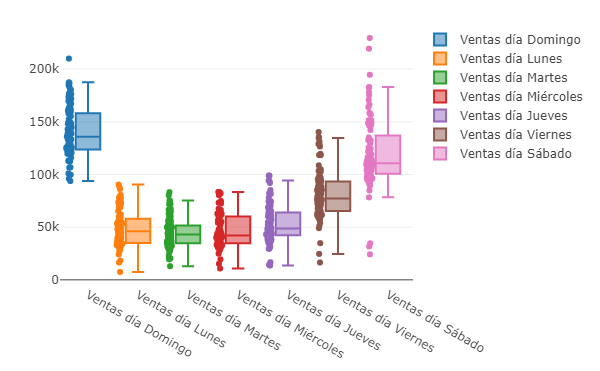
\includegraphics[keepaspectratio]{fig-box1pdf.png}}

}

\caption{Boxplot de las ventas por día antes de la pandemia.}

\end{figure}%

\subsubsection{Histogramas de los datos de ventas por día después de la
pandemia}\label{histogramas-de-los-datos-de-ventas-por-duxeda-despuuxe9s-de-la-pandemia}

El código que genera estos histogramas en R es el siguiente:

\begin{Shaded}
\begin{Highlighting}[]
\CommentTok{\# muestra el gráfico de todos los histogramas de ventas por día }
\CommentTok{\#despues de la pandemia}
\FunctionTok{par}\NormalTok{(}\AttributeTok{mar=}\FunctionTok{c}\NormalTok{(}\DecValTok{2}\NormalTok{,}\DecValTok{2}\NormalTok{,}\DecValTok{2}\NormalTok{,}\DecValTok{2}\NormalTok{))}
\FunctionTok{par}\NormalTok{(}\AttributeTok{mfrow =}\FunctionTok{c}\NormalTok{(}\DecValTok{3}\NormalTok{,}\DecValTok{3}\NormalTok{))}
\FunctionTok{hist}\NormalTok{(fil\_dat\_1\_after}\SpecialCharTok{$}\NormalTok{Ventas, }
     \AttributeTok{main =} \StringTok{"Ventas día Domingo"}\NormalTok{, }\AttributeTok{xlab =} \StringTok{"Ventas"}\NormalTok{)}
\FunctionTok{hist}\NormalTok{(fil\_dat\_2\_after}\SpecialCharTok{$}\NormalTok{Ventas, }
     \AttributeTok{main =} \StringTok{"Ventas día Lunes"}\NormalTok{, }\AttributeTok{xlab =} \StringTok{"Ventas"}\NormalTok{)}
\FunctionTok{hist}\NormalTok{(fil\_dat\_3\_after}\SpecialCharTok{$}\NormalTok{Ventas, }
     \AttributeTok{main =} \StringTok{"Ventas día Martes"}\NormalTok{, }\AttributeTok{xlab =} \StringTok{"Ventas"}\NormalTok{)}
\FunctionTok{hist}\NormalTok{(fil\_dat\_4\_after}\SpecialCharTok{$}\NormalTok{Ventas,}
     \AttributeTok{main =} \StringTok{"Ventas día Miércoles"}\NormalTok{, }\AttributeTok{xlab =} \StringTok{"Ventas"}\NormalTok{)}
\FunctionTok{hist}\NormalTok{(fil\_dat\_5\_after}\SpecialCharTok{$}\NormalTok{Ventas, }
     \AttributeTok{main =} \StringTok{"Ventas día Jueves"}\NormalTok{, }\AttributeTok{xlab =} \StringTok{"Ventas"}\NormalTok{)}
\FunctionTok{hist}\NormalTok{(fil\_dat\_6\_after}\SpecialCharTok{$}\NormalTok{Ventas, }
     \AttributeTok{main =} \StringTok{"Ventas día Viernes"}\NormalTok{, }\AttributeTok{xlab =} \StringTok{"Ventas"}\NormalTok{)}
\FunctionTok{hist}\NormalTok{(fil\_dat\_7\_after}\SpecialCharTok{$}\NormalTok{Ventas, }
     \AttributeTok{main =} \StringTok{"Ventas día Sábado"}\NormalTok{, }\AttributeTok{xlab =} \StringTok{"Ventas"}\NormalTok{)}
\end{Highlighting}
\end{Shaded}

\begin{figure}[H]

{\centering 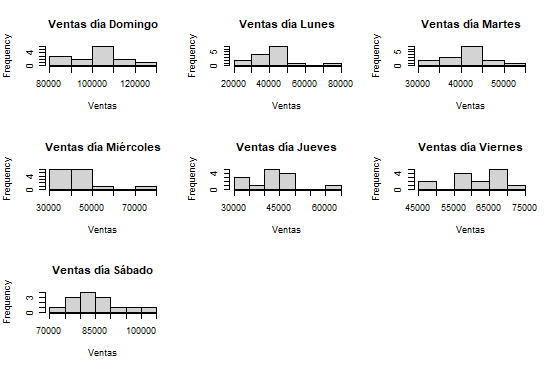
\includegraphics[width=0.8\linewidth,height=\textheight,keepaspectratio]{his_2.png}

}

\caption{Histogramas de las ventas por día después de la pandemia.}

\end{figure}%

El comportamiento periódico de las ventas se observa en los boxplot de
las ventas por cada día de la semana.

\subsubsection{Boxplot de datos de ventas por días limpios después de la
pandemia}\label{boxplot-de-datos-de-ventas-por-duxedas-limpios-despuuxe9s-de-la-pandemia}

\begin{Shaded}
\begin{Highlighting}[]
\FunctionTok{summary}\NormalTok{(fil\_dat\_1\_after}\SpecialCharTok{$}\NormalTok{Ventas)}
\end{Highlighting}
\end{Shaded}

\begin{verbatim}
   Min. 1st Qu.  Median    Mean 3rd Qu.    Max. 
  80431   95346  103691  101919  107639  122397 
\end{verbatim}

\begin{Shaded}
\begin{Highlighting}[]
\FunctionTok{summary}\NormalTok{(fil\_dat\_2\_after}\SpecialCharTok{$}\NormalTok{Ventas)}
\end{Highlighting}
\end{Shaded}

\begin{verbatim}
   Min. 1st Qu.  Median    Mean 3rd Qu.    Max. 
  27106   33867   40804   42339   47566   77299 
\end{verbatim}

\begin{Shaded}
\begin{Highlighting}[]
\FunctionTok{summary}\NormalTok{(fil\_dat\_3\_after}\SpecialCharTok{$}\NormalTok{Ventas)}
\end{Highlighting}
\end{Shaded}

\begin{verbatim}
   Min. 1st Qu.  Median    Mean 3rd Qu.    Max. 
  30514   38860   41889   41752   44732   51733 
\end{verbatim}

\begin{Shaded}
\begin{Highlighting}[]
\FunctionTok{summary}\NormalTok{(fil\_dat\_4\_after}\SpecialCharTok{$}\NormalTok{Ventas)}
\end{Highlighting}
\end{Shaded}

\begin{verbatim}
   Min. 1st Qu.  Median    Mean 3rd Qu.    Max. 
  30335   34697   43071   43243   46480   70983 
\end{verbatim}

\begin{Shaded}
\begin{Highlighting}[]
\FunctionTok{summary}\NormalTok{(fil\_dat\_5\_after}\SpecialCharTok{$}\NormalTok{Ventas)}
\end{Highlighting}
\end{Shaded}

\begin{verbatim}
   Min. 1st Qu.  Median    Mean 3rd Qu.    Max. 
  31704   39901   43144   43010   47048   63104 
\end{verbatim}

\begin{Shaded}
\begin{Highlighting}[]
\FunctionTok{summary}\NormalTok{(fil\_dat\_6\_after}\SpecialCharTok{$}\NormalTok{Ventas)}
\end{Highlighting}
\end{Shaded}

\begin{verbatim}
   Min. 1st Qu.  Median    Mean 3rd Qu.    Max. 
  45908   56956   63361   61191   66915   70159 
\end{verbatim}

\begin{Shaded}
\begin{Highlighting}[]
\FunctionTok{summary}\NormalTok{(fil\_dat\_7\_after}\SpecialCharTok{$}\NormalTok{Ventas)}
\end{Highlighting}
\end{Shaded}

\begin{verbatim}
   Min. 1st Qu.  Median    Mean 3rd Qu.    Max. 
  73606   78646   84130   85684   89730  101467 
\end{verbatim}

El código que genera estos boxplot en R es el siguiente:

\begin{Shaded}
\begin{Highlighting}[]
\CommentTok{\# muestra el gráfico de todos los boxplot de ventas por día }
\CommentTok{\# antes de la pandemia }
\NormalTok{fig }\OtherTok{\textless{}{-}} \FunctionTok{plot\_ly}\NormalTok{(}\AttributeTok{y =}\NormalTok{fil\_dat\_1\_after}\SpecialCharTok{$}\NormalTok{Ventas, }\AttributeTok{name =} \StringTok{"Ventas día Domingo"}\NormalTok{,}
               \AttributeTok{boxpoints =} \StringTok{"all"}\NormalTok{,}\AttributeTok{type =} \StringTok{"box"}\NormalTok{)}

\NormalTok{fig }\OtherTok{\textless{}{-}}\NormalTok{ fig }\SpecialCharTok{\%\textgreater{}\%} \FunctionTok{add\_trace}\NormalTok{(}\AttributeTok{y =}\NormalTok{ fil\_dat\_2\_after}\SpecialCharTok{$}\NormalTok{Ventas,  }
                         \AttributeTok{name =} \StringTok{"Ventas día Lunes"}\NormalTok{, }\AttributeTok{boxpoints =} \StringTok{"all"}\NormalTok{)}
\NormalTok{fig }\OtherTok{\textless{}{-}}\NormalTok{ fig }\SpecialCharTok{\%\textgreater{}\%} \FunctionTok{add\_trace}\NormalTok{(}\AttributeTok{y =}\NormalTok{ fil\_dat\_3\_after}\SpecialCharTok{$}\NormalTok{Ventas,  }
                         \AttributeTok{name =} \StringTok{"Ventas día Martes"}\NormalTok{, }\AttributeTok{boxpoints =} \StringTok{"all"}\NormalTok{)}
\NormalTok{fig }\OtherTok{\textless{}{-}}\NormalTok{ fig }\SpecialCharTok{\%\textgreater{}\%} \FunctionTok{add\_trace}\NormalTok{(}\AttributeTok{y =}\NormalTok{ fil\_dat\_4\_after}\SpecialCharTok{$}\NormalTok{Ventas,  }
                         \AttributeTok{name =} \StringTok{"Ventas día Miércoles"}\NormalTok{, }\AttributeTok{boxpoints =} \StringTok{"all"}\NormalTok{)}
\NormalTok{fig }\OtherTok{\textless{}{-}}\NormalTok{ fig }\SpecialCharTok{\%\textgreater{}\%} \FunctionTok{add\_trace}\NormalTok{(}\AttributeTok{y =}\NormalTok{ fil\_dat\_5\_after}\SpecialCharTok{$}\NormalTok{Ventas,  }
                         \AttributeTok{name =} \StringTok{"Ventas día Jueves"}\NormalTok{, }\AttributeTok{boxpoints =} \StringTok{"all"}\NormalTok{)}
\NormalTok{fig }\OtherTok{\textless{}{-}}\NormalTok{ fig }\SpecialCharTok{\%\textgreater{}\%} \FunctionTok{add\_trace}\NormalTok{(}\AttributeTok{y =}\NormalTok{ fil\_dat\_6\_after}\SpecialCharTok{$}\NormalTok{Ventas,  }
                         \AttributeTok{name =} \StringTok{"Ventas día Viernes"}\NormalTok{, }\AttributeTok{boxpoints=}\StringTok{"all"}\NormalTok{)}
\NormalTok{fig }\OtherTok{\textless{}{-}}\NormalTok{ fig }\SpecialCharTok{\%\textgreater{}\%} \FunctionTok{add\_trace}\NormalTok{(}\AttributeTok{y =}\NormalTok{ fil\_dat\_7\_after}\SpecialCharTok{$}\NormalTok{Ventas,  }
                         \AttributeTok{name =} \StringTok{"Ventas día Sábado"}\NormalTok{, }\AttributeTok{boxpoints =} \StringTok{"all"}\NormalTok{)}
\NormalTok{fig}
\end{Highlighting}
\end{Shaded}

\begin{figure}[H]

{\centering \pandocbounded{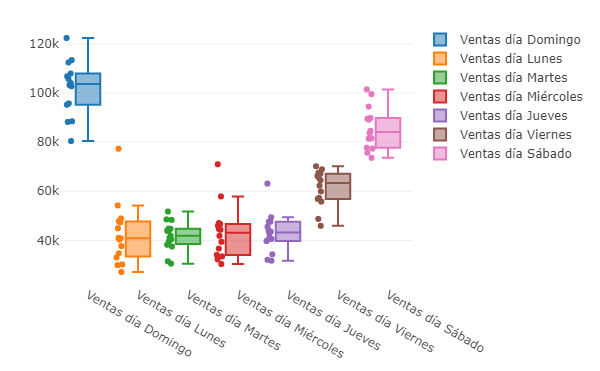
\includegraphics[keepaspectratio]{fig-box2pdf.png}}

}

\caption{Boxplot de las ventas por día después de la pandemia.}

\end{figure}%

\section{Identificación de distribuciones de probabilidad de las ventas
por
día}\label{identificaciuxf3n-de-distribuciones-de-probabilidad-de-las-ventas-por-duxeda}

Con el fin de adaptar el modelo de Cramér-Lundberg es necesario ajustar
distribuciones de probabilidad de las ventas para cada día de la semana.
Haciendo uso del test de Jarque Bera (Sección~\ref{sec-J_B}) que ayuda a
identificar cuales días siguen una distribución normal y el test de
Kolmogorov de Smirnov (Sección~\ref{sec-K_S}).

El siguiente código aplica los diferentes test de normalidad
(Sección~\ref{sec-normalidad}) para las ventas por día antes de la
pandemia:

\begin{Shaded}
\begin{Highlighting}[]
\CommentTok{\#Calcularemos los test correspondientes a los filtros}
\CommentTok{\#de ventas por día:}

\CommentTok{\#JARQUE BERA}
\FunctionTok{jarque.bera.test}\NormalTok{(fil\_dat\_1\_before}\SpecialCharTok{$}\NormalTok{Ventas)}
\end{Highlighting}
\end{Shaded}

\begin{verbatim}

    Jarque Bera Test

data:  fil_dat_1_before$Ventas
X-squared = 4.3177, df = 2, p-value = 0.1155
\end{verbatim}

\begin{Shaded}
\begin{Highlighting}[]
\CommentTok{\#El valor p no es menor que α = .05, }
\CommentTok{\#entonces hay evidencia suficiente para decir }
\CommentTok{\#por lo tanto los datos se distribuyen normalmente}
\CommentTok{\#Se ajustara una distribuciión con el comando siguiente:}

\FunctionTok{fitdistr}\NormalTok{(fil\_dat\_1\_before}\SpecialCharTok{$}\NormalTok{Ventas, }\StringTok{"normal"}\NormalTok{)}
\end{Highlighting}
\end{Shaded}

\begin{verbatim}
      mean          sd    
  139929.468    24521.524 
 (  2675.518) (  1891.877)
\end{verbatim}

\begin{Shaded}
\begin{Highlighting}[]
\CommentTok{\#JARQUE BERA}
\FunctionTok{jarque.bera.test}\NormalTok{(fil\_dat\_2\_before}\SpecialCharTok{$}\NormalTok{Ventas)}
\end{Highlighting}
\end{Shaded}

\begin{verbatim}

    Jarque Bera Test

data:  fil_dat_2_before$Ventas
X-squared = 2.7606, df = 2, p-value = 0.2515
\end{verbatim}

\begin{Shaded}
\begin{Highlighting}[]
\CommentTok{\#El valor p no es menor que α = .05, }
\CommentTok{\#entonces hay evidencia suficiente para decir }
\CommentTok{\#por lo tanto los datos se distribuyen normalmente}
\CommentTok{\#Se ajustara una distribuciión con el comando siguiente:}
\CommentTok{\#ajustamos una distribución (normal)}
\FunctionTok{fitdistr}\NormalTok{(fil\_dat\_2\_before}\SpecialCharTok{$}\NormalTok{Ventas, }\StringTok{"normal"}\NormalTok{)}
\end{Highlighting}
\end{Shaded}

\begin{verbatim}
     mean         sd    
  48125.734   17150.338 
 ( 1917.466) ( 1355.853)
\end{verbatim}

\begin{Shaded}
\begin{Highlighting}[]
\CommentTok{\#JARQUE BERA}
\FunctionTok{jarque.bera.test}\NormalTok{(fil\_dat\_3\_before}\SpecialCharTok{$}\NormalTok{Ventas)}
\end{Highlighting}
\end{Shaded}

\begin{verbatim}

    Jarque Bera Test

data:  fil_dat_3_before$Ventas
X-squared = 4.6048, df = 2, p-value = 0.1
\end{verbatim}

\begin{Shaded}
\begin{Highlighting}[]
\CommentTok{\#El valor p no es menor que α = .05, }
\CommentTok{\#entonces hay evidencia suficiente para decir }
\CommentTok{\#por lo tanto los datos se distribuyen normalmente}
\CommentTok{\#Se ajustara una distribuciión con el comando siguiente:}
\CommentTok{\#ajustamos una distribución (normal)}
\FunctionTok{fitdistr}\NormalTok{(fil\_dat\_3\_before}\SpecialCharTok{$}\NormalTok{Ventas, }\StringTok{"normal"}\NormalTok{)}
\end{Highlighting}
\end{Shaded}

\begin{verbatim}
     mean         sd    
  44509.755   14312.338 
 ( 1590.260) ( 1124.483)
\end{verbatim}

\begin{Shaded}
\begin{Highlighting}[]
\CommentTok{\#JARQUE BERA}
\FunctionTok{jarque.bera.test}\NormalTok{(fil\_dat\_4\_before}\SpecialCharTok{$}\NormalTok{Ventas)}
\end{Highlighting}
\end{Shaded}

\begin{verbatim}

    Jarque Bera Test

data:  fil_dat_4_before$Ventas
X-squared = 3.3204, df = 2, p-value = 0.1901
\end{verbatim}

\begin{Shaded}
\begin{Highlighting}[]
\CommentTok{\#El valor p no es menor que α = .05, }
\CommentTok{\#entonces hay evidencia suficiente para decir }
\CommentTok{\#por lo tanto los datos se distribuyen normalmente}
\CommentTok{\#Se ajustara una distribuciión con el comando siguiente:}
\CommentTok{\#ajustamos una distribución (normal)}
\FunctionTok{fitdistr}\NormalTok{(fil\_dat\_4\_before}\SpecialCharTok{$}\NormalTok{Ventas, }\StringTok{"normal"}\NormalTok{)}
\end{Highlighting}
\end{Shaded}

\begin{verbatim}
     mean         sd    
  46904.516   16238.151 
 ( 1815.480) ( 1283.739)
\end{verbatim}

\begin{Shaded}
\begin{Highlighting}[]
\CommentTok{\#JARQUE BERA}
\FunctionTok{jarque.bera.test}\NormalTok{(fil\_dat\_5\_before}\SpecialCharTok{$}\NormalTok{Ventas)}
\end{Highlighting}
\end{Shaded}

\begin{verbatim}

    Jarque Bera Test

data:  fil_dat_5_before$Ventas
X-squared = 4.553, df = 2, p-value = 0.1026
\end{verbatim}

\begin{Shaded}
\begin{Highlighting}[]
\CommentTok{\#El valor p no es menor que α = .05, }
\CommentTok{\#entonces hay evidencia suficiente para decir }
\CommentTok{\#por lo tanto los datos se distribuyen normalmente}
\CommentTok{\#Se ajustara una distribuciión con el comando siguiente:}
\CommentTok{\#ajustamos una distribución (normal)}
\FunctionTok{fitdistr}\NormalTok{(fil\_dat\_5\_before}\SpecialCharTok{$}\NormalTok{Ventas, }\StringTok{"normal"}\NormalTok{)}
\end{Highlighting}
\end{Shaded}

\begin{verbatim}
     mean         sd    
  52786.734   18403.175 
 ( 2032.291) ( 1437.047)
\end{verbatim}

\begin{Shaded}
\begin{Highlighting}[]
\CommentTok{\#JARQUE BERA}
\FunctionTok{jarque.bera.test}\NormalTok{(fil\_dat\_6\_before}\SpecialCharTok{$}\NormalTok{Ventas)}
\end{Highlighting}
\end{Shaded}

\begin{verbatim}

    Jarque Bera Test

data:  fil_dat_6_before$Ventas
X-squared = 2.5406, df = 2, p-value = 0.2808
\end{verbatim}

\begin{Shaded}
\begin{Highlighting}[]
\CommentTok{\#El valor p no es menor que α = .05, }
\CommentTok{\#entonces hay evidencia suficiente para decir }
\CommentTok{\#por lo tanto los datos se distribuyen normalmente}
\CommentTok{\#Se ajustara una distribuciión con el comando siguiente:}
\CommentTok{\#ajustamos una distribución (normal)}
\FunctionTok{fitdistr}\NormalTok{(fil\_dat\_6\_before}\SpecialCharTok{$}\NormalTok{Ventas, }\StringTok{"normal"}\NormalTok{)}
\end{Highlighting}
\end{Shaded}

\begin{verbatim}
     mean         sd    
  81601.876   23756.037 
 ( 2591.996) ( 1832.818)
\end{verbatim}

Para el caso del día sábado, denotado como séptimo día, no se obtuvo una
distribución normal por lo que se utilizo la paqueteria de R
\href{https://cran.r-project.org/web/packages/fitdistrplus/index.html}{fitdistrplus}
para probar el ajuste de otras distribuciones clásicas de probabilidad.
Las distribuciones probadas se presentan en el código siguiente:

\begin{Shaded}
\begin{Highlighting}[]
\FunctionTok{fitdistr}\NormalTok{(fil\_dat\_7\_before}\SpecialCharTok{$}\NormalTok{Ventas, }\StringTok{"weibull"}\NormalTok{)}
\end{Highlighting}
\end{Shaded}

\begin{verbatim}
      shape          scale    
  3.646021e+00   1.335448e+05 
 (2.784858e-01) (4.365588e+03)
\end{verbatim}

\begin{Shaded}
\begin{Highlighting}[]
\FunctionTok{fitdistr}\NormalTok{(fil\_dat\_7\_before}\SpecialCharTok{$}\NormalTok{Ventas, }\StringTok{"exponential"}\NormalTok{)}
\end{Highlighting}
\end{Shaded}

\begin{verbatim}
       rate    
  8.379989e-06 
 (8.882771e-07)
\end{verbatim}

\begin{Shaded}
\begin{Highlighting}[]
\FunctionTok{fitdistr}\NormalTok{(fil\_dat\_7\_before}\SpecialCharTok{$}\NormalTok{Ventas, }\StringTok{"lognormal"}\NormalTok{)}
\end{Highlighting}
\end{Shaded}

\begin{verbatim}
     meanlog        sdlog   
  11.64220349    0.33374967 
 ( 0.03537739) ( 0.02501560)
\end{verbatim}

De lo anterior podemos decir que el mejor ajuste se obtuvo al usar la
distribución Weibull.

\subsection{Prueba de la distribución
Weibull:}\label{prueba-de-la-distribuciuxf3n-weibull}

Una vez ajustada la distribución Weibull
(Definición~\ref{def-var_ale_weibull}), se prueban sus parámetros con la
aplicación del test de Kolmogorov de Smirnov (Sección~\ref{sec-K_S}). El
siguiente código implementa ambos procedimientos:

\begin{Shaded}
\begin{Highlighting}[]
\CommentTok{\# Calcularemos los test correspondientes a }
\CommentTok{\# los filtros de de ventas por día:}
\CommentTok{\#JARQUE BERA}
\FunctionTok{jarque.bera.test}\NormalTok{(fil\_dat\_7\_before}\SpecialCharTok{$}\NormalTok{Ventas)}
\end{Highlighting}
\end{Shaded}

\begin{verbatim}

    Jarque Bera Test

data:  fil_dat_7_before$Ventas
X-squared = 12.707, df = 2, p-value = 0.001741
\end{verbatim}

\begin{Shaded}
\begin{Highlighting}[]
\CommentTok{\#Fitting de de una distri bución weibull}
\CommentTok{\#fil\_dat\_7\_before$Ventas}
\NormalTok{fit.weibull }\OtherTok{\textless{}{-}} \FunctionTok{fitdist}\NormalTok{(fil\_dat\_7\_before}\SpecialCharTok{$}\NormalTok{Ventas, }\StringTok{"weibull"}\NormalTok{)}
\NormalTok{fit.weibull}
\end{Highlighting}
\end{Shaded}

\begin{verbatim}
Fitting of the distribution ' weibull ' by maximum likelihood 
Parameters:
          estimate   Std. Error
shape 4.782925e+00    0.3795562
scale 1.295015e+05 3205.0384538
\end{verbatim}

\begin{Shaded}
\begin{Highlighting}[]
\NormalTok{vector\_ventas7\_ordenados }\OtherTok{\textless{}{-}}\NormalTok{ fil\_dat\_7\_before}\SpecialCharTok{$}
\NormalTok{                      Ventas[}\FunctionTok{order}\NormalTok{(fil\_dat\_7\_before}\SpecialCharTok{$}\NormalTok{Ventas)]}
\NormalTok{n }\OtherTok{=} \DecValTok{83}
\NormalTok{F\_x }\OtherTok{=} \FunctionTok{numeric}\NormalTok{(n)}
\ControlFlowTok{for}\NormalTok{(i }\ControlFlowTok{in} \DecValTok{1}\SpecialCharTok{:}\NormalTok{n)\{}
\NormalTok{  F\_x[i] }\OtherTok{\textless{}{-}}\NormalTok{ (i}\SpecialCharTok{/}\NormalTok{ n)}
\NormalTok{\}}
\CommentTok{\#F\_x}
\NormalTok{f\_gorro\_x }\OtherTok{\textless{}{-}}  \FunctionTok{pweibull}\NormalTok{(vector\_ventas7\_ordenados,}
                       \AttributeTok{shape =} \FloatTok{4.784508e+00}\NormalTok{, }\AttributeTok{scale =}\FloatTok{1.295070e+05}\NormalTok{, }
                       \AttributeTok{lower.tail =} \ConstantTok{TRUE}\NormalTok{, }\AttributeTok{log.p =} \ConstantTok{FALSE}\NormalTok{)}
\NormalTok{ks }\OtherTok{\textless{}{-}} \FunctionTok{abs}\NormalTok{(F\_x }\SpecialCharTok{{-}}\NormalTok{ f\_gorro\_x)}
\end{Highlighting}
\end{Shaded}

\subsubsection{Representación gráfica al aplicar el test de Kolmogorov
de
Smirnov}\label{representaciuxf3n-gruxe1fica-al-aplicar-el-test-de-kolmogorov-de-smirnov}

\begin{verbatim}
[1] 0.1936014
\end{verbatim}

\begin{verbatim}
[1] 0.1492794
\end{verbatim}

\subsubsection{Valor máximo de la salida del test VS valor
crítico}\label{valor-muxe1ximo-de-la-salida-del-test-vs-valor-cruxedtico}

Una comparación de los resultados se observa en las siguientes gráfica:

\begin{figure}

\centering{

\pandocbounded{\includegraphics[keepaspectratio]{Estudio_caso_files/figure-pdf/fig-plot-1.pdf}}

}

\caption{\label{fig-plot-1}Valor máximo de la salida del test VS valor
crítico}

\end{figure}%

\begin{figure}

\centering{

\pandocbounded{\includegraphics[keepaspectratio]{Estudio_caso_files/figure-pdf/fig-plot-2.pdf}}

}

\caption{\label{fig-plot-2}Valor máximo de la salida del test VS valor
crítico}

\end{figure}%

\begin{figure}

\centering{

\pandocbounded{\includegraphics[keepaspectratio]{Estudio_caso_files/figure-pdf/fig-plot-3.pdf}}

}

\caption{\label{fig-plot-3}Valor máximo de la salida del test VS valor
crítico}

\end{figure}%

Para el periodo después de pandemia se repite la misma metodología.
Aplicamos el test de Jarque Bera ( Sección~\ref{sec-J_B}) a los datos
para cada día de la semana después de pandemia.

\begin{Shaded}
\begin{Highlighting}[]
\CommentTok{\#\_\_\_\_\_\_\_Después de la pandemia\_\_\_\_\_\_\_\_\_\_\_\_\_\_\_\_\_\_\_\_\_\_\_\_\_\_\_\_\_\_\_\_\_\_\_\_}
\CommentTok{\#El valor p no es menor que α = .05, }
\CommentTok{\#entonces hay evidencia suficiente para decir }
\CommentTok{\#que la muestra  proviene de una población con distribución normal.}
\CommentTok{\#JARQUE BERA}
\FunctionTok{jarque.bera.test}\NormalTok{(fil\_dat\_1\_after}\SpecialCharTok{$}\NormalTok{Ventas)}
\end{Highlighting}
\end{Shaded}

\begin{verbatim}

    Jarque Bera Test

data:  fil_dat_1_after$Ventas
X-squared = 0.24366, df = 2, p-value = 0.8853
\end{verbatim}

\begin{Shaded}
\begin{Highlighting}[]
\FunctionTok{fitdistr}\NormalTok{(fil\_dat\_1\_after}\SpecialCharTok{$}\NormalTok{Ventas, }\StringTok{"normal"}\NormalTok{)}
\end{Highlighting}
\end{Shaded}

\begin{verbatim}
      mean          sd    
  101919.050    10877.075 
 (  2907.021) (  2055.574)
\end{verbatim}

\begin{Shaded}
\begin{Highlighting}[]
\CommentTok{\#\_\_\_\_\_\_\_\_\_\_\_\_\_\_\_\_\_\_\_\_\_\_\_\_\_\_\_\_\_\_\_\_\_\_\_\_\_\_\_\_\_\_\_\_\_\_\_\_\_\_\_\_\_\_\_\_\_\_\_\_\_\_\_\_}
\CommentTok{\#Calcularemos los test correspondientes }
\CommentTok{\#a los filtros de de ventas por día:}
\CommentTok{\#El valor p no es menor que α = .05, }
\CommentTok{\#entonces hay evidencia suficiente para decir }
\CommentTok{\#que la muestra proviene de una población con distribución normal.}
\CommentTok{\#JARQUE BERA}
\FunctionTok{jarque.bera.test}\NormalTok{(fil\_dat\_2\_after}\SpecialCharTok{$}\NormalTok{Ventas)}
\end{Highlighting}
\end{Shaded}

\begin{verbatim}

    Jarque Bera Test

data:  fil_dat_2_after$Ventas
X-squared = 7.6934, df = 2, p-value = 0.02135
\end{verbatim}

\begin{Shaded}
\begin{Highlighting}[]
\FunctionTok{fitdistr}\NormalTok{(fil\_dat\_2\_after}\SpecialCharTok{$}\NormalTok{Ventas, }\StringTok{"normal"}\NormalTok{)}
\end{Highlighting}
\end{Shaded}

\begin{verbatim}
     mean         sd    
  42338.847   12048.124 
 ( 3110.812) ( 2199.676)
\end{verbatim}

\begin{Shaded}
\begin{Highlighting}[]
\CommentTok{\#\_\_\_\_\_\_\_\_\_\_\_\_\_\_\_\_\_\_\_\_\_\_\_\_\_\_\_\_\_\_\_\_\_\_\_\_\_\_\_\_\_\_\_\_\_\_\_\_\_\_\_\_\_\_\_\_\_\_\_\_\_\_\_\_}
\CommentTok{\#Calcularemos los test correspondientes }
\CommentTok{\# a los filtros de de ventas por día:}
\CommentTok{\#El valor p no es menor que α = .05, }
\CommentTok{\#entonces hay evidencia suficiente para decir }
\CommentTok{\#que la muestra proviene de una población con distribución normal.}
\CommentTok{\#JARQUE BERA}
\FunctionTok{jarque.bera.test}\NormalTok{(fil\_dat\_3\_after}\SpecialCharTok{$}\NormalTok{Ventas)}
\end{Highlighting}
\end{Shaded}

\begin{verbatim}

    Jarque Bera Test

data:  fil_dat_3_after$Ventas
X-squared = 0.39157, df = 2, p-value = 0.8222
\end{verbatim}

\begin{Shaded}
\begin{Highlighting}[]
\FunctionTok{fitdistr}\NormalTok{(fil\_dat\_3\_after}\SpecialCharTok{$}\NormalTok{Ventas, }\StringTok{"normal"}\NormalTok{)}
\end{Highlighting}
\end{Shaded}

\begin{verbatim}
     mean         sd    
  41751.747    5687.030 
 ( 1468.385) ( 1038.305)
\end{verbatim}

\begin{Shaded}
\begin{Highlighting}[]
\CommentTok{\#\_\_\_\_\_\_\_\_\_\_\_\_\_\_\_\_\_\_\_\_\_\_\_\_\_\_\_\_\_\_\_\_\_\_\_\_\_\_\_\_\_\_\_\_\_\_\_\_\_\_\_\_\_\_\_\_\_\_\_\_\_\_\_\_}
\CommentTok{\#Calcularemos los test correspondientes }
\CommentTok{\# a los filtros de de ventas por día:}
\CommentTok{\#El valor p no es menor que α = .05, }
\CommentTok{\#entonces hay evidencia suficiente para decir }
\CommentTok{\#que la muestra proviene de una población con distribución normal.}
\CommentTok{\#JARQUE BERA}
\FunctionTok{jarque.bera.test}\NormalTok{(fil\_dat\_4\_after}\SpecialCharTok{$}\NormalTok{Ventas)}
\end{Highlighting}
\end{Shaded}

\begin{verbatim}

    Jarque Bera Test

data:  fil_dat_4_after$Ventas
X-squared = 3.8727, df = 2, p-value = 0.1442
\end{verbatim}

\begin{Shaded}
\begin{Highlighting}[]
\FunctionTok{fitdistr}\NormalTok{(fil\_dat\_4\_after}\SpecialCharTok{$}\NormalTok{Ventas, }\StringTok{"normal"}\NormalTok{)}
\end{Highlighting}
\end{Shaded}

\begin{verbatim}
     mean         sd    
  43243.143   10517.841 
 ( 2811.011) ( 1987.685)
\end{verbatim}

\begin{Shaded}
\begin{Highlighting}[]
\CommentTok{\#\_\_\_\_\_\_\_\_\_\_\_\_\_\_\_\_\_\_\_\_\_\_\_\_\_\_\_\_\_\_\_\_\_\_\_\_\_\_\_\_\_\_\_\_\_\_\_\_\_\_\_\_\_\_\_\_\_\_\_\_\_\_\_\_}
\CommentTok{\#Calcularemos los test correspondientes }
\CommentTok{\# a los filtros de de ventas por día:}
\CommentTok{\#El valor p no es menor que α = .05, }
\CommentTok{\#entonces hay evidencia suficiente para decir }
\CommentTok{\#que la muestra proviene de una población con distribución normal.}
\CommentTok{\#JARQUE BERA}
\FunctionTok{jarque.bera.test}\NormalTok{(fil\_dat\_5\_after}\SpecialCharTok{$}\NormalTok{Ventas)}
\end{Highlighting}
\end{Shaded}

\begin{verbatim}

    Jarque Bera Test

data:  fil_dat_5_after$Ventas
X-squared = 2.0444, df = 2, p-value = 0.3598
\end{verbatim}

\begin{Shaded}
\begin{Highlighting}[]
\FunctionTok{fitdistr}\NormalTok{(fil\_dat\_5\_after}\SpecialCharTok{$}\NormalTok{Ventas, }\StringTok{"normal"}\NormalTok{)}
\end{Highlighting}
\end{Shaded}

\begin{verbatim}
     mean         sd    
  43010.307    7741.889 
 ( 2069.107) ( 1463.080)
\end{verbatim}

\begin{Shaded}
\begin{Highlighting}[]
\CommentTok{\#\_\_\_\_\_\_\_\_\_\_\_\_\_\_\_\_\_\_\_\_\_\_\_\_\_\_\_\_\_\_\_\_\_\_\_\_\_\_\_\_\_\_\_\_\_\_\_\_\_\_\_\_\_\_\_\_\_\_\_\_\_\_\_\_}
\CommentTok{\#Calcularemos los test correspondientes }
\CommentTok{\# a los filtros de de ventas por día:}
\CommentTok{\# El valor p no es menor que α = .05, }
\CommentTok{\#entonces hay evidencia suficiente para decir }
\CommentTok{\#que la muestra proviene de una población con distribución normal.}
\CommentTok{\#JARQUE BERA}
\FunctionTok{jarque.bera.test}\NormalTok{(fil\_dat\_6\_after}\SpecialCharTok{$}\NormalTok{Ventas)}
\end{Highlighting}
\end{Shaded}

\begin{verbatim}

    Jarque Bera Test

data:  fil_dat_6_after$Ventas
X-squared = 1.4585, df = 2, p-value = 0.4823
\end{verbatim}

\begin{Shaded}
\begin{Highlighting}[]
\FunctionTok{fitdistr}\NormalTok{(fil\_dat\_6\_after}\SpecialCharTok{$}\NormalTok{Ventas, }\StringTok{"normal"}\NormalTok{)}
\end{Highlighting}
\end{Shaded}

\begin{verbatim}
     mean         sd    
  61191.300    7202.989 
 ( 1925.080) ( 1361.237)
\end{verbatim}

\begin{Shaded}
\begin{Highlighting}[]
\CommentTok{\#\_\_\_\_\_\_\_\_\_\_\_\_\_\_\_\_\_\_\_\_\_\_\_\_\_\_\_\_\_\_\_\_\_\_\_\_\_\_\_\_\_\_\_\_\_\_\_\_\_\_\_\_\_\_\_\_\_\_\_\_\_\_\_\_}
\CommentTok{\#Calcularemos los test correspondientes }
\CommentTok{\# a los filtros de de ventas por día:}
\CommentTok{\#El valor p no es menor que α = .05, }
\CommentTok{\#entonces hay evidencia suficiente para decir }
\CommentTok{\#que la muestra proviene de una población con distribución normal.}
\FunctionTok{jarque.bera.test}\NormalTok{(fil\_dat\_7\_after}\SpecialCharTok{$}\NormalTok{Ventas)}
\end{Highlighting}
\end{Shaded}

\begin{verbatim}

    Jarque Bera Test

data:  fil_dat_7_after$Ventas
X-squared = 0.85511, df = 2, p-value = 0.6521
\end{verbatim}

\begin{Shaded}
\begin{Highlighting}[]
\CommentTok{\#Se ajustara una distribución con el comando siguiente:}
\FunctionTok{fitdistr}\NormalTok{(fil\_dat\_7\_after}\SpecialCharTok{$}\NormalTok{Ventas, }\StringTok{"normal"}\NormalTok{)}
\end{Highlighting}
\end{Shaded}

\begin{verbatim}
     mean         sd    
  85684.058    8371.359 
 ( 2237.340) ( 1582.038)
\end{verbatim}

Con las distribuciones identificadas de las ventas por día en los dos
periodos, ahora es posible simular las variables aleatorias de las
ventas de cada día de la semana y por lo tanto simular las ganancias de
toda la semana.

\section{Modelo Modificado de Cramér-Lundberg para identificar la
probabilidad de las ganancias insuficientes en una empresa de comida
rápida}\label{modelo-modificado-de-cramuxe9r-lundberg-para-identificar-la-probabilidad-de-las-ganancias-insuficientes-en-una-empresa-de-comida-ruxe1pida}

Como se vió en la sección (Capítulo~\ref{sec-modelo_C_L}) el Modelo de
Cramér-Lundberg (MCL) es una herramienta utilizada en el campo de la
gestión de riesgos y las finanzas para evaluar la probabilidad de
incumplimiento o pérdidas insuficientes en una empresa. Aunque no es
específicamente diseñado para analizar la variación de las ganancias de
una empresa, en particular una empresa de comida rápida, puede adaptarse
para evaluar la probabilidad de ganancias insuficientes en este tipo de
negocio, que puede llevar a la decisión de cierre de las actividades de
la empresa.

Para ello la ecuación general del modelo modificado que representa la
evolución de las ganancias en el tiempo hasta la semana \(t\), denotada
por \(G\) queda definida como:
\begin{equation}\phantomsection\label{eq-4.1pdf}{G(t) = u -ct + V(t), \ \ t = 1, 2, 3, ...}\end{equation}

la cual se estudiara en los dos periodo de tiempo (pre-pandemia,
pos-pandemia).

\begin{itemize}
\item
  \(V(t)\): son los ingresos de las ganancias por día para cada semana
\item
  \(c\) : Son los costos de las obligaciones financieras del
  inversionista, como préstamos, pagos por adquisición de la franquicia,
  compras de equipos inmobiliarios, pagos de empleados, etc.
\item
  \(u \geq 0\) : Es el capital inicial con el cual inicia la empresa a
  trabajar.
\end{itemize}

\subsection{Caso pre-pandemia}\label{caso-pre-pandemia}

Para la implementación del modelo modificado Cramér-Lundberg con los
datos antes de la pandemia se hizo la simulación de las variables
aleatorias mediante las distribuciones de las ventas por día tomado como
las ganancias acumuladas, y se estimó los parámetros de \(u\) y \(c\),
por lo que el modelo es determinista y se incrementa por semana.

Como se muestra en la siguiente tabla:

\begin{longtable}[]{@{}lll@{}}
\toprule\noalign{}
DÍA & MEDIA & VARIANZA \\
\midrule\noalign{}
\endhead
\bottomrule\noalign{}
\endlastfoot
Domingo & \(139929.468\) & \(601305138\) \\
Lunes & \(48125.734\) & \(294134094\) \\
Martes & \(44509.755\) & \(204843005\) \\
Miércoles & \(46904.516\) & \(263677553\) \\
Jueves & \(52786.734\) & \(338676839\) \\
Viernes & \(81601.876\) & \(564349275\) \\
Sábado & \(119112.904\) & \(620754411\) \\
\end{longtable}

\subsubsection{Modelo de Cramér-Lundberg simulado en R con datos reales
de las ventas por día de la
empresa.}\label{modelo-de-cramuxe9r-lundberg-simulado-en-r-con-datos-reales-de-las-ventas-por-duxeda-de-la-empresa.}

En la (Figura~\ref{fig-fig-trayectoriapdf}) se muestra la trayectoria
del modelo bajo los supuestos del modelo modificado. El proceso comienza
con \(t = 90\), que son las \(90\) semanas de de las ventas registradas
por día antes del cierre pandémico, con un capital inicial de
\(u= 1759629\) y una tasa de \(c= 0.29\). Los montos de las ganancias
tienen distribución Normal y Weibull.

El código que genera la trayectoria es el siguiente:

\begin{Shaded}
\begin{Highlighting}[]
\CommentTok{\# Simulación Modelo Clásico de Cramér{-}Lundberg }
\CommentTok{\# Antes de la pandemia}
\CommentTok{\# Con los datos reales de la empresa}
\FunctionTok{library}\NormalTok{(dplyr)}\CommentTok{\#librería para poder renombrar las cabeceras }
\CommentTok{\# de los dataframes}
\CommentTok{\# Parámetros}
\FunctionTok{set.seed}\NormalTok{(}\DecValTok{13}\NormalTok{) }\CommentTok{\#semilla fija}
\NormalTok{u }\OtherTok{=} \DecValTok{1759629} \CommentTok{\#surplus(capital inicial de salvamento)}
\CommentTok{\# Es un estimado a partir de la media de las ganancias por semana, }
\CommentTok{\# multiplicado por 10/3, }
\CommentTok{\# siendo una proporción para evitar la ruina}
\CommentTok{\# u (sum(medias))*(10/3)}
\NormalTok{c }\OtherTok{=}\FloatTok{0.29}\SpecialCharTok{*}\NormalTok{u }\CommentTok{\# prima de pago cada tiempo t. c=0.5*u}
\NormalTok{t\_final }\OtherTok{=} \DecValTok{90}
\CommentTok{\# S(t) = \textbackslash{}sum\_\{i=1\}\^{}\{N(t)\}X\_i}
\CommentTok{\# donde N(t)\textasciitilde{} Poisson (lambda*t)}
\CommentTok{\# X\_i \textasciitilde{} exponencial (lambda\_Xi)}
\CommentTok{\# CL = REPRESENTA EL MODELO DE CRAMER LUNDBERG}
\CommentTok{\# Simulación de trayectoria de CL\_t, cuando t \textless{} t\_final.}
\NormalTok{trayectoria\_CLt }\OtherTok{\textless{}{-}} \ControlFlowTok{function}\NormalTok{(u, c, t\_final)}
\NormalTok{\{}
\NormalTok{  tiempo }\OtherTok{\textless{}{-}} \FunctionTok{c}\NormalTok{(}\DecValTok{0}\NormalTok{)}
\NormalTok{  Cramer\_trayectoria }\OtherTok{\textless{}{-}} \FunctionTok{c}\NormalTok{(u)}
  \ControlFlowTok{while}\NormalTok{(tiempo[}\FunctionTok{length}\NormalTok{(tiempo)] }\SpecialCharTok{\textless{}}\NormalTok{ t\_final)}
\NormalTok{  \{}
\NormalTok{    tiempo\_llegada }\OtherTok{\textless{}{-}}\NormalTok{ (}\DecValTok{1}\NormalTok{)}
\NormalTok{  Y\_i }\OtherTok{\textless{}{-}}\NormalTok{  (}\FunctionTok{rnorm}\NormalTok{(}\DecValTok{1}\NormalTok{, }\AttributeTok{mean =} \FloatTok{139929.468}\NormalTok{, }\AttributeTok{sd =} \FloatTok{24521.524}\NormalTok{ )  }\SpecialCharTok{+} 
            \FunctionTok{rnorm}\NormalTok{(}\DecValTok{1}\NormalTok{, }\AttributeTok{mean =} \FloatTok{48125.734}\NormalTok{ , }\AttributeTok{sd=}\FloatTok{17150.338}\NormalTok{ )   }\SpecialCharTok{+}  
            \FunctionTok{rnorm}\NormalTok{(}\DecValTok{1}\NormalTok{, }\AttributeTok{mean =}  \FloatTok{44509.755}\NormalTok{, }\AttributeTok{sd =} \FloatTok{14312.338}\NormalTok{)  }\SpecialCharTok{+} 
            \FunctionTok{rnorm}\NormalTok{(}\DecValTok{1}\NormalTok{, }\AttributeTok{mean =}   \FloatTok{46904.516}\NormalTok{, }\AttributeTok{sd =} \FloatTok{16238.151}\NormalTok{) }\SpecialCharTok{+} 
            \FunctionTok{rnorm}\NormalTok{(}\DecValTok{1}\NormalTok{, }\AttributeTok{mean =} \FloatTok{52786.734}\NormalTok{  , }\AttributeTok{sd =} \FloatTok{18403.17}\NormalTok{)  }\SpecialCharTok{+} 
            \FunctionTok{rnorm}\NormalTok{(}\DecValTok{1}\NormalTok{, }\AttributeTok{mean =} \FloatTok{118645.9}\NormalTok{  , }\AttributeTok{sd =} \FloatTok{36530.24}\NormalTok{)   }\SpecialCharTok{+} 
    \FunctionTok{rweibull}\NormalTok{(}\DecValTok{1}\NormalTok{,  }\AttributeTok{shape =} \FloatTok{4.784508e+00}\NormalTok{, }\AttributeTok{scale =} \FloatTok{1.295070e+05}\NormalTok{ ) ) }
\NormalTok{    tiempo }\OtherTok{\textless{}{-}} \FunctionTok{c}\NormalTok{(tiempo, tiempo[}\FunctionTok{length}\NormalTok{(tiempo)] }\SpecialCharTok{+}
\NormalTok{                  tiempo\_llegada,tiempo[}\FunctionTok{length}\NormalTok{(tiempo)] }\SpecialCharTok{+}
\NormalTok{                  tiempo\_llegada ) }
\NormalTok{    Cramer\_trayectoria }\OtherTok{\textless{}{-}} \FunctionTok{c}\NormalTok{(Cramer\_trayectoria,}
\NormalTok{           Cramer\_trayectoria[}\FunctionTok{length}\NormalTok{(Cramer\_trayectoria)]}\SpecialCharTok{{-}} 
\NormalTok{                              c}\SpecialCharTok{*}\NormalTok{tiempo\_llegada,}
\NormalTok{          Cramer\_trayectoria[}\FunctionTok{length}\NormalTok{(Cramer\_trayectoria)]}\SpecialCharTok{{-}}
\NormalTok{                              c}\SpecialCharTok{*}\NormalTok{tiempo\_llegada }\SpecialCharTok{+}\NormalTok{  Y\_i )}
    \ControlFlowTok{if}\NormalTok{(Cramer\_trayectoria[}\FunctionTok{length}\NormalTok{(Cramer\_trayectoria)] }\SpecialCharTok{\textless{}} \DecValTok{0}\NormalTok{)\{}
\NormalTok{      ruina }\OtherTok{=} \DecValTok{1}
\NormalTok{    \}}
    \ControlFlowTok{else}\NormalTok{\{}
\NormalTok{      ruina }\OtherTok{=} \DecValTok{0}
\NormalTok{    \}}
\NormalTok{  \}}
\NormalTok{  df }\OtherTok{\textless{}{-}} \FunctionTok{data.frame}\NormalTok{(tiempo, Cramer\_trayectoria)}
\NormalTok{  df\_trayectoria }\OtherTok{\textless{}{-}} \FunctionTok{data.frame}\NormalTok{(df}\SpecialCharTok{\%\textgreater{}\%}\NormalTok{ rename}
\NormalTok{                               (}\AttributeTok{Tiempo =}\NormalTok{ tiempo, }
                                 \AttributeTok{Ct =}\NormalTok{ Cramer\_trayectoria))}
  \FunctionTok{return}\NormalTok{(df\_trayectoria)}
  
\NormalTok{\}}
\NormalTok{trayectoria }\OtherTok{\textless{}{-}} \FunctionTok{trayectoria\_CLt}\NormalTok{(u,c, t\_final )}

\CommentTok{\# Instalación de plotly usando github}
\CommentTok{\# devtools::install\_github("ropensci/plotly")}

\NormalTok{fig\_tr}\OtherTok{\textless{}{-}} \FunctionTok{plot\_ly}\NormalTok{(trayectoria, }\AttributeTok{x =} \SpecialCharTok{\textasciitilde{}}\NormalTok{Tiempo, }\AttributeTok{y =} \SpecialCharTok{\textasciitilde{}}\NormalTok{Ct, }
\AttributeTok{name =} \StringTok{"Ganancias: G(t)"}\NormalTok{, }\AttributeTok{type =} \StringTok{"scatter"}\NormalTok{, }\AttributeTok{mode =} \StringTok{"lines"}\NormalTok{)}
\NormalTok{fig\_tr }\OtherTok{\textless{}{-}}\NormalTok{ fig\_tr }\SpecialCharTok{\%\textgreater{}\%} \FunctionTok{add\_trace}\NormalTok{(}\AttributeTok{x =} \SpecialCharTok{\textasciitilde{}}\NormalTok{Tiempo, }\AttributeTok{y =}\NormalTok{ u,  }
\AttributeTok{name =} \StringTok{"Capital inicial: u"}\NormalTok{, }\AttributeTok{type =} \StringTok{"scatter"}\NormalTok{, }\AttributeTok{mode =} \StringTok{"lines"}\NormalTok{)}
\NormalTok{fig\_tr}
\end{Highlighting}
\end{Shaded}

\begin{figure}

\centering{

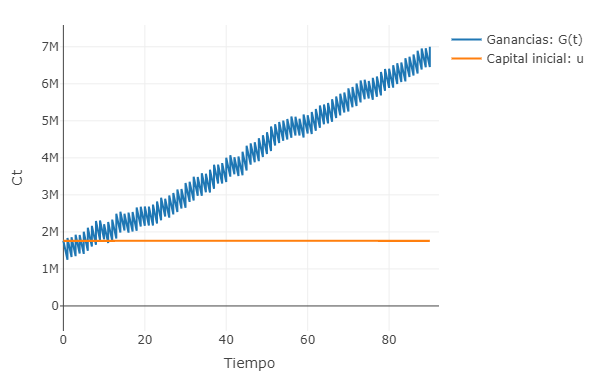
\includegraphics[width=0.8\linewidth,height=\textheight,keepaspectratio]{fig-trayectoriapdf.png}

}

\caption{\label{fig-fig-trayectoriapdf}Trayectoria del proceso de
evolución del modelo modificado de Cramér-Lundberg antes de la
pandemia.}

\end{figure}%

\subsubsection{Simulación de la probabilidad de
ruina}\label{simulaciuxf3n-de-la-probabilidad-de-ruina}

Con la simulación de la variable aleatoria \(G(t)\), es posible ahora
calcular la probabilidad de ruina, utilizando el método de Monte Carlo
(Sección~\ref{sec-Mon_Car}).

Para ello, se quiere analizar el momento en el que \(G(t)\leq u\), es
decir cuando la ganancia al final de la semana \(t\) es menor al capital
inicial. Cuando \(G(t)\leq0\), se alcanza como la ruina de la empresa,
para ambos casos se utiliza la comparación con la tasa de interés para
préstamos bancarios de \(0.8\) anual.

El código para simular la probabilidad de las ganancias finales bajas es
el siguiente:

\begin{Shaded}
\begin{Highlighting}[]
\CommentTok{\# Simulación de la probabilidad de ganancias bajas: }
\CommentTok{\# Antes de la pandemia}
\CommentTok{\# Con los datos reales de la empresa}
\FunctionTok{library}\NormalTok{(dplyr) }\CommentTok{\# librería para poder renombrar }
\CommentTok{\#las cabeceras de los dataframes}

\CommentTok{\# Parámetros}
\FunctionTok{set.seed}\NormalTok{(}\DecValTok{13}\NormalTok{) }\CommentTok{\# semilla fija}
\NormalTok{u }\OtherTok{=} \DecValTok{1759629} \CommentTok{\# surplus(capital inicial de salvamento)}
\CommentTok{\# Es un estimado a partir de la media de las ganancias por semana, }
\CommentTok{\# multiplicado por 10/3, }
\CommentTok{\# siendo una proporción para evitar la ruina}
\CommentTok{\# u (sum(medias))*(10/3)}
\NormalTok{c }\OtherTok{=} \FloatTok{0.29}\SpecialCharTok{*}\NormalTok{u }\CommentTok{\# prima de pago cada tiempo t. c = 0.5*u}
\NormalTok{lambda\_Nt }\OtherTok{=} \FloatTok{0.5}
\CommentTok{\#lambda\_Xi = 3}
\NormalTok{t\_final }\OtherTok{=} \DecValTok{48}
\NormalTok{mu }\OtherTok{=} \DecValTok{1} \CommentTok{\# tiempos entre llegadas constantes}
\NormalTok{trayectoria\_CLt }\OtherTok{\textless{}{-}} \ControlFlowTok{function}\NormalTok{(u, c, lambda\_Nt, t\_final)}
\NormalTok{\{}
\NormalTok{  tiempo }\OtherTok{\textless{}{-}} \FunctionTok{c}\NormalTok{(}\DecValTok{0}\NormalTok{)}
\NormalTok{  Cramer\_trayectoria }\OtherTok{\textless{}{-}} \FunctionTok{c}\NormalTok{(u)}
  \ControlFlowTok{while}\NormalTok{(tiempo[}\FunctionTok{length}\NormalTok{(tiempo)] }\SpecialCharTok{\textless{}}\NormalTok{ t\_final)}
\NormalTok{  \{}
\NormalTok{    tiempo\_llegada }\OtherTok{\textless{}{-}}\NormalTok{ (}\DecValTok{1}\NormalTok{) }
\CommentTok{\# Suponiendo los tiempos entrellegadas constantes \textbackslash{}mu = 1}
\NormalTok{    Y\_i }\OtherTok{\textless{}{-}}\NormalTok{  (}\FunctionTok{rnorm}\NormalTok{(}\DecValTok{1}\NormalTok{, }\AttributeTok{mean =} \FloatTok{139929.468}\NormalTok{, }\AttributeTok{sd =} \FloatTok{24521.524}\NormalTok{ ) }\SpecialCharTok{+} 
             \FunctionTok{rnorm}\NormalTok{(}\DecValTok{1}\NormalTok{, }\AttributeTok{mean =} \FloatTok{48125.734}\NormalTok{ , }\AttributeTok{sd=}\FloatTok{17150.338}\NormalTok{ ) }\SpecialCharTok{+}  
             \FunctionTok{rnorm}\NormalTok{(}\DecValTok{1}\NormalTok{, }\AttributeTok{mean =}  \FloatTok{44509.755}\NormalTok{, }\AttributeTok{sd =} \FloatTok{14312.338}\NormalTok{ ) }\SpecialCharTok{+} 
             \FunctionTok{rnorm}\NormalTok{(}\DecValTok{1}\NormalTok{, }\AttributeTok{mean =}   \FloatTok{46904.516}\NormalTok{, }\AttributeTok{sd =} \FloatTok{16238.151}\NormalTok{ ) }\SpecialCharTok{+} 
             \FunctionTok{rnorm}\NormalTok{(}\DecValTok{1}\NormalTok{, }\AttributeTok{mean =} \FloatTok{52786.734}\NormalTok{  , }\AttributeTok{sd =} \FloatTok{18403.17}\NormalTok{ ) }\SpecialCharTok{+} 
             \FunctionTok{rnorm}\NormalTok{(}\DecValTok{1}\NormalTok{, }\AttributeTok{mean =} \FloatTok{118645.9}\NormalTok{  , }\AttributeTok{sd =} \FloatTok{36530.24}\NormalTok{) }\SpecialCharTok{+}
             \FunctionTok{rweibull}\NormalTok{(}\DecValTok{1}\NormalTok{,  }\AttributeTok{shape =} \FloatTok{4.784508e+00}\NormalTok{, }\AttributeTok{scale =} \FloatTok{1.295070e+05}\NormalTok{)) }
\NormalTok{    tiempo }\OtherTok{\textless{}{-}} \FunctionTok{c}\NormalTok{(tiempo, tiempo[}\FunctionTok{length}\NormalTok{(tiempo)] }\SpecialCharTok{+}
\NormalTok{                  tiempo\_llegada,tiempo[}\FunctionTok{length}\NormalTok{(tiempo)] }\SpecialCharTok{+} 
\NormalTok{                  tiempo\_llegada ) }
\NormalTok{    Cramer\_trayectoria }\OtherTok{\textless{}{-}}\FunctionTok{c}\NormalTok{(Cramer\_trayectoria,}
\NormalTok{                Cramer\_trayectoria[}\FunctionTok{length}\NormalTok{(Cramer\_trayectoria)]}\SpecialCharTok{{-}}
\NormalTok{                  c}\SpecialCharTok{*}\NormalTok{tiempo\_llegada,}
\NormalTok{                Cramer\_trayectoria[}\FunctionTok{length}\NormalTok{(Cramer\_trayectoria)]}\SpecialCharTok{{-}}
\NormalTok{                  c}\SpecialCharTok{*}\NormalTok{tiempo\_llegada }\SpecialCharTok{+}\NormalTok{  Y\_i )}
    \ControlFlowTok{if}\NormalTok{(Cramer\_trayectoria[}\FunctionTok{length}\NormalTok{(Cramer\_trayectoria)] }\SpecialCharTok{\textless{}} \DecValTok{0}\NormalTok{)\{}
\NormalTok{      ruina }\OtherTok{=} \DecValTok{1}
\NormalTok{    \}}
    \ControlFlowTok{else}\NormalTok{\{}
\NormalTok{      ruina }\OtherTok{=} \DecValTok{0}
\NormalTok{    \}}
\NormalTok{  \}}
\CommentTok{\# 1.08*u es la ganancia inferior a la de un tasa de }
\CommentTok{\# un título financiero }
\CommentTok{\# para el año 2018}
  \ControlFlowTok{if}\NormalTok{(Cramer\_trayectoria[}\FunctionTok{length}\NormalTok{(Cramer\_trayectoria)] }\SpecialCharTok{\textless{}} \FloatTok{1.08}\SpecialCharTok{*}\NormalTok{u) \{}
\NormalTok{    ganancia\_no\_deseada }\OtherTok{=} \DecValTok{1}
    
\NormalTok{  \} }
  \ControlFlowTok{else}\NormalTok{\{}
\NormalTok{    ganancia\_no\_deseada }\OtherTok{=} \DecValTok{0}
\NormalTok{  \}}
\NormalTok{  df }\OtherTok{\textless{}{-}} \FunctionTok{data.frame}\NormalTok{(tiempo, Cramer\_trayectoria)}
\NormalTok{  df\_trayectoria }\OtherTok{\textless{}{-}} \FunctionTok{data.frame}\NormalTok{(df}\SpecialCharTok{\%\textgreater{}\%}\NormalTok{rename}
\NormalTok{                               (}\AttributeTok{Tiempo =}\NormalTok{ tiempo, }
                                \AttributeTok{Ct =}\NormalTok{ Cramer\_trayectoria))}
\NormalTok{  salida }\OtherTok{\textless{}{-}} \FunctionTok{c}\NormalTok{(ruina, ganancia\_no\_deseada)}
  \FunctionTok{return}\NormalTok{(salida)}
  
\NormalTok{\}}
\NormalTok{trayectoria }\OtherTok{\textless{}{-}} \FunctionTok{trayectoria\_CLt}\NormalTok{(u,c,lambda\_Nt, t\_final )}
\CommentTok{\# Método de monte carlo para estimar }
\CommentTok{\# la probabilidad de las ganancias bajas}
\NormalTok{n\_replicaciones }\OtherTok{=} \DecValTok{100}
\NormalTok{r\_baja\_ganancia }\OtherTok{\textless{}{-}} \FunctionTok{replicate}\NormalTok{(n\_replicaciones,}
\FunctionTok{trayectoria\_CLt}\NormalTok{(u, c, lambda\_Nt, t\_final)}
\NormalTok{[}\DecValTok{2}\NormalTok{])}
\CommentTok{\#r\_baja\_ganancia }
\NormalTok{prob\_baja\_ganancia }\OtherTok{\textless{}{-}} \FunctionTok{sum}\NormalTok{(r\_baja\_ganancia }\SpecialCharTok{\textgreater{}}\DecValTok{0}\NormalTok{)}\SpecialCharTok{/}\NormalTok{n\_replicaciones}
\end{Highlighting}
\end{Shaded}

Es claro que la evolución de \(G(t)\) antes de la pandemia genera una
probabilidad cero de las ganancias bajas.

\begin{verbatim}
[1] 0
\end{verbatim}

El código para calcular la probabilidad de ruina es el siguiente:

\begin{Shaded}
\begin{Highlighting}[]
\CommentTok{\# Simulación de la probabilidad de ruina: Antes de la pandemia}
\CommentTok{\# Con los datos reales de la empresa}
\FunctionTok{library}\NormalTok{(dplyr) }\CommentTok{\# librería para poder renombrar }
\CommentTok{\# las cabeceras de los dataframes}

\CommentTok{\# Parámetros}
\FunctionTok{set.seed}\NormalTok{(}\DecValTok{13}\NormalTok{) }\CommentTok{\# semilla fija}
\NormalTok{u }\OtherTok{=} \DecValTok{1759629} \CommentTok{\#surplus(capital inicial de salvamento)}
\CommentTok{\#Es un estimado a partir de la media de las ganancias por semana, }
\CommentTok{\#multiplicado por 10/3, }
\CommentTok{\#siendo una proporción para evitar la ruina}
\CommentTok{\# u (sum(medias))*(10/3)}
\NormalTok{c }\OtherTok{=} \FloatTok{0.29}\SpecialCharTok{*}\NormalTok{u }\CommentTok{\#prima de pago cada tiempo t. c=0.5*u}
\NormalTok{lambda\_Nt }\OtherTok{=} \FloatTok{0.5}
\CommentTok{\#lambda\_Xi = 3}
\NormalTok{t\_final }\OtherTok{=} \DecValTok{48}
\NormalTok{mu }\OtherTok{=} \DecValTok{1} \CommentTok{\#tiempos entre llegadas constantes}
\NormalTok{trayectoria\_CLt }\OtherTok{\textless{}{-}} \ControlFlowTok{function}\NormalTok{(u, c, lambda\_Nt, t\_final)}
\NormalTok{\{}
\NormalTok{  tiempo }\OtherTok{\textless{}{-}} \FunctionTok{c}\NormalTok{(}\DecValTok{0}\NormalTok{)}
\NormalTok{  Cramer\_trayectoria }\OtherTok{\textless{}{-}} \FunctionTok{c}\NormalTok{(u)}
  \ControlFlowTok{while}\NormalTok{(tiempo[}\FunctionTok{length}\NormalTok{(tiempo)] }\SpecialCharTok{\textless{}}\NormalTok{ t\_final)}
\NormalTok{  \{}
\NormalTok{    tiempo\_llegada }\OtherTok{\textless{}{-}}\NormalTok{ (}\DecValTok{1}\NormalTok{) }
\CommentTok{\#Suponiendo los tiempos entrellegadas constantes \textbackslash{}mu = 1}
\NormalTok{    Y\_i }\OtherTok{\textless{}{-}}\NormalTok{  (}\FunctionTok{rnorm}\NormalTok{(}\DecValTok{1}\NormalTok{, }\AttributeTok{mean =} \FloatTok{139929.468}\NormalTok{, }\AttributeTok{sd =} \FloatTok{24521.524}\NormalTok{ ) }\SpecialCharTok{+}
             \FunctionTok{rnorm}\NormalTok{(}\DecValTok{1}\NormalTok{, }\AttributeTok{mean =} \FloatTok{48125.734}\NormalTok{ , }\AttributeTok{sd=}\FloatTok{17150.338}\NormalTok{ )   }\SpecialCharTok{+}  
             \FunctionTok{rnorm}\NormalTok{(}\DecValTok{1}\NormalTok{, }\AttributeTok{mean =}  \FloatTok{44509.755}\NormalTok{, }\AttributeTok{sd =} \FloatTok{14312.338}\NormalTok{ ) }\SpecialCharTok{+} 
             \FunctionTok{rnorm}\NormalTok{(}\DecValTok{1}\NormalTok{, }\AttributeTok{mean =}   \FloatTok{46904.516}\NormalTok{, }\AttributeTok{sd =} \FloatTok{16238.151}\NormalTok{) }\SpecialCharTok{+} 
             \FunctionTok{rnorm}\NormalTok{(}\DecValTok{1}\NormalTok{, }\AttributeTok{mean =} \FloatTok{52786.734}\NormalTok{  , }\AttributeTok{sd =} \FloatTok{18403.17}\NormalTok{ ) }\SpecialCharTok{+}
             \FunctionTok{rnorm}\NormalTok{(}\DecValTok{1}\NormalTok{, }\AttributeTok{mean =} \FloatTok{118645.9}\NormalTok{  , }\AttributeTok{sd =} \FloatTok{36530.24}\NormalTok{)   }\SpecialCharTok{+} 
             \FunctionTok{rweibull}\NormalTok{(}\DecValTok{1}\NormalTok{,  }\AttributeTok{shape =} \FloatTok{4.784508e+00}\NormalTok{, }\AttributeTok{scale =} \FloatTok{1.295070e+05}\NormalTok{)) }
\NormalTok{    tiempo }\OtherTok{\textless{}{-}} \FunctionTok{c}\NormalTok{(tiempo, tiempo[}\FunctionTok{length}\NormalTok{(tiempo)] }\SpecialCharTok{+}
\NormalTok{                  tiempo\_llegada,tiempo[}\FunctionTok{length}\NormalTok{(tiempo)] }\SpecialCharTok{+} 
\NormalTok{                  tiempo\_llegada ) }
\NormalTok{    Cramer\_trayectoria }\OtherTok{\textless{}{-}}\FunctionTok{c}\NormalTok{(Cramer\_trayectoria,}
\NormalTok{                Cramer\_trayectoria[}\FunctionTok{length}\NormalTok{(Cramer\_trayectoria)]}\SpecialCharTok{{-}}
\NormalTok{                             c}\SpecialCharTok{*}\NormalTok{tiempo\_llegada,}
\NormalTok{                Cramer\_trayectoria[}\FunctionTok{length}\NormalTok{(Cramer\_trayectoria)]}\SpecialCharTok{{-}}
\NormalTok{                             c}\SpecialCharTok{*}\NormalTok{tiempo\_llegada }\SpecialCharTok{+}\NormalTok{  Y\_i )}
    \ControlFlowTok{if}\NormalTok{(Cramer\_trayectoria[}\FunctionTok{length}\NormalTok{(Cramer\_trayectoria)] }\SpecialCharTok{\textless{}} \DecValTok{0}\NormalTok{)\{}
\NormalTok{      ruina }\OtherTok{=} \DecValTok{1}
\NormalTok{    \}}
    \ControlFlowTok{else}\NormalTok{\{}
\NormalTok{      ruina }\OtherTok{=} \DecValTok{0}
\NormalTok{    \}}
\NormalTok{  \}}
\CommentTok{\# 1.08*u es la ganancia inferior a la de un tasa de}
\CommentTok{\# un título financiero para el año 2018}
  \ControlFlowTok{if}\NormalTok{(Cramer\_trayectoria[}\FunctionTok{length}\NormalTok{(Cramer\_trayectoria)] }\SpecialCharTok{\textless{}} \FloatTok{1.08}\SpecialCharTok{*}\NormalTok{u) \{}
\NormalTok{    ganancia\_no\_deseada }\OtherTok{=} \DecValTok{1}
    
\NormalTok{  \} }
  \ControlFlowTok{else}\NormalTok{\{}
\NormalTok{    ganancia\_no\_deseada }\OtherTok{=} \DecValTok{0}
\NormalTok{  \}}
\NormalTok{  df }\OtherTok{\textless{}{-}} \FunctionTok{data.frame}\NormalTok{(tiempo, Cramer\_trayectoria)}
\NormalTok{  df\_trayectoria }\OtherTok{\textless{}{-}} \FunctionTok{data.frame}\NormalTok{(df}\SpecialCharTok{\%\textgreater{}\%}\NormalTok{ rename}
\NormalTok{                               (}\AttributeTok{Tiempo =}\NormalTok{ tiempo, }
                                 \AttributeTok{Ct =}\NormalTok{ Cramer\_trayectoria))}
\NormalTok{  salida }\OtherTok{\textless{}{-}} \FunctionTok{c}\NormalTok{(ruina, ganancia\_no\_deseada)}
  \FunctionTok{return}\NormalTok{(salida)}
  
\NormalTok{\}}
\NormalTok{trayectoria }\OtherTok{\textless{}{-}} \FunctionTok{trayectoria\_CLt}\NormalTok{(u,c,lambda\_Nt, t\_final )}
\CommentTok{\#Método de monte carlo para estimar la probabilidad de ruina}
\NormalTok{n\_replicaciones }\OtherTok{=} \DecValTok{100}
\NormalTok{r\_ruina }\OtherTok{\textless{}{-}} \FunctionTok{replicate}\NormalTok{(n\_replicaciones, }
            \FunctionTok{trayectoria\_CLt}\NormalTok{(u, c, lambda\_Nt, t\_final)[}\DecValTok{1}\NormalTok{])}
\CommentTok{\#r\_ruina}
\NormalTok{prob\_ruin }\OtherTok{\textless{}{-}} \FunctionTok{sum}\NormalTok{(r\_ruina}\SpecialCharTok{\textgreater{}}\DecValTok{0}\NormalTok{)}\SpecialCharTok{/}\NormalTok{n\_replicaciones}
\end{Highlighting}
\end{Shaded}

En efecto, la evolución de \(G(t)\) antes de la pandemia genera una
probabilidad ruina cero.

\begin{verbatim}
[1] 0
\end{verbatim}

\subsubsection{Análisis de
sensibilidad}\label{anuxe1lisis-de-sensibilidad}

Se analiza ahora los cambios del resultado del modelo cuando se
modifican sus entradas o parámetros, por lo cual se realiza un análisis
de sensibilidad de algunos parámetros.

Para ello, del modelo modificado de Cramér-Lundberg, se toman los
parámetros \(u\) y \(c\) del modelo modificado y se establecen los
rangos o valores posibles para cada uno de los ciertos parámetros;
también se toman las medianas de las ganancias en la semana final de
\(100\) simulaciones de las trayectorias del modelo. Los rangos se
determinan hasta que el modelo presente un comportamiento diferente.

Se presenta el código para generar el análisis de sensibilidad con los
datos de las ventas de \(90\) semanas.

\begin{Shaded}
\begin{Highlighting}[]
\CommentTok{\#Simulación Modelo Clásico de Cramer{-}Lundberg: }
\CommentTok{\#Antes de la pandemia Con los datos reales de la empresa}

\FunctionTok{library}\NormalTok{(dplyr) }\CommentTok{\# librería para poder renombrar }
\CommentTok{\#las cabeceras de los dataframes}
\CommentTok{\#Parámetros}
\FunctionTok{set.seed}\NormalTok{(}\DecValTok{13}\NormalTok{) }\CommentTok{\#semilla fija}
\NormalTok{u }\OtherTok{=} \DecValTok{1759629} \CommentTok{\#surplus(capital inicial de salvamento)}
\CommentTok{\#Es un estimado a partir de la media de las ganancias por semana, }
\CommentTok{\#multiplicado por 10/3, }
\CommentTok{\#siendo una proporción para evitar la ruina}
\CommentTok{\# u (sum(medias))*(10/3)}
\NormalTok{decimal\_c }\OtherTok{=} \FloatTok{0.29}
\NormalTok{c }\OtherTok{=}\NormalTok{decimal\_c}\SpecialCharTok{*}\NormalTok{u }\CommentTok{\#prima de pago cada tiempo t. c=0.5*u}
\NormalTok{lambda\_Nt }\OtherTok{=} \FloatTok{0.5}
\CommentTok{\#lambda\_Xi = 3}
\NormalTok{t\_final }\OtherTok{=} \DecValTok{90}
\CommentTok{\# S(t) = \textbackslash{}sum\_\{i=1\}\^{}\{N(t)\}X\_i}
\CommentTok{\#donde N(t)\textasciitilde{} Poisson (lambda*t)}
\CommentTok{\# X\_i \textasciitilde{} exponencial (lambda\_Xi)}
\CommentTok{\#CL = REPRESENTA EL MODELO DE CRAMER LUNDBERG}
\CommentTok{\#Simulación de trayectoria de CL\_t, cuando t \textless{} t\_final.}
\NormalTok{trayectoria\_CLt }\OtherTok{\textless{}{-}} \ControlFlowTok{function}\NormalTok{(u, c, lambda\_Nt, t\_final)}
\NormalTok{\{}
\NormalTok{  tiempo }\OtherTok{\textless{}{-}} \FunctionTok{c}\NormalTok{(}\DecValTok{0}\NormalTok{)}
\NormalTok{  Cramer\_trayectoria }\OtherTok{\textless{}{-}} \FunctionTok{c}\NormalTok{(u)}
  \ControlFlowTok{while}\NormalTok{(tiempo[}\FunctionTok{length}\NormalTok{(tiempo)] }\SpecialCharTok{\textless{}}\NormalTok{ t\_final)}
\NormalTok{  \{}
    \CommentTok{\#tiempo\_llegada \textless{}{-} rexp(1, rate = lambda\_Nt)}
\NormalTok{    tiempo\_llegada }\OtherTok{\textless{}{-}}\NormalTok{ (}\DecValTok{1}\NormalTok{)}
\NormalTok{    Y\_i }\OtherTok{\textless{}{-}}\NormalTok{  (}\FunctionTok{rnorm}\NormalTok{(}\DecValTok{1}\NormalTok{, }\AttributeTok{mean =} \FloatTok{139929.468}\NormalTok{, }\AttributeTok{sd =} \FloatTok{24521.524}\NormalTok{ ) }\SpecialCharTok{+}
            \FunctionTok{rnorm}\NormalTok{(}\DecValTok{1}\NormalTok{, }\AttributeTok{mean =} \FloatTok{48125.734}\NormalTok{ , }\AttributeTok{sd=}\FloatTok{17150.338}\NormalTok{ )    }\SpecialCharTok{+}  
            \FunctionTok{rnorm}\NormalTok{(}\DecValTok{1}\NormalTok{, }\AttributeTok{mean =}  \FloatTok{44509.755}\NormalTok{, }\AttributeTok{sd =} \FloatTok{14312.338}\NormalTok{ )  }\SpecialCharTok{+} 
            \FunctionTok{rnorm}\NormalTok{(}\DecValTok{1}\NormalTok{, }\AttributeTok{mean =}   \FloatTok{46904.516}\NormalTok{, }\AttributeTok{sd =} \FloatTok{16238.151}\NormalTok{ ) }\SpecialCharTok{+} 
            \FunctionTok{rnorm}\NormalTok{(}\DecValTok{1}\NormalTok{, }\AttributeTok{mean =} \FloatTok{52786.734}\NormalTok{  , }\AttributeTok{sd =} \FloatTok{18403.17}\NormalTok{ )  }\SpecialCharTok{+} 
            \FunctionTok{rnorm}\NormalTok{(}\DecValTok{1}\NormalTok{, }\AttributeTok{mean =} \FloatTok{81601.876}\NormalTok{  , }\AttributeTok{sd =} \FloatTok{23756.037}\NormalTok{)  }\SpecialCharTok{+} 
            \FunctionTok{rweibull}\NormalTok{(}\DecValTok{1}\NormalTok{,  }\AttributeTok{shape =} \FloatTok{4.784508e+00}\NormalTok{, }\AttributeTok{scale =} \FloatTok{1.295070e+05}\NormalTok{ )) }
\NormalTok{    tiempo }\OtherTok{\textless{}{-}} \FunctionTok{c}\NormalTok{(tiempo, tiempo[}\FunctionTok{length}\NormalTok{(tiempo)] }\SpecialCharTok{+}
\NormalTok{                  tiempo\_llegada,}
\NormalTok{                tiempo[}\FunctionTok{length}\NormalTok{(tiempo)] }\SpecialCharTok{+} 
\NormalTok{                  tiempo\_llegada ) }
\NormalTok{    Cramer\_trayectoria }\OtherTok{\textless{}{-}} \FunctionTok{c}\NormalTok{(Cramer\_trayectoria,}
\NormalTok{            Cramer\_trayectoria[}\FunctionTok{length}\NormalTok{(Cramer\_trayectoria)]}\SpecialCharTok{{-}} 
\NormalTok{                          c}\SpecialCharTok{*}\NormalTok{tiempo\_llegada,}
\NormalTok{            Cramer\_trayectoria[}\FunctionTok{length}\NormalTok{(Cramer\_trayectoria)]}\SpecialCharTok{{-}}
\NormalTok{                          c}\SpecialCharTok{*}\NormalTok{tiempo\_llegada }\SpecialCharTok{+}\NormalTok{  Y\_i )}
    \ControlFlowTok{if}\NormalTok{(Cramer\_trayectoria[}\FunctionTok{length}\NormalTok{(Cramer\_trayectoria)] }\SpecialCharTok{\textless{}} \DecValTok{0}\NormalTok{)}
\NormalTok{      \{}
\NormalTok{      ruina }\OtherTok{=} \DecValTok{1}
\NormalTok{      \}}
    \ControlFlowTok{else}
\NormalTok{      \{}
\NormalTok{      ruina }\OtherTok{=} \DecValTok{0}
\NormalTok{      \}}
\NormalTok{  \}}
\NormalTok{  df }\OtherTok{\textless{}{-}} \FunctionTok{data.frame}\NormalTok{(tiempo, Cramer\_trayectoria)}
\NormalTok{  df\_trayectoria }\OtherTok{\textless{}{-}} \FunctionTok{data.frame}\NormalTok{(df}\SpecialCharTok{\%\textgreater{}\%}\NormalTok{ rename}
\NormalTok{                               (}\AttributeTok{Tiempo =}\NormalTok{ tiempo, }
                                \AttributeTok{Ct =}\NormalTok{ Cramer\_trayectoria))}
  \FunctionTok{return}\NormalTok{(df\_trayectoria}\SpecialCharTok{$}\NormalTok{Ct[}\FunctionTok{length}\NormalTok{(df\_trayectoria}\SpecialCharTok{$}\NormalTok{Ct)])}
  
\NormalTok{\}}

\CommentTok{\# La función generador\_mediana nos calcula }
\CommentTok{\#la mediana de las ganancias finales }
\CommentTok{\#de 100 trayectorias, fijando el u = surplus y el c}
\NormalTok{generador\_mediana}\OtherTok{\textless{}{-}} \ControlFlowTok{function}\NormalTok{(ui,cj)}
\NormalTok{  \{}
\NormalTok{  ganancia\_final\_replicas }\OtherTok{\textless{}{-}} \FunctionTok{replicate}\NormalTok{(}\DecValTok{100}\NormalTok{, }
                                       \FunctionTok{trayectoria\_CLt}\NormalTok{(u, c,}
\NormalTok{                                        lambda\_Nt, t\_final))}
  \FunctionTok{return}\NormalTok{( }\FunctionTok{median}\NormalTok{(ganancia\_final\_replicas))}
\NormalTok{  \}}
\CommentTok{\#Se crea la rejilla donde se hace el análisis de sensibilidad}
\CommentTok{\#para diferentes valores de u y c}
\NormalTok{grid\_u }\OtherTok{\textless{}{-}} \FunctionTok{seq}\NormalTok{(}\AttributeTok{from =}\NormalTok{ (u}\DecValTok{{-}100000}\SpecialCharTok{*}\DecValTok{4}\NormalTok{), }\AttributeTok{to =}\NormalTok{ (u}\SpecialCharTok{+}\DecValTok{100000}\SpecialCharTok{*}\DecValTok{4}\NormalTok{), }\AttributeTok{by =} \DecValTok{100000}\NormalTok{)}
\NormalTok{grid\_c }\OtherTok{\textless{}{-}} \FunctionTok{seq}\NormalTok{(}\AttributeTok{from =}\NormalTok{ (decimal\_c}\FloatTok{{-}0.01}\SpecialCharTok{*}\DecValTok{4}\NormalTok{), }\AttributeTok{to =}\NormalTok{ (decimal\_c}\FloatTok{+0.01}\SpecialCharTok{*}\DecValTok{4}\NormalTok{), }
              \AttributeTok{by =} \FloatTok{0.01}\NormalTok{)}
\NormalTok{u\_t }\OtherTok{\textless{}{-}}\NormalTok{ grid\_u}

\NormalTok{matriz\_mediana }\OtherTok{\textless{}{-}} \FunctionTok{matrix}\NormalTok{(}\FunctionTok{rep}\NormalTok{(}\DecValTok{0}\NormalTok{, }\FunctionTok{length}\NormalTok{(grid\_u)}\SpecialCharTok{*}\FunctionTok{length}\NormalTok{(grid\_c)),}
\AttributeTok{nrow=} \FunctionTok{length}\NormalTok{(grid\_u), }\AttributeTok{ncol=} \FunctionTok{length}\NormalTok{(grid\_c))}
\NormalTok{G\_t }\OtherTok{\textless{}{-}}\NormalTok{ matriz\_mediana}
\ControlFlowTok{for}\NormalTok{ (i }\ControlFlowTok{in} \DecValTok{1}\SpecialCharTok{:}\FunctionTok{length}\NormalTok{(grid\_u)) }
\NormalTok{  \{}
    \ControlFlowTok{for}\NormalTok{ (j }\ControlFlowTok{in} \DecValTok{1}\SpecialCharTok{:}\FunctionTok{length}\NormalTok{(grid\_c)) }
\NormalTok{      \{}
\NormalTok{        G\_t[i,j] }\OtherTok{\textless{}{-}} \FunctionTok{generador\_mediana}\NormalTok{(u\_t[i],}
\NormalTok{                              grid\_c[j]}\SpecialCharTok{*}\NormalTok{u\_t[i])}
\NormalTok{      \}}
\NormalTok{  \}  }
\CommentTok{\#matriz\_mediana}

\CommentTok{\#Grafica del ánalisis de sensibilidad}

\NormalTok{c\_t }\OtherTok{\textless{}{-}}\NormalTok{ grid\_u}\SpecialCharTok{*}\NormalTok{grid\_c}
\NormalTok{fig }\OtherTok{\textless{}{-}} \FunctionTok{plot\_ly}\NormalTok{(}
  \AttributeTok{type =} \StringTok{\textquotesingle{}surface\textquotesingle{}}\NormalTok{,}
  \AttributeTok{contours =} \FunctionTok{list}\NormalTok{(}
    \AttributeTok{x =} \FunctionTok{list}\NormalTok{(}\AttributeTok{show =} \ConstantTok{TRUE}\NormalTok{, }\AttributeTok{start =}\NormalTok{ u\_t[}\DecValTok{1}\NormalTok{], }
             \AttributeTok{end =}\NormalTok{ u\_t[}\FunctionTok{length}\NormalTok{(u\_t)], }
             \AttributeTok{size =}\DecValTok{100000}\NormalTok{ , }\AttributeTok{color =} \StringTok{\textquotesingle{}red\textquotesingle{}}\NormalTok{),}
    \AttributeTok{z =} \FunctionTok{list}\NormalTok{(}\AttributeTok{show =} \ConstantTok{TRUE}\NormalTok{, }\AttributeTok{start =}\NormalTok{ G\_t[}\DecValTok{1}\NormalTok{], }
             \AttributeTok{end =}\NormalTok{ G\_t[}\FunctionTok{length}\NormalTok{(G\_t)], }
             \AttributeTok{size =} \FloatTok{0.01}\SpecialCharTok{*}\DecValTok{100000}\NormalTok{)),}
  \AttributeTok{x =} \SpecialCharTok{\textasciitilde{}}\NormalTok{u\_t,}
  \AttributeTok{y =} \SpecialCharTok{\textasciitilde{}}\NormalTok{c\_t,}
  \AttributeTok{z =} \SpecialCharTok{\textasciitilde{}}\NormalTok{G\_t)}
\NormalTok{fig }\OtherTok{\textless{}{-}}\NormalTok{ fig }\SpecialCharTok{\%\textgreater{}\%} \FunctionTok{layout}\NormalTok{(}
  \AttributeTok{scene =} \FunctionTok{list}\NormalTok{(}\AttributeTok{autosize =}\NormalTok{ F, }\AttributeTok{width =} \DecValTok{500}\NormalTok{, }\AttributeTok{height =} \DecValTok{500}\NormalTok{,}
    \AttributeTok{xaxis =} \FunctionTok{list}\NormalTok{(}\AttributeTok{nticks =} \DecValTok{20}\NormalTok{),}
    \AttributeTok{zaxis =} \FunctionTok{list}\NormalTok{(}\AttributeTok{nticks =} \DecValTok{8}\NormalTok{),}
    \AttributeTok{camera =} \FunctionTok{list}\NormalTok{(}\AttributeTok{eye =} \FunctionTok{list}\NormalTok{(}\AttributeTok{x =} \DecValTok{0}\NormalTok{, }
                             \AttributeTok{y =} \SpecialCharTok{{-}}\DecValTok{1}\NormalTok{, }\AttributeTok{z =} \DecValTok{1}\NormalTok{)),}
    \AttributeTok{aspectratio =} \FunctionTok{list}\NormalTok{(}\AttributeTok{x =}\NormalTok{ .}\DecValTok{9}\NormalTok{, }\AttributeTok{y =}\NormalTok{ .}\DecValTok{8}\NormalTok{, }\AttributeTok{z =} \FloatTok{0.2}\NormalTok{)))}

\NormalTok{fig}
\end{Highlighting}
\end{Shaded}

La siguiente gráfica nos presenta el análisis de sensibilidad con los
datos de las ventas recaudados después de la pandemia, variando los
parámetros ajustados al modelo.

\begin{figure}[H]

{\centering 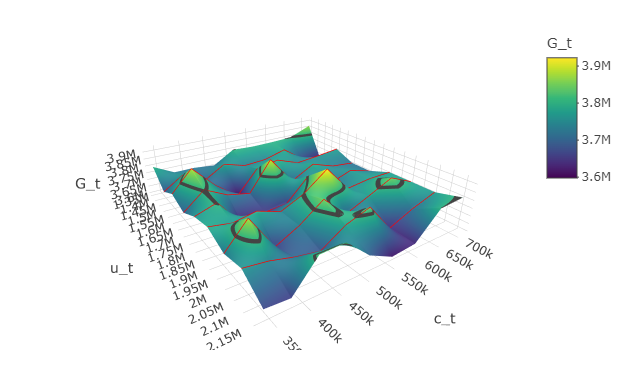
\includegraphics[width=5.20833in,height=\textheight,keepaspectratio]{fig-analisispdf.png}

}

\caption{Análisis de sensibilidad pre-pandemia para 90 semanas}

\end{figure}%

\subsection{Caso pos-pandemia}\label{caso-pos-pandemia}

De manera análoga a la metodología empleada con los datos
pre-pandémicos, para la simulación del modelo Crámer-Lundberg, con los
datos después de la pandemia se hizo uso de las medias de las
distribuciones de las ventas por día tomado como las ganancias
acumuladas, y se estimó los parámetros de \(u\) y \(c\).

\subsubsection{Modelo de Cramér-Lundberg simulado en R con datos reales
de las ventas por día de la
empresa}\label{modelo-de-cramuxe9r-lundberg-simulado-en-r-con-datos-reales-de-las-ventas-por-duxeda-de-la-empresa}

En la (Figura~\ref{fig-fig-trayectoria2pdf}) se muestra la trayectoria
del modelo bajo los supuestos del modelo modificado, el proceso comienza
con \(t = 14\), que son las \(14\) semanas de las ventas registradas por
día después del cierre pandémico, con un capital inicial de
\(u= 1759629\), una tasa de \(c= 0.29\). Los montos de las ganancias
tienen todas distribución normal (\(N\)).

Como se muestra en la siguiente tabla:

\begin{longtable}[]{@{}lll@{}}
\toprule\noalign{}
DÍA & MEDIA & VARIANZA \\
\midrule\noalign{}
\endhead
\bottomrule\noalign{}
\endlastfoot
Domingo & \(101919.050\) & \(118310761\) \\
Lunes & \(42338.847\) & \(145157292\) \\
Martes & \(41751.747\) & \(32342310\) \\
Miércoles & \(43243.143\) & \(1869969417\) \\
Jueves & \(43010.307\) & \(59936845\) \\
Viernes & \(61191.30\) & \(51883051\) \\
Sábado & \(85684.058\) & \(70079652\) \\
\end{longtable}

El código que genera la trayectoria es el siguiente:

\begin{Shaded}
\begin{Highlighting}[]
\FunctionTok{library}\NormalTok{(dplyr) }\CommentTok{\# librería para poder renombrar }
\CommentTok{\#las cabeceras de los dataframes}
\CommentTok{\#Parámetros}
\FunctionTok{set.seed}\NormalTok{(}\DecValTok{13}\NormalTok{) }\CommentTok{\#semilla fija}
\NormalTok{u }\OtherTok{=} \DecValTok{1759629} \CommentTok{\#surplus(capital inicial de salvamento)}
\CommentTok{\#Es un estimado a partir de la media de las ganancias por semana, }
\CommentTok{\#multiplicado por 10/3, }
\CommentTok{\#siendo una proporción para evitar la ruina}
\CommentTok{\# u (sum(medias))*(10/3)}
\NormalTok{c }\OtherTok{=}\NormalTok{ (}\FloatTok{0.29}\SpecialCharTok{*}\NormalTok{u) }\CommentTok{\#prima de pago cada tiempo t. c = 0.5*u}
\NormalTok{lambda\_Nt }\OtherTok{=} \FloatTok{0.5}
\CommentTok{\#lambda\_Xi = 3}
\NormalTok{t\_final }\OtherTok{=} \DecValTok{14}
\CommentTok{\# S(t) = \textbackslash{}sum\_\{i=1\}\^{}\{N(t)\}X\_i}
\CommentTok{\#donde N(t)\textasciitilde{} Poisson (lambda*t)}
\CommentTok{\# X\_i \textasciitilde{} exponencial (lambda\_Xi)}
\CommentTok{\#CL = REPRESENTA EL MODELO DE CRAMER LUNDBERG}
\CommentTok{\#Simulación de trayectoria de CL\_t, cuando t \textless{} t\_final.}
\NormalTok{trayectoria\_CLt\_post\_pandemia }\OtherTok{\textless{}{-}} \ControlFlowTok{function}\NormalTok{(u, c, lambda\_Nt, t\_final)}
\NormalTok{\{}
\NormalTok{  tiempo }\OtherTok{\textless{}{-}} \FunctionTok{c}\NormalTok{(}\DecValTok{0}\NormalTok{)}
\NormalTok{  Cramer\_trayectoria }\OtherTok{\textless{}{-}} \FunctionTok{c}\NormalTok{(u)}
  \ControlFlowTok{while}\NormalTok{(tiempo[}\FunctionTok{length}\NormalTok{(tiempo)] }\SpecialCharTok{\textless{}}\NormalTok{ t\_final)}
\NormalTok{  \{}
\NormalTok{    tiempo\_llegada }\OtherTok{\textless{}{-}}\NormalTok{ (}\DecValTok{1}\NormalTok{)}\CommentTok{\#rexp(1, rate = lambda\_Nt)}
\NormalTok{    Y\_i }\OtherTok{\textless{}{-}}\NormalTok{  (}\FunctionTok{rnorm}\NormalTok{(}\DecValTok{1}\NormalTok{, }\AttributeTok{mean =} \FloatTok{101919.050}\NormalTok{ , }\AttributeTok{sd =} \FloatTok{10877.075}\NormalTok{)}\SpecialCharTok{+}
             \FunctionTok{rnorm}\NormalTok{(}\DecValTok{1}\NormalTok{, }\AttributeTok{mean =}  \FloatTok{39841.721}\NormalTok{ , }\AttributeTok{sd=} \FloatTok{7873.446}\NormalTok{)  }\SpecialCharTok{+} 
             \FunctionTok{rnorm}\NormalTok{(}\DecValTok{1}\NormalTok{, }\AttributeTok{mean =}   \FloatTok{41751.747}\NormalTok{, }\AttributeTok{sd =} \FloatTok{5687.030}\NormalTok{) }\SpecialCharTok{+} 
             \FunctionTok{rnorm}\NormalTok{(}\DecValTok{1}\NormalTok{, }\AttributeTok{mean =}   \FloatTok{43243.143}\NormalTok{, }\AttributeTok{sd =} \FloatTok{10517.841}\NormalTok{)}\SpecialCharTok{+} 
             \FunctionTok{rnorm}\NormalTok{(}\DecValTok{1}\NormalTok{, }\AttributeTok{mean =} \FloatTok{43010.307}\NormalTok{  , }\AttributeTok{sd =} \FloatTok{7741.889}\NormalTok{ )}\SpecialCharTok{+} 
             \FunctionTok{rnorm}\NormalTok{(}\DecValTok{1}\NormalTok{, }\AttributeTok{mean =} \FloatTok{61191.300}\NormalTok{  , }\AttributeTok{sd =} \FloatTok{7202.989}\NormalTok{) }\SpecialCharTok{+} 
             \FunctionTok{rnorm}\NormalTok{(}\DecValTok{1}\NormalTok{, }\AttributeTok{mean =}  \FloatTok{85684.058}\NormalTok{ , }\AttributeTok{sd =} \FloatTok{8371.359}\NormalTok{ ) ) }
\NormalTok{tiempo }\OtherTok{\textless{}{-}} \FunctionTok{c}\NormalTok{(tiempo, tiempo[}\FunctionTok{length}\NormalTok{(tiempo)] }\SpecialCharTok{+}
\NormalTok{              tiempo\_llegada,tiempo[}\FunctionTok{length}\NormalTok{(tiempo)] }\SpecialCharTok{+}
\NormalTok{              tiempo\_llegada ) }
\NormalTok{Cramer\_trayectoria }\OtherTok{\textless{}{-}} \FunctionTok{c}\NormalTok{(Cramer\_trayectoria,}
\NormalTok{Cramer\_trayectoria[}\FunctionTok{length}\NormalTok{(Cramer\_trayectoria)] }\SpecialCharTok{{-}}
\NormalTok{  c}\SpecialCharTok{*}\NormalTok{tiempo\_llegada, }
\NormalTok{Cramer\_trayectoria[}\FunctionTok{length}\NormalTok{(Cramer\_trayectoria)] }\SpecialCharTok{{-}}
\NormalTok{  c}\SpecialCharTok{*}\NormalTok{tiempo\_llegada }\SpecialCharTok{+}\NormalTok{  Y\_i )}
\NormalTok{  \}}
\NormalTok{  df\_post\_pandemia }\OtherTok{\textless{}{-}} \FunctionTok{data.frame}\NormalTok{(tiempo, Cramer\_trayectoria)}
\NormalTok{df\_trayectoria\_post\_pandemia }\OtherTok{\textless{}{-}} \FunctionTok{data.frame}\NormalTok{(df\_post\_pandemia}\SpecialCharTok{\%\textgreater{}\%} 
                                        \FunctionTok{rename}\NormalTok{(}\AttributeTok{Tiempo =}\NormalTok{ tiempo,}
                                        \AttributeTok{Ct =}\NormalTok{ Cramer\_trayectoria))}
  \FunctionTok{return}\NormalTok{(df\_trayectoria\_post\_pandemia)}
\NormalTok{\}}
\NormalTok{trayectoria\_post\_pandemia }\OtherTok{\textless{}{-}} \FunctionTok{trayectoria\_CLt\_post\_pandemia}\NormalTok{(u,c,}
\NormalTok{                                              lambda\_Nt,t\_final)}


\FunctionTok{library}\NormalTok{(plotly)}
\NormalTok{fig\_tr2 }\OtherTok{\textless{}{-}} \FunctionTok{plot\_ly}\NormalTok{(trayectoria\_post\_pandemia, }\AttributeTok{x =} \SpecialCharTok{\textasciitilde{}}\NormalTok{Tiempo, }
                                              \AttributeTok{y =} \SpecialCharTok{\textasciitilde{}}\NormalTok{Ct, }
          \AttributeTok{name =} \StringTok{"Ganancias: G(t)"}\NormalTok{,}
          \AttributeTok{type =} \StringTok{"scatter"}\NormalTok{, }\AttributeTok{mode =} \StringTok{"lines"}\NormalTok{)}

\NormalTok{fig\_tr2 }\OtherTok{\textless{}{-}}\NormalTok{ fig\_tr2 }\SpecialCharTok{\%\textgreater{}\%} \FunctionTok{add\_trace}\NormalTok{(}\AttributeTok{x =} \SpecialCharTok{\textasciitilde{}}\NormalTok{Tiempo, }\AttributeTok{y =}\NormalTok{ u,}
        \AttributeTok{name =} \StringTok{"Capital inicial: u"}\NormalTok{, }
        \AttributeTok{type =} \StringTok{"scatter"}\NormalTok{, }\AttributeTok{mode =} \StringTok{"lines"}\NormalTok{)}
\NormalTok{fig\_tr2}
\end{Highlighting}
\end{Shaded}

\begin{figure}

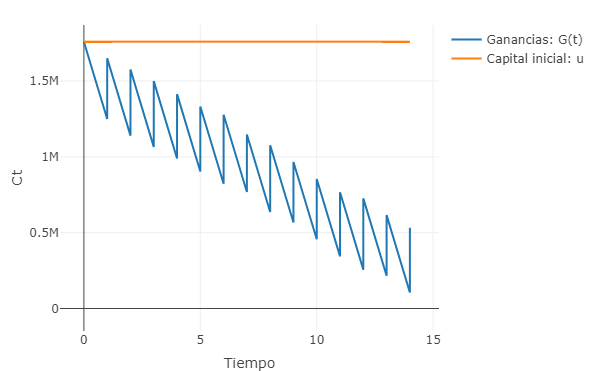
\includegraphics[width=6.25in,height=\textheight,keepaspectratio]{trayectoria2pdf.png}

\caption{\label{fig-fig-trayectoria2pdf}Trayectoria de pérdidas del
proceso de evolución modificado de Cramér-Lundberg después de la
pandemia}

\end{figure}%

Se emplean los mismos parámetros obtenidos en el periodo de tiempo pre
pandemia del modelo modificado donde se observa una completa ruina al
alcanzar \(17\) semanas.

\begin{Shaded}
\begin{Highlighting}[]
\FunctionTok{library}\NormalTok{(dplyr) }\CommentTok{\# librería para poder renombrar }
\CommentTok{\# las cabeceras de los dataframes}

\CommentTok{\#Parámetros}
\FunctionTok{set.seed}\NormalTok{(}\DecValTok{13}\NormalTok{) }\CommentTok{\#semilla fija}
\NormalTok{u }\OtherTok{=} \DecValTok{1759629} \CommentTok{\#surplus(capital inicial de salvamento)}
\CommentTok{\#Es un estimado a partir de la media de las ganancias por semana, }
\CommentTok{\#multiplicado por 10/3, }
\CommentTok{\#siendo una proporción para evitar la ruina}
\CommentTok{\# u (sum(medias))*(10/3)}
\NormalTok{c }\OtherTok{=} \FloatTok{0.29}\SpecialCharTok{*}\NormalTok{u }\CommentTok{\#prima de pago cada tiempo t. c = 0.5*u}
\NormalTok{lambda\_Nt }\OtherTok{=} \FloatTok{0.5}
\CommentTok{\#lambda\_Xi = 3}
\NormalTok{t\_final }\OtherTok{=} \DecValTok{17}
\CommentTok{\# S(t) = \textbackslash{}sum\_\{i=1\}\^{}\{N(t)\}X\_i}
\CommentTok{\#donde N(t)\textasciitilde{} Poisson (lambda*t)}
\CommentTok{\# X\_i \textasciitilde{} exponencial (lambda\_Xi)}
\CommentTok{\#CL = REPRESENTA EL MODELO DE CRAMER LUNDBERG}
\CommentTok{\#Simulación de trayectoria de CL\_t, cuando t \textless{} t\_final.}
\NormalTok{trayectoria\_CLt\_post\_pandemia }\OtherTok{\textless{}{-}} \ControlFlowTok{function}\NormalTok{(u, c, lambda\_Nt, t\_final)}
\NormalTok{\{}
\NormalTok{  tiempo }\OtherTok{\textless{}{-}} \FunctionTok{c}\NormalTok{(}\DecValTok{0}\NormalTok{)}
\NormalTok{  Cramer\_trayectoria }\OtherTok{\textless{}{-}} \FunctionTok{c}\NormalTok{(u)}
  \ControlFlowTok{while}\NormalTok{(tiempo[}\FunctionTok{length}\NormalTok{(tiempo)] }\SpecialCharTok{\textless{}}\NormalTok{ t\_final)}
\NormalTok{  \{}
\NormalTok{    tiempo\_llegada }\OtherTok{\textless{}{-}}\NormalTok{ (}\DecValTok{1}\NormalTok{)}\CommentTok{\#rexp(1, rate = lambda\_Nt)}
\NormalTok{    Y\_i }\OtherTok{\textless{}{-}}\NormalTok{  (}\FunctionTok{rnorm}\NormalTok{(}\DecValTok{1}\NormalTok{, }\AttributeTok{mean =} \FloatTok{101919.050}\NormalTok{ , }\AttributeTok{sd =} \FloatTok{10877.075}\NormalTok{  ) }
\SpecialCharTok{+} \FunctionTok{rnorm}\NormalTok{(}\DecValTok{1}\NormalTok{, }\AttributeTok{mean =}  \FloatTok{39841.721}\NormalTok{ , }\AttributeTok{sd=} \FloatTok{7873.446} 
\NormalTok{    ) }\SpecialCharTok{+}  
\FunctionTok{rnorm}\NormalTok{(}\DecValTok{1}\NormalTok{, }\AttributeTok{mean =}   \FloatTok{41751.747}\NormalTok{, }\AttributeTok{sd =} \FloatTok{5687.030}\NormalTok{  ) }\SpecialCharTok{+} 
\FunctionTok{rnorm}\NormalTok{(}\DecValTok{1}\NormalTok{, }\AttributeTok{mean =}   \FloatTok{43243.143}\NormalTok{, }\AttributeTok{sd =} \FloatTok{10517.841}\NormalTok{ ) }\SpecialCharTok{+} 
\FunctionTok{rnorm}\NormalTok{(}\DecValTok{1}\NormalTok{, }\AttributeTok{mean =} \FloatTok{43010.307}\NormalTok{  , }\AttributeTok{sd =} \FloatTok{7741.889}\NormalTok{ ) }\SpecialCharTok{+} 
\FunctionTok{rnorm}\NormalTok{(}\DecValTok{1}\NormalTok{, }\AttributeTok{mean =} \FloatTok{61191.300}\NormalTok{  , }\AttributeTok{sd =} \FloatTok{7202.989}\NormalTok{) }\SpecialCharTok{+} 
\FunctionTok{rnorm}\NormalTok{(}\DecValTok{1}\NormalTok{, }\AttributeTok{mean =}  \FloatTok{85684.058}\NormalTok{ , }\AttributeTok{sd =} \FloatTok{8371.359}\NormalTok{ ) ) }
\NormalTok{    tiempo }\OtherTok{\textless{}{-}} \FunctionTok{c}\NormalTok{(tiempo, tiempo[}\FunctionTok{length}\NormalTok{(tiempo)] }
    \SpecialCharTok{+}\NormalTok{ tiempo\_llegada,tiempo[}\FunctionTok{length}\NormalTok{(tiempo)]}
    \SpecialCharTok{+}\NormalTok{ tiempo\_llegada ) }
\NormalTok{    Cramer\_trayectoria }\OtherTok{\textless{}{-}} \FunctionTok{c}\NormalTok{(Cramer\_trayectoria,}
\NormalTok{    Cramer\_trayectoria[}\FunctionTok{length}\NormalTok{(Cramer\_trayectoria)]}
    \SpecialCharTok{{-}}\NormalTok{ c}\SpecialCharTok{*}\NormalTok{tiempo\_llegada,}
\NormalTok{    Cramer\_trayectoria[}\FunctionTok{length}\NormalTok{(Cramer\_trayectoria)]}\SpecialCharTok{{-}}
\NormalTok{    c}\SpecialCharTok{*}\NormalTok{tiempo\_llegada }\SpecialCharTok{+}\NormalTok{  Y\_i )}
\NormalTok{  \}}
\NormalTok{  df\_post\_pandemia }\OtherTok{\textless{}{-}} \FunctionTok{data.frame}\NormalTok{(tiempo, Cramer\_trayectoria)}
\NormalTok{df\_trayectoria\_post\_pandemia }\OtherTok{\textless{}{-}} \FunctionTok{data.frame}\NormalTok{(df\_post\_pandemia}\SpecialCharTok{\%\textgreater{}\%}
                                        \FunctionTok{rename}\NormalTok{(}\AttributeTok{Tiempo =}\NormalTok{ tiempo,}
    \AttributeTok{Ct =}\NormalTok{ Cramer\_trayectoria))}
  \FunctionTok{return}\NormalTok{(df\_trayectoria\_post\_pandemia)}
\NormalTok{\}}
\NormalTok{trayectoria\_post\_pandemia }\OtherTok{\textless{}{-}} \FunctionTok{trayectoria\_CLt\_post\_pandemia}\NormalTok{(u,c,}
\NormalTok{                                            lambda\_Nt, t\_final )}

\FunctionTok{library}\NormalTok{(plotly)}
\NormalTok{fig\_tr3 }\OtherTok{\textless{}{-}} \FunctionTok{plot\_ly}\NormalTok{(trayectoria\_post\_pandemia, }\AttributeTok{x =} \SpecialCharTok{\textasciitilde{}}\NormalTok{Tiempo, }
                                              \AttributeTok{y =} \SpecialCharTok{\textasciitilde{}}\NormalTok{Ct,}
            \AttributeTok{name =} \StringTok{"Ganancias:G(t)"}\NormalTok{,}
            \AttributeTok{type =} \StringTok{"scatter"}\NormalTok{, }\AttributeTok{mode =} \StringTok{"lines"}\NormalTok{)}

\NormalTok{fig\_tr3 }\OtherTok{\textless{}{-}}\NormalTok{ fig\_tr3 }\SpecialCharTok{\%\textgreater{}\%} \FunctionTok{add\_trace}\NormalTok{(}\AttributeTok{x =} \SpecialCharTok{\textasciitilde{}}\NormalTok{Tiempo, }\AttributeTok{y =}\NormalTok{ u,}
           \AttributeTok{name =} \StringTok{"Capital inicial:u"}\NormalTok{, }
           \AttributeTok{type =} \StringTok{"scatter"}\NormalTok{, }\AttributeTok{mode =} \StringTok{"lines"}\NormalTok{)}
\NormalTok{fig\_tr3}
\end{Highlighting}
\end{Shaded}

\begin{figure}

\centering{

\pandocbounded{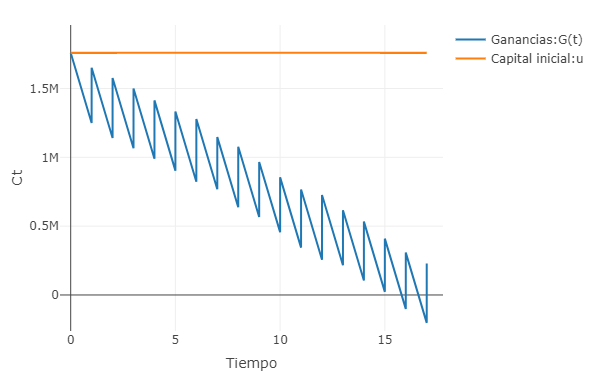
\includegraphics[keepaspectratio]{trayectoria3pdf.png}}

}

\caption{\label{fig-fig-trayectoria3pdf}Trayectoria del proceso de
evolución de las pérdidas en el modelo modificado de Cramér-Lundberg
después de la pandemia para 17 semanas.}

\end{figure}%

La evolución del proceso de pérdidas en el modelo modificado de
Cramér-Lundberg proporciona una herramienta más precisa y adaptable para
predecir y contrarrestar los impactos financieros negativos de la
empresa.

Se incorpora un factor adicional y ajuste que mejoran la simulación del
modelo, mediante la modificación del parámetro \(c\), reduciendo un
\(17\%\) la prima de pago, logrando sustentarse por más tiempo
estabilizando los ingresos, presentándose así los resultados mediante el
siguiente código.

\begin{Shaded}
\begin{Highlighting}[]
\FunctionTok{library}\NormalTok{(dplyr) }\CommentTok{\# libreráa para poder renombrar }
\CommentTok{\# las cabeceras de los dataframes}

\CommentTok{\#Parámetros}
\FunctionTok{set.seed}\NormalTok{(}\DecValTok{13}\NormalTok{) }\CommentTok{\#semilla fija}
\NormalTok{u }\OtherTok{=} \DecValTok{1759629} \CommentTok{\#surplus(capital inicial de salvamento)}
\CommentTok{\#Es un estimado a partir de la media de las ganancias por semana, }
\CommentTok{\#multiplicado por 10/3, }
\CommentTok{\#siendo una proporción para evitar la ruina}
\CommentTok{\# u (sum(medias))*(10/3)}
\NormalTok{c }\OtherTok{=}\NormalTok{ (}\FloatTok{0.29}\SpecialCharTok{*}\NormalTok{u)}\SpecialCharTok{*}\NormalTok{(}\FloatTok{0.83}\NormalTok{) }\CommentTok{\#prima de pago cada tiempo t. c = 0.5*u}
\NormalTok{lambda\_Nt }\OtherTok{=} \FloatTok{0.5}
\CommentTok{\#lambda\_Xi = 3}
\NormalTok{t\_final }\OtherTok{=} \DecValTok{14}
\CommentTok{\# S(t) = \textbackslash{}sum\_\{i=1\}\^{}\{N(t)\}X\_i}
\CommentTok{\#donde N(t)\textasciitilde{} Poisson (lambda*t)}
\CommentTok{\# X\_i \textasciitilde{} exponencial (lambda\_Xi)}
\CommentTok{\#CL = REPRESENTA EL MODELO DE CRAMER LUNDBERG}
\CommentTok{\#Simulación de trayectoria de CL\_t, cuando t \textless{} t\_final.}
\NormalTok{trayectoria\_CLt\_post\_pandemia }\OtherTok{\textless{}{-}} \ControlFlowTok{function}\NormalTok{(u, c, lambda\_Nt, t\_final)}
\NormalTok{\{}
\NormalTok{  tiempo }\OtherTok{\textless{}{-}} \FunctionTok{c}\NormalTok{(}\DecValTok{0}\NormalTok{)}
\NormalTok{  Cramer\_trayectoria }\OtherTok{\textless{}{-}} \FunctionTok{c}\NormalTok{(u)}
  \ControlFlowTok{while}\NormalTok{(tiempo[}\FunctionTok{length}\NormalTok{(tiempo)] }\SpecialCharTok{\textless{}}\NormalTok{ t\_final)}
\NormalTok{  \{}
\NormalTok{    tiempo\_llegada }\OtherTok{\textless{}{-}}\NormalTok{ (}\DecValTok{1}\NormalTok{)}\CommentTok{\#rexp(1, rate = lambda\_Nt)}
    
\NormalTok{    Y\_i }\OtherTok{\textless{}{-}}\NormalTok{  (}\FunctionTok{rnorm}\NormalTok{(}\DecValTok{1}\NormalTok{, }\AttributeTok{mean =} \FloatTok{101919.050}\NormalTok{ , }\AttributeTok{sd =} \FloatTok{10877.075}\NormalTok{) }\SpecialCharTok{+} 
            \FunctionTok{rnorm}\NormalTok{(}\DecValTok{1}\NormalTok{, }\AttributeTok{mean =}  \FloatTok{39841.721}\NormalTok{ , }\AttributeTok{sd=} \FloatTok{7873.446}\NormalTok{) }\SpecialCharTok{+}  
            \FunctionTok{rnorm}\NormalTok{(}\DecValTok{1}\NormalTok{, }\AttributeTok{mean =}   \FloatTok{41751.747}\NormalTok{, }\AttributeTok{sd =} \FloatTok{5687.030}\NormalTok{) }\SpecialCharTok{+} 
            \FunctionTok{rnorm}\NormalTok{(}\DecValTok{1}\NormalTok{, }\AttributeTok{mean =}   \FloatTok{43243.143}\NormalTok{, }\AttributeTok{sd =} \FloatTok{10517.841}\NormalTok{) }\SpecialCharTok{+} 
            \FunctionTok{rnorm}\NormalTok{(}\DecValTok{1}\NormalTok{, }\AttributeTok{mean =} \FloatTok{43010.307}\NormalTok{  , }\AttributeTok{sd =} \FloatTok{7741.889}\NormalTok{) }\SpecialCharTok{+} 
            \FunctionTok{rnorm}\NormalTok{(}\DecValTok{1}\NormalTok{, }\AttributeTok{mean =} \FloatTok{61191.300}\NormalTok{  , }\AttributeTok{sd =} \FloatTok{7202.989}\NormalTok{) }\SpecialCharTok{+} 
            \FunctionTok{rnorm}\NormalTok{(}\DecValTok{1}\NormalTok{, }\AttributeTok{mean =}  \FloatTok{85684.058}\NormalTok{ , }\AttributeTok{sd =} \FloatTok{8371.359}\NormalTok{ )) }
\NormalTok{    tiempo }\OtherTok{\textless{}{-}} \FunctionTok{c}\NormalTok{(tiempo, tiempo[}\FunctionTok{length}\NormalTok{(tiempo)] }\SpecialCharTok{+} 
\NormalTok{                tiempo\_llegada,tiempo[}\FunctionTok{length}\NormalTok{(tiempo)] }\SpecialCharTok{+} 
\NormalTok{                tiempo\_llegada ) }
\NormalTok{    Cramer\_trayectoria }\OtherTok{\textless{}{-}} \FunctionTok{c}\NormalTok{(Cramer\_trayectoria,}
\NormalTok{                    Cramer\_trayectoria[}\FunctionTok{length}\NormalTok{(Cramer\_trayectoria)]}\SpecialCharTok{{-}}
\NormalTok{                          c}\SpecialCharTok{*}\NormalTok{tiempo\_llegada, }
\NormalTok{                    Cramer\_trayectoria[}\FunctionTok{length}\NormalTok{(Cramer\_trayectoria)]}\SpecialCharTok{{-}} 
\NormalTok{                            c}\SpecialCharTok{*}\NormalTok{tiempo\_llegada }\SpecialCharTok{+}\NormalTok{ Y\_i )}
\NormalTok{  \}}
\NormalTok{  df\_post\_pandemia }\OtherTok{\textless{}{-}} \FunctionTok{data.frame}\NormalTok{(tiempo, Cramer\_trayectoria)}
\NormalTok{  df\_trayectoria\_post\_pandemia }\OtherTok{\textless{}{-}} \FunctionTok{data.frame}\NormalTok{(df\_post\_pandemia}\SpecialCharTok{\%\textgreater{}\%} 
                                          \FunctionTok{rename}\NormalTok{(}\AttributeTok{Tiempo =}\NormalTok{ tiempo, }
                                          \AttributeTok{Ct =}\NormalTok{ Cramer\_trayectoria))}
  \FunctionTok{return}\NormalTok{(df\_trayectoria\_post\_pandemia)}
\NormalTok{\}}
\NormalTok{trayectoria\_post\_pandemia }\OtherTok{\textless{}{-}} \FunctionTok{trayectoria\_CLt\_post\_pandemia}\NormalTok{(u,c,}
\NormalTok{                                            lambda\_Nt, t\_final )}


\FunctionTok{library}\NormalTok{(plotly)}

\NormalTok{fig\_tr4 }\OtherTok{\textless{}{-}} \FunctionTok{plot\_ly}\NormalTok{(trayectoria\_post\_pandemia, }\AttributeTok{x =} \SpecialCharTok{\textasciitilde{}}\NormalTok{Tiempo, }
                   \AttributeTok{y =} \SpecialCharTok{\textasciitilde{}}\NormalTok{Ct, }
         \AttributeTok{name =} \StringTok{"Ganancias: G(t)"}\NormalTok{,}
         \AttributeTok{type =} \StringTok{"scatter"}\NormalTok{, }\AttributeTok{mode =} \StringTok{"lines"}\NormalTok{)}

\NormalTok{fig\_tr4 }\OtherTok{\textless{}{-}}\NormalTok{ fig\_tr4 }\SpecialCharTok{\%\textgreater{}\%} \FunctionTok{add\_trace}\NormalTok{(}\AttributeTok{x =} \SpecialCharTok{\textasciitilde{}}\NormalTok{Tiempo, }\AttributeTok{y =}\NormalTok{ u,}
        \AttributeTok{name =} \StringTok{"Capital inicial: u"}\NormalTok{, }
        \AttributeTok{type =} \StringTok{"scatter"}\NormalTok{, }\AttributeTok{mode =} \StringTok{"lines"}\NormalTok{)}
\NormalTok{fig\_tr4}
\end{Highlighting}
\end{Shaded}

\begin{figure}

\centering{

\pandocbounded{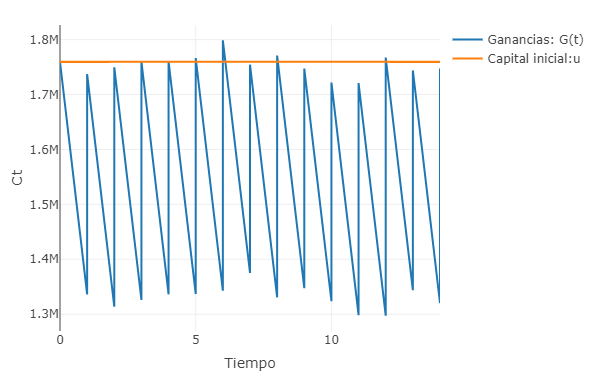
\includegraphics[keepaspectratio]{trayectoria4pdf.png}}

}

\caption{\label{fig-fig-trayectoria4pdf}Trayectoria del proceso de
pérdidas generadas por el modelo de Cramér-Lundberg después de la
pandemia con una reducción de los costos al 17\%.}

\end{figure}%

\subsubsection{Simulación de la probabilidad de
ruina}\label{simulaciuxf3n-de-la-probabilidad-de-ruina-1}

Al igual que para el periodo antes de la pandemia se analizó el periodo
pos-pandemia la semana en el que \(G(t)\leq u\) y cuando \(G(t)\leq0\),
haciendo la comparación con la tasa de interés de \(0.8\%\) anual en una
cuenta de ahorro de una entidad bancaria por la misma inversión del
capital inicial \(u\), para este periodo tomamos \(t = 14\), es decir
los datos registrados hasta las \(14\) semanas después de pandemia donde
la tasa es de \(0.0233.\)

El código para calcular la probabilidad de las ganancias finales bajas
es el siguiente:

\begin{Shaded}
\begin{Highlighting}[]
\FunctionTok{library}\NormalTok{(dplyr) }\CommentTok{\# librería para poder renombrar las }
\CommentTok{\# cabeceras de los dataframes}

\CommentTok{\#Parámetros}
\FunctionTok{set.seed}\NormalTok{(}\DecValTok{13}\NormalTok{) }\CommentTok{\#semilla fija}
\NormalTok{u }\OtherTok{=} \DecValTok{1759629} \CommentTok{\#surplus(capital inicial de salvamento)}
\CommentTok{\#Es un estimado a partir de la media de las ganancias por semana, }
\CommentTok{\#multiplicado por 10/3, }
\CommentTok{\#siendo una proporción para evitar la ruina}
\CommentTok{\# u (sum(medias))*(10/3)}
\NormalTok{c }\OtherTok{=} \FloatTok{0.29}\SpecialCharTok{*}\NormalTok{u }\CommentTok{\#prima de pago cada tiempo t. c = 0.5*u}
\NormalTok{lambda\_Nt }\OtherTok{=} \FloatTok{0.5}
\CommentTok{\#lambda\_Xi = 3}
\NormalTok{t\_final }\OtherTok{=} \DecValTok{14}
\NormalTok{mu }\OtherTok{=} \DecValTok{1} \CommentTok{\#tiempos entre llegadas constantes}
\CommentTok{\# S(t) = \textbackslash{}sum\_\{i=1\}\^{}\{N(t)\}X\_i}
\CommentTok{\#donde N(t)\textasciitilde{} Poisson (lambda*t)}
\CommentTok{\# X\_i \textasciitilde{} exponencial (lambda\_Xi)}
\CommentTok{\#CL = REPRESENTA EL MODELO DE CRAMER LUNDBERG}
\CommentTok{\#Simulación de trayectoria de CL\_t, cuando t \textless{} t\_final.}
\NormalTok{trayectoria\_CLt\_post\_pandemia }\OtherTok{\textless{}{-}} \ControlFlowTok{function}\NormalTok{(u, c, lambda\_Nt, t\_final)}
\NormalTok{\{}
\NormalTok{  tiempo }\OtherTok{\textless{}{-}} \FunctionTok{c}\NormalTok{(}\DecValTok{0}\NormalTok{)}
\NormalTok{  Cramer\_trayectoria }\OtherTok{\textless{}{-}} \FunctionTok{c}\NormalTok{(u)}
  \ControlFlowTok{while}\NormalTok{(tiempo[}\FunctionTok{length}\NormalTok{(tiempo)] }\SpecialCharTok{\textless{}}\NormalTok{ t\_final)}
\NormalTok{  \{}
    \CommentTok{\#tiempo\_llegada \textless{}{-} rexp(1, rate = lambda\_Nt)}
\NormalTok{    tiempo\_llegada }\OtherTok{\textless{}{-}}\NormalTok{ (}\DecValTok{1}\NormalTok{) }
\CommentTok{\#Suponiendo los tiempos entre llegadas constantes \textbackslash{}mu = 1}
\NormalTok{    Y\_i }\OtherTok{\textless{}{-}}\NormalTok{  (}\FunctionTok{rnorm}\NormalTok{(}\DecValTok{1}\NormalTok{, }\AttributeTok{mean =} \FloatTok{101919.050}\NormalTok{ , }\AttributeTok{sd =} \FloatTok{10877.075}\NormalTok{   ) }
              \SpecialCharTok{+} \FunctionTok{rnorm}\NormalTok{(}\DecValTok{1}\NormalTok{, }\AttributeTok{mean =}  \FloatTok{39841.721}\NormalTok{ , }\AttributeTok{sd=} \FloatTok{7873.446}\NormalTok{  ) }
              \SpecialCharTok{+} \FunctionTok{rnorm}\NormalTok{(}\DecValTok{1}\NormalTok{, }\AttributeTok{mean =}   \FloatTok{41751.747}\NormalTok{, }\AttributeTok{sd =} \FloatTok{5687.030}\NormalTok{ ) }
              \SpecialCharTok{+} \FunctionTok{rnorm}\NormalTok{(}\DecValTok{1}\NormalTok{, }\AttributeTok{mean =}   \FloatTok{43243.143}\NormalTok{, }\AttributeTok{sd =} \FloatTok{10517.841}\NormalTok{) }
              \SpecialCharTok{+} \FunctionTok{rnorm}\NormalTok{(}\DecValTok{1}\NormalTok{, }\AttributeTok{mean =} \FloatTok{43010.307}\NormalTok{  , }\AttributeTok{sd =} \FloatTok{7741.889}\NormalTok{ ) }
              \SpecialCharTok{+} \FunctionTok{rnorm}\NormalTok{(}\DecValTok{1}\NormalTok{, }\AttributeTok{mean =} \FloatTok{61191.300}\NormalTok{  , }\AttributeTok{sd =} \FloatTok{7202.989}\NormalTok{ ) }
              \SpecialCharTok{+} \FunctionTok{rnorm}\NormalTok{(}\DecValTok{1}\NormalTok{, }\AttributeTok{mean =}  \FloatTok{85684.058}\NormalTok{ , }\AttributeTok{sd =} \FloatTok{8371.359}\NormalTok{)) }
\NormalTok{    tiempo }\OtherTok{\textless{}{-}} \FunctionTok{c}\NormalTok{(tiempo, tiempo[}\FunctionTok{length}\NormalTok{(tiempo)] }\SpecialCharTok{+} 
\NormalTok{                  tiempo\_llegada,tiempo[}\FunctionTok{length}\NormalTok{(tiempo)]}\SpecialCharTok{+} 
\NormalTok{                  tiempo\_llegada) }
\NormalTok{    Cramer\_trayectoria }\OtherTok{\textless{}{-}} \FunctionTok{c}\NormalTok{(Cramer\_trayectoria,}
\NormalTok{    Cramer\_trayectoria[}\FunctionTok{length}\NormalTok{(Cramer\_trayectoria)] }\SpecialCharTok{{-}} 
\NormalTok{      c}\SpecialCharTok{*}\NormalTok{tiempo\_llegada, }
\NormalTok{    Cramer\_trayectoria[}\FunctionTok{length}\NormalTok{(Cramer\_trayectoria)]}\SpecialCharTok{{-}} 
\NormalTok{      c}\SpecialCharTok{*}\NormalTok{tiempo\_llegada }\SpecialCharTok{+}\NormalTok{  Y\_i )}
    \ControlFlowTok{if}\NormalTok{(Cramer\_trayectoria[}\FunctionTok{length}\NormalTok{(Cramer\_trayectoria)] }\SpecialCharTok{\textless{}} \DecValTok{0}\NormalTok{)\{}
\NormalTok{      ruina }\OtherTok{=} \DecValTok{1}
\NormalTok{    \}}
    \ControlFlowTok{else}\NormalTok{\{}
\NormalTok{      ruina }\OtherTok{=} \DecValTok{0}
\NormalTok{    \}}
\NormalTok{  \}}
\CommentTok{\# 1.08*u es la ganancia inferior a la de un tasa de }
\CommentTok{\# un título financiero  para el año 2018}
  
  \ControlFlowTok{if}\NormalTok{(Cramer\_trayectoria[}\FunctionTok{length}\NormalTok{(Cramer\_trayectoria)] }\SpecialCharTok{\textless{}}\NormalTok{ (}\DecValTok{1} \SpecialCharTok{+}\NormalTok{ (}\DecValTok{14}\SpecialCharTok{*}\FloatTok{0.08}\NormalTok{)}\SpecialCharTok{/}\DecValTok{48}\NormalTok{)}\SpecialCharTok{*}\NormalTok{u) \{}
\NormalTok{    ganancia\_no\_deseada }\OtherTok{=} \DecValTok{1}
    
\NormalTok{  \} }
  \ControlFlowTok{else}\NormalTok{\{}
\NormalTok{    ganancia\_no\_deseada }\OtherTok{=} \DecValTok{0}
\NormalTok{  \}}
\NormalTok{  df\_post\_pandemia }\OtherTok{\textless{}{-}} \FunctionTok{data.frame}\NormalTok{(tiempo, Cramer\_trayectoria)}
\NormalTok{  df\_trayectoria\_post\_pandemia }\OtherTok{\textless{}{-}} \FunctionTok{data.frame}\NormalTok{(df\_post\_pandemia}\SpecialCharTok{\%\textgreater{}\%} 
                                  \FunctionTok{rename}\NormalTok{(}\AttributeTok{Tiempo =}\NormalTok{ tiempo,}
                                         \AttributeTok{Ct =}\NormalTok{ Cramer\_trayectoria))}
\NormalTok{  salida }\OtherTok{\textless{}{-}} \FunctionTok{c}\NormalTok{(ruina, ganancia\_no\_deseada)}
  \FunctionTok{return}\NormalTok{(salida)}
  
\NormalTok{\}}
\NormalTok{trayectoria\_post\_pandemia }\OtherTok{\textless{}{-}} \FunctionTok{trayectoria\_CLt\_post\_pandemia}\NormalTok{(u,c,}
\NormalTok{                                            lambda\_Nt, t\_final )}
\CommentTok{\#Método de monte carlo para estimar la probabilidad de ruina}
\NormalTok{n\_replicaciones }\OtherTok{=} \DecValTok{100}
\NormalTok{r\_baja\_ganancia\_post\_pandemia }\OtherTok{\textless{}{-}} \FunctionTok{replicate}\NormalTok{(n\_replicaciones,}
                          \FunctionTok{trayectoria\_CLt\_post\_pandemia}\NormalTok{(u, c, }
\NormalTok{                                         lambda\_Nt, t\_final)[}\DecValTok{2}\NormalTok{])}
\NormalTok{r\_baja\_ganancia\_post\_pandemia }
\NormalTok{prob\_baja\_ganancia\_post\_pandemia }\OtherTok{\textless{}{-}} \FunctionTok{sum}\NormalTok{(r\_baja\_ganancia\_post\_pandemia }\SpecialCharTok{\textgreater{}}\DecValTok{0}\NormalTok{)}\SpecialCharTok{/}
\NormalTok{n\_replicaciones}
\NormalTok{prob\_baja\_ganancia\_post\_pandemia}
\end{Highlighting}
\end{Shaded}

Claramente la probabilidad de las ganancias bajas de la evolución de
\(G(t)\) después de la pandemia es \(1\), pues como se muestra en la
Figura~\ref{fig-fig-trayectoria2pdf} todas las ventas registradas están
por debajo del capital inicial lo que significa la sustentabilidad de la
franquicia es baja y proyecta una ruina total en un tiempo de corto
plazo.

\begin{verbatim}
[1] 1
\end{verbatim}

El código para calcular la probabilidad de las ganancias finales bajas
durante las \(17\) semanas es el siguiente:

\begin{Shaded}
\begin{Highlighting}[]
\FunctionTok{library}\NormalTok{(dplyr) }\CommentTok{\# librería para poder renombrar }
\CommentTok{\#las cabeceras de los dataframes}

\CommentTok{\#Parámetros}
\FunctionTok{set.seed}\NormalTok{(}\DecValTok{13}\NormalTok{) }\CommentTok{\#semilla fija}
\NormalTok{u }\OtherTok{=} \DecValTok{1759629} \CommentTok{\#surplus(capital inicial de salvamento)}
\CommentTok{\#Es un estimado a partir de la media de las ganancias por semana, }
\CommentTok{\#multiplicado por 10/3, }
\CommentTok{\#siendo una proporción para evitar la ruina}
\CommentTok{\# u (sum(medias))*(10/3)}
\NormalTok{c }\OtherTok{=} \FloatTok{0.29}\SpecialCharTok{*}\NormalTok{u }\CommentTok{\#prima de pago cada tiempo t. c = 0.5*u}
\NormalTok{lambda\_Nt }\OtherTok{=} \FloatTok{0.5}
\CommentTok{\#lambda\_Xi = 3}
\NormalTok{t\_final }\OtherTok{=} \DecValTok{17}
\NormalTok{mu }\OtherTok{=} \DecValTok{1} \CommentTok{\#tiempos entre llegadas constantes}
\CommentTok{\#df\_media \textless{}{-} data.frame(df\_media\%\textgreater{}\% rename(tiempos = Tiempo ,}
\CommentTok{\#media\_trayectoria = cramer\_media)}
\CommentTok{\# S(t) = \textbackslash{}sum\_\{i=1\}\^{}\{N(t)\}X\_i}
\CommentTok{\#donde N(t)\textasciitilde{} Poisson (lambda*t)}
\CommentTok{\# X\_i \textasciitilde{} exponencial (lambda\_Xi)}
\CommentTok{\#CL = REPRESENTA EL MODELO DE CRAMER LUNDBERG}
\CommentTok{\#Simulación de trayectoria de CL\_t, cuando t \textless{} t\_final.}
\NormalTok{trayectoria\_CLt\_post\_pandemia }\OtherTok{\textless{}{-}} \ControlFlowTok{function}\NormalTok{(u, c, lambda\_Nt, t\_final)}
\NormalTok{\{}
\NormalTok{  tiempo }\OtherTok{\textless{}{-}} \FunctionTok{c}\NormalTok{(}\DecValTok{0}\NormalTok{)}
\NormalTok{  Cramer\_trayectoria }\OtherTok{\textless{}{-}} \FunctionTok{c}\NormalTok{(u)}
  \ControlFlowTok{while}\NormalTok{(tiempo[}\FunctionTok{length}\NormalTok{(tiempo)] }\SpecialCharTok{\textless{}}\NormalTok{ t\_final)}
\NormalTok{  \{}
    \CommentTok{\#tiempo\_llegada \textless{}{-} rexp(1, rate = lambda\_Nt)}
\NormalTok{    tiempo\_llegada }\OtherTok{\textless{}{-}}\NormalTok{ (}\DecValTok{1}\NormalTok{) }
\CommentTok{\#Suponiendo los tiempos entre llegadas constantes \textbackslash{}mu = 1}
\NormalTok{    Y\_i }\OtherTok{\textless{}{-}}\NormalTok{  (}\FunctionTok{rnorm}\NormalTok{(}\DecValTok{1}\NormalTok{, }\AttributeTok{mean =} \FloatTok{101919.050}\NormalTok{ , }\AttributeTok{sd =} \FloatTok{10877.075}\NormalTok{)}\SpecialCharTok{+} 
              \FunctionTok{rnorm}\NormalTok{(}\DecValTok{1}\NormalTok{, }\AttributeTok{mean =}  \FloatTok{39841.721}\NormalTok{ , }\AttributeTok{sd=} \FloatTok{7873.446}\NormalTok{) }\SpecialCharTok{+} 
              \FunctionTok{rnorm}\NormalTok{(}\DecValTok{1}\NormalTok{, }\AttributeTok{mean =}   \FloatTok{41751.747}\NormalTok{, }\AttributeTok{sd =} \FloatTok{5687.030}\NormalTok{)}\SpecialCharTok{+} 
              \FunctionTok{rnorm}\NormalTok{(}\DecValTok{1}\NormalTok{, }\AttributeTok{mean =}   \FloatTok{43243.143}\NormalTok{, }\AttributeTok{sd =} \FloatTok{10517.841}\NormalTok{)}\SpecialCharTok{+} 
              \FunctionTok{rnorm}\NormalTok{(}\DecValTok{1}\NormalTok{, }\AttributeTok{mean =} \FloatTok{43010.307}\NormalTok{  , }\AttributeTok{sd =} \FloatTok{7741.889}\NormalTok{)}\SpecialCharTok{+} 
              \FunctionTok{rnorm}\NormalTok{(}\DecValTok{1}\NormalTok{, }\AttributeTok{mean =} \FloatTok{61191.300}\NormalTok{  , }\AttributeTok{sd =} \FloatTok{7202.989}\NormalTok{)}\SpecialCharTok{+} 
              \FunctionTok{rnorm}\NormalTok{(}\DecValTok{1}\NormalTok{, }\AttributeTok{mean =}  \FloatTok{85684.058}\NormalTok{ , }\AttributeTok{sd =} \FloatTok{8371.359}\NormalTok{ )) }
\NormalTok{    tiempo }\OtherTok{\textless{}{-}} \FunctionTok{c}\NormalTok{(tiempo, tiempo[}\FunctionTok{length}\NormalTok{(tiempo)]}\SpecialCharTok{+} 
\NormalTok{                  tiempo\_llegada,tiempo[}\FunctionTok{length}\NormalTok{(tiempo)]}\SpecialCharTok{+} 
\NormalTok{                  tiempo\_llegada ) }
\NormalTok{    Cramer\_trayectoria }\OtherTok{\textless{}{-}} \FunctionTok{c}\NormalTok{(Cramer\_trayectoria,}
\NormalTok{                      Cramer\_trayectoria[}\FunctionTok{length}\NormalTok{(Cramer\_trayectoria)]}\SpecialCharTok{{-}}
\NormalTok{                      c}\SpecialCharTok{*}\NormalTok{tiempo\_llegada, }
\NormalTok{                      Cramer\_trayectoria[}\FunctionTok{length}\NormalTok{(Cramer\_trayectoria)]}\SpecialCharTok{{-}} 
\NormalTok{                      c}\SpecialCharTok{*}\NormalTok{tiempo\_llegada }\SpecialCharTok{+}\NormalTok{  Y\_i )}
    \ControlFlowTok{if}\NormalTok{(Cramer\_trayectoria[}\FunctionTok{length}\NormalTok{(Cramer\_trayectoria)] }\SpecialCharTok{\textless{}} \DecValTok{0}\NormalTok{)\{}
\NormalTok{      ruina }\OtherTok{=} \DecValTok{1}
\NormalTok{    \}}
    \ControlFlowTok{else}\NormalTok{\{}
\NormalTok{      ruina }\OtherTok{=} \DecValTok{0}
\NormalTok{    \}}
\NormalTok{  \}}
\CommentTok{\# 1.08*u es la ganancia inferior a la de un tasa de }
\CommentTok{\# un título financieropara el año 2018}
  \ControlFlowTok{if}\NormalTok{(Cramer\_trayectoria[}\FunctionTok{length}\NormalTok{(Cramer\_trayectoria)] }\SpecialCharTok{\textless{}}\NormalTok{ (}\DecValTok{1} \SpecialCharTok{+}\NormalTok{ (}\DecValTok{17}\SpecialCharTok{*}\FloatTok{0.08}\NormalTok{)}\SpecialCharTok{/}\DecValTok{48}\NormalTok{)}\SpecialCharTok{*}\NormalTok{u) \{}
\NormalTok{    ganancia\_no\_deseada }\OtherTok{=} \DecValTok{1}
    
\NormalTok{  \} }
  \ControlFlowTok{else}\NormalTok{\{}
\NormalTok{    ganancia\_no\_deseada }\OtherTok{=} \DecValTok{0}
\NormalTok{  \}}
\NormalTok{  df\_post\_pandemia }\OtherTok{\textless{}{-}} \FunctionTok{data.frame}\NormalTok{(tiempo, Cramer\_trayectoria)}
\NormalTok{  df\_trayectoria\_post\_pandemia }\OtherTok{\textless{}{-}} \FunctionTok{data.frame}\NormalTok{(df\_post\_pandemia}\SpecialCharTok{\%\textgreater{}\%}
                                            \FunctionTok{rename}\NormalTok{(}\AttributeTok{Tiempo =}\NormalTok{ tiempo, }
                                            \AttributeTok{Ct =}\NormalTok{ Cramer\_trayectoria))}
\NormalTok{  salida }\OtherTok{\textless{}{-}} \FunctionTok{c}\NormalTok{(ruina, ganancia\_no\_deseada)}
  \FunctionTok{return}\NormalTok{(salida)}
  
\NormalTok{\}}
\NormalTok{trayectoria\_post\_pandemia }\OtherTok{\textless{}{-}} \FunctionTok{trayectoria\_CLt\_post\_pandemia}\NormalTok{(u,c,}
\NormalTok{                                            lambda\_Nt, t\_final )}
\CommentTok{\#Método de monte carlo para estimar la probabilidad de ruina}
\NormalTok{n\_replicaciones }\OtherTok{=} \DecValTok{100}
\NormalTok{r\_baja\_ganancia\_post\_pandemia }\OtherTok{\textless{}{-}} \FunctionTok{replicate}\NormalTok{(n\_replicaciones, }
          \FunctionTok{trayectoria\_CLt\_post\_pandemia}\NormalTok{(u, c, lambda\_Nt, t\_final)[}\DecValTok{2}\NormalTok{])}
\CommentTok{\#r\_baja\_ganancia\_post\_pandemia }
\NormalTok{prob\_baja\_ganancia\_post\_pandemia }\OtherTok{\textless{}{-}} \FunctionTok{sum}\NormalTok{(r\_baja\_ganancia\_post\_pandemia }\SpecialCharTok{\textgreater{}}\DecValTok{0}\NormalTok{)}\SpecialCharTok{/}
\NormalTok{n\_replicaciones}
\end{Highlighting}
\end{Shaded}

Obteniendo probabilidad uno de las ganancias bajas para las \(17\)
semanas después de pandemia.

\begin{Shaded}
\begin{Highlighting}[]
\NormalTok{prob\_baja\_ganancia\_post\_pandemia}
\end{Highlighting}
\end{Shaded}

\begin{verbatim}
[1] 1
\end{verbatim}

El código para calcular la probabilidad de ruina es el siguiente:

\begin{Shaded}
\begin{Highlighting}[]
\FunctionTok{library}\NormalTok{(dplyr) }\CommentTok{\# librería para poder renombrar }
\CommentTok{\#las cabeceras de los dataframes}

\CommentTok{\#Parámetros}
\FunctionTok{set.seed}\NormalTok{(}\DecValTok{13}\NormalTok{) }\CommentTok{\#semilla fija}
\NormalTok{u }\OtherTok{=} \DecValTok{1759629} \CommentTok{\#surplus(capital inicial de salvamento)}
\CommentTok{\#Es un estimado a partir de la media de las ganancias por semana, }
\CommentTok{\#multiplicado por 10/3, }
\CommentTok{\#siendo una proporción para evitar la ruina}
\CommentTok{\# u (sum(medias))*(10/3)}
\NormalTok{c }\OtherTok{=} \FloatTok{0.29}\SpecialCharTok{*}\NormalTok{u }\CommentTok{\#prima de pago cada tiempo t. c = 0.5*u}
\NormalTok{lambda\_Nt }\OtherTok{=} \FloatTok{0.5}
\CommentTok{\#lambda\_Xi = 3}
\NormalTok{t\_final }\OtherTok{=} \DecValTok{14}
\NormalTok{mu }\OtherTok{=} \DecValTok{1} \CommentTok{\#tiempos entre llegadas constantes}
\CommentTok{\#df\_media \textless{}{-} data.frame(df\_media\%\textgreater{}\% rename(tiempos = Tiempo , }
\CommentTok{\#media\_trayectoria = cramer\_media)}
\CommentTok{\# S(t) = \textbackslash{}sum\_\{i=1\}\^{}\{N(t)\}X\_i}
\CommentTok{\#donde N(t)\textasciitilde{} Poisson (lambda*t)}
\CommentTok{\# X\_i \textasciitilde{} exponencial (lambda\_Xi)}
\CommentTok{\#CL = REPRESENTA EL MODELO DE CRAMER LUNDBERG}
\CommentTok{\#Simulación de trayectoria de CL\_t, cuando t \textless{} t\_final.}
\NormalTok{trayectoria\_CLt\_post\_pandemia }\OtherTok{\textless{}{-}} \ControlFlowTok{function}\NormalTok{(u, c, lambda\_Nt, t\_final)}
\NormalTok{\{}
\NormalTok{  tiempo }\OtherTok{\textless{}{-}} \FunctionTok{c}\NormalTok{(}\DecValTok{0}\NormalTok{)}
\NormalTok{  Cramer\_trayectoria }\OtherTok{\textless{}{-}} \FunctionTok{c}\NormalTok{(u)}
  \ControlFlowTok{while}\NormalTok{(tiempo[}\FunctionTok{length}\NormalTok{(tiempo)] }\SpecialCharTok{\textless{}}\NormalTok{ t\_final)}
\NormalTok{  \{}
    \CommentTok{\#tiempo\_llegada \textless{}{-} rexp(1, rate = lambda\_Nt)}
\NormalTok{    tiempo\_llegada }\OtherTok{\textless{}{-}}\NormalTok{ (}\DecValTok{1}\NormalTok{) }
\CommentTok{\#Suponiendo los tiempos entre llegadas constantes \textbackslash{}mu = 1}
\NormalTok{    Y\_i }\OtherTok{\textless{}{-}}\NormalTok{  (}\FunctionTok{rnorm}\NormalTok{(}\DecValTok{1}\NormalTok{, }\AttributeTok{mean =} \FloatTok{101919.050}\NormalTok{ , }\AttributeTok{sd =} \FloatTok{10877.075}\NormalTok{)  }\SpecialCharTok{+}
               \FunctionTok{rnorm}\NormalTok{(}\DecValTok{1}\NormalTok{, }\AttributeTok{mean =}  \FloatTok{39841.721}\NormalTok{ , }\AttributeTok{sd=} \FloatTok{7873.446}\NormalTok{ ) }\SpecialCharTok{+} 
               \FunctionTok{rnorm}\NormalTok{(}\DecValTok{1}\NormalTok{, }\AttributeTok{mean =}   \FloatTok{41751.747}\NormalTok{, }\AttributeTok{sd =} \FloatTok{5687.030}\NormalTok{) }\SpecialCharTok{+} 
               \FunctionTok{rnorm}\NormalTok{(}\DecValTok{1}\NormalTok{, }\AttributeTok{mean =}   \FloatTok{43243.143}\NormalTok{, }\AttributeTok{sd =} \FloatTok{10517.841}\NormalTok{)}\SpecialCharTok{+} 
               \FunctionTok{rnorm}\NormalTok{(}\DecValTok{1}\NormalTok{, }\AttributeTok{mean =} \FloatTok{43010.307}\NormalTok{  , }\AttributeTok{sd =} \FloatTok{7741.889}\NormalTok{ )}\SpecialCharTok{+}
               \FunctionTok{rnorm}\NormalTok{(}\DecValTok{1}\NormalTok{, }\AttributeTok{mean =} \FloatTok{61191.300}\NormalTok{  , }\AttributeTok{sd =} \FloatTok{7202.989}\NormalTok{) }\SpecialCharTok{+}
               \FunctionTok{rnorm}\NormalTok{(}\DecValTok{1}\NormalTok{, }\AttributeTok{mean =}  \FloatTok{85684.058}\NormalTok{ , }\AttributeTok{sd =} \FloatTok{8371.359}\NormalTok{ )) }
\NormalTok{    tiempo }\OtherTok{\textless{}{-}} \FunctionTok{c}\NormalTok{(tiempo, tiempo[}\FunctionTok{length}\NormalTok{(tiempo)] }\SpecialCharTok{+}
\NormalTok{                  tiempo\_llegada,tiempo[}\FunctionTok{length}\NormalTok{(tiempo)] }\SpecialCharTok{+} 
\NormalTok{                  tiempo\_llegada ) }
\NormalTok{    Cramer\_trayectoria }\OtherTok{\textless{}{-}} \FunctionTok{c}\NormalTok{(Cramer\_trayectoria,}
\NormalTok{                       Cramer\_trayectoria[}\FunctionTok{length}\NormalTok{(Cramer\_trayectoria)]}\SpecialCharTok{{-}}
\NormalTok{                          c}\SpecialCharTok{*}\NormalTok{tiempo\_llegada, }
\NormalTok{                       Cramer\_trayectoria[}\FunctionTok{length}\NormalTok{(Cramer\_trayectoria)]}\SpecialCharTok{{-}}
\NormalTok{                         c}\SpecialCharTok{*}\NormalTok{tiempo\_llegada }\SpecialCharTok{+}\NormalTok{  Y\_i )}
    \ControlFlowTok{if}\NormalTok{(Cramer\_trayectoria[}\FunctionTok{length}\NormalTok{(Cramer\_trayectoria)] }\SpecialCharTok{\textless{}} \DecValTok{0}\NormalTok{)\{}
\NormalTok{      ruina }\OtherTok{=} \DecValTok{1}
\NormalTok{    \}}
    \ControlFlowTok{else}\NormalTok{\{}
\NormalTok{      ruina }\OtherTok{=} \DecValTok{0}
\NormalTok{    \}}
\NormalTok{  \}}
\CommentTok{\# 1.08*u es la ganancia inferior a la de un tasa de }
\CommentTok{\# un título financiero para el año 2018}
  \ControlFlowTok{if}\NormalTok{(Cramer\_trayectoria[}\FunctionTok{length}\NormalTok{(Cramer\_trayectoria)] }\SpecialCharTok{\textless{}} \FloatTok{1.02333}\SpecialCharTok{*}\NormalTok{u) \{}
\NormalTok{    ganancia\_no\_deseada }\OtherTok{=} \DecValTok{1}
    
\NormalTok{  \} }
  \ControlFlowTok{else}\NormalTok{\{}
\NormalTok{    ganancia\_no\_deseada }\OtherTok{=} \DecValTok{0}
\NormalTok{  \}}
\NormalTok{  df\_post\_pandemia }\OtherTok{\textless{}{-}} \FunctionTok{data.frame}\NormalTok{(tiempo, Cramer\_trayectoria)}
\NormalTok{  df\_trayectoria\_post\_pandemia }\OtherTok{\textless{}{-}} \FunctionTok{data.frame}\NormalTok{(df\_post\_pandemia}\SpecialCharTok{\%\textgreater{}\%} 
                                  \FunctionTok{rename}\NormalTok{(}\AttributeTok{Tiempo =}\NormalTok{ tiempo, }
                                  \AttributeTok{Ct =}\NormalTok{ Cramer\_trayectoria))}
\NormalTok{  salida }\OtherTok{\textless{}{-}} \FunctionTok{c}\NormalTok{(ruina, ganancia\_no\_deseada)}
  \FunctionTok{return}\NormalTok{(salida)}
  
\NormalTok{\}}
\NormalTok{trayectoria\_post\_pandemia }\OtherTok{\textless{}{-}} \FunctionTok{trayectoria\_CLt\_post\_pandemia}\NormalTok{(u,c,}
\NormalTok{                                            lambda\_Nt, t\_final )}
\CommentTok{\#Método de monte carlo para estimar la probabilidad de ruina}
\NormalTok{n\_replicaciones }\OtherTok{=} \DecValTok{100}
\NormalTok{r\_ruina\_post\_pandemia }\OtherTok{\textless{}{-}} \FunctionTok{replicate}\NormalTok{(n\_replicaciones,}
          \FunctionTok{trayectoria\_CLt\_post\_pandemia}\NormalTok{(u, c, lambda\_Nt, t\_final)[}\DecValTok{1}\NormalTok{])}
\CommentTok{\#r\_ruina\_post\_pandemia}
\NormalTok{prob\_ruin\_post\_pandemia }\OtherTok{\textless{}{-}} \FunctionTok{sum}\NormalTok{(r\_ruina\_post\_pandemia}\SpecialCharTok{\textgreater{}}\DecValTok{0}\NormalTok{)}\SpecialCharTok{/}
\NormalTok{n\_replicaciones}
\NormalTok{prob\_ruin\_post\_pandemia}
\end{Highlighting}
\end{Shaded}

Lo que significa que a pesar de que las ganancias sean todas menores al
capital inicial, en todas la simulaciones, nunca se presenta ganancias
menores que cero.

\begin{verbatim}
[1] 0
\end{verbatim}

El código para calcular la probabilidad de ruina durante las \(17\)
semanas es el siguiente:

\begin{Shaded}
\begin{Highlighting}[]
\FunctionTok{library}\NormalTok{(dplyr) }\CommentTok{\# librería para poder renombrar }
\CommentTok{\#las cabeceras de los dataframes}

\CommentTok{\#Parámetros}
\FunctionTok{set.seed}\NormalTok{(}\DecValTok{13}\NormalTok{) }\CommentTok{\#semilla fija}
\NormalTok{u }\OtherTok{=} \DecValTok{1759629} \CommentTok{\#surplus(capital inicial de salvamento)}
\CommentTok{\#Es un estimado a partir de la media de las ganancias por semana, }
\CommentTok{\#multiplicado por 10/3, }
\CommentTok{\#siendo una proporción para evitar la ruina}
\CommentTok{\# u (sum(medias))*(10/3)}
\NormalTok{c }\OtherTok{=} \FloatTok{0.29}\SpecialCharTok{*}\NormalTok{u }\CommentTok{\#prima de pago cada tiempo t. c = 0.5*u}
\NormalTok{lambda\_Nt }\OtherTok{=} \FloatTok{0.5}
\CommentTok{\#lambda\_Xi = 3}
\NormalTok{t\_final }\OtherTok{=} \DecValTok{17}
\NormalTok{mu }\OtherTok{=} \DecValTok{1} \CommentTok{\#tiempos entre llegadas constantes}
\CommentTok{\#df\_media \textless{}{-} data.frame(df\_media\%\textgreater{}\% rename(tiempos = Tiempo , }
\CommentTok{\#media\_trayectoria = cramer\_media)}
\CommentTok{\# S(t) = \textbackslash{}sum\_\{i=1\}\^{}\{N(t)\}X\_i}
\CommentTok{\#donde N(t)\textasciitilde{} Poisson (lambda*t)}
\CommentTok{\# X\_i \textasciitilde{} exponencial (lambda\_Xi)}
\CommentTok{\#CL = REPRESENTA EL MODELO DE CRAMER LUNDBERG}
\CommentTok{\#Simulación de trayectoria de CL\_t, cuando t \textless{} t\_final.}
\NormalTok{trayectoria\_CLt\_post\_pandemia }\OtherTok{\textless{}{-}} \ControlFlowTok{function}\NormalTok{(u, c, lambda\_Nt, t\_final)}
\NormalTok{\{}
\NormalTok{  tiempo }\OtherTok{\textless{}{-}} \FunctionTok{c}\NormalTok{(}\DecValTok{0}\NormalTok{)}
\NormalTok{  Cramer\_trayectoria }\OtherTok{\textless{}{-}} \FunctionTok{c}\NormalTok{(u)}
  \ControlFlowTok{while}\NormalTok{(tiempo[}\FunctionTok{length}\NormalTok{(tiempo)] }\SpecialCharTok{\textless{}}\NormalTok{ t\_final)}
\NormalTok{  \{}
    \CommentTok{\#tiempo\_llegada \textless{}{-} rexp(1, rate = lambda\_Nt)}
\NormalTok{    tiempo\_llegada }\OtherTok{\textless{}{-}}\NormalTok{ (}\DecValTok{1}\NormalTok{) }
\CommentTok{\# Suponiendo los tiempos entre llegadas constantes \textbackslash{}mu = 1}
\NormalTok{    Y\_i }\OtherTok{\textless{}{-}}\NormalTok{  (}\FunctionTok{rnorm}\NormalTok{(}\DecValTok{1}\NormalTok{, }\AttributeTok{mean =} \FloatTok{101919.050}\NormalTok{ , }\AttributeTok{sd =} \FloatTok{10877.075}\NormalTok{)  }\SpecialCharTok{+} 
               \FunctionTok{rnorm}\NormalTok{(}\DecValTok{1}\NormalTok{, }\AttributeTok{mean =}  \FloatTok{39841.721}\NormalTok{ , }\AttributeTok{sd=} \FloatTok{7873.446}\NormalTok{)  }\SpecialCharTok{+}  
               \FunctionTok{rnorm}\NormalTok{(}\DecValTok{1}\NormalTok{, }\AttributeTok{mean =}   \FloatTok{41751.747}\NormalTok{, }\AttributeTok{sd =} \FloatTok{5687.030}\NormalTok{) }\SpecialCharTok{+} 
               \FunctionTok{rnorm}\NormalTok{(}\DecValTok{1}\NormalTok{, }\AttributeTok{mean =}   \FloatTok{43243.143}\NormalTok{, }\AttributeTok{sd =} \FloatTok{10517.841}\NormalTok{)}\SpecialCharTok{+} 
               \FunctionTok{rnorm}\NormalTok{(}\DecValTok{1}\NormalTok{, }\AttributeTok{mean =} \FloatTok{43010.307}\NormalTok{  , }\AttributeTok{sd =} \FloatTok{7741.889}\NormalTok{) }\SpecialCharTok{+} 
               \FunctionTok{rnorm}\NormalTok{(}\DecValTok{1}\NormalTok{, }\AttributeTok{mean =}  \FloatTok{85684.058}\NormalTok{ , }\AttributeTok{sd =} \FloatTok{8371.359}\NormalTok{)) }
\NormalTok{    tiempo }\OtherTok{\textless{}{-}} \FunctionTok{c}\NormalTok{(tiempo, tiempo[}\FunctionTok{length}\NormalTok{(tiempo)] }\SpecialCharTok{+} 
\NormalTok{                  tiempo\_llegada,tiempo[}\FunctionTok{length}\NormalTok{(tiempo)] }\SpecialCharTok{+} 
\NormalTok{                  tiempo\_llegada ) }
\NormalTok{    Cramer\_trayectoria }\OtherTok{\textless{}{-}} \FunctionTok{c}\NormalTok{(Cramer\_trayectoria,}
\NormalTok{                      Cramer\_trayectoria[}\FunctionTok{length}\NormalTok{(Cramer\_trayectoria)]}\SpecialCharTok{{-}}
\NormalTok{                      c}\SpecialCharTok{*}\NormalTok{tiempo\_llegada, }
\NormalTok{                      Cramer\_trayectoria[}\FunctionTok{length}\NormalTok{(Cramer\_trayectoria)]}\SpecialCharTok{{-}} 
\NormalTok{                      c}\SpecialCharTok{*}\NormalTok{tiempo\_llegada }\SpecialCharTok{+}\NormalTok{  Y\_i )}
    \ControlFlowTok{if}\NormalTok{(Cramer\_trayectoria[}\FunctionTok{length}\NormalTok{(Cramer\_trayectoria)] }\SpecialCharTok{\textless{}} \DecValTok{0}\NormalTok{)\{}
\NormalTok{      ruina }\OtherTok{=} \DecValTok{1}
\NormalTok{    \}}
    \ControlFlowTok{else}\NormalTok{\{}
\NormalTok{      ruina }\OtherTok{=} \DecValTok{0}
\NormalTok{    \}}
\NormalTok{  \}}
\CommentTok{\# 1.08*u es la ganancia inferior a la de }
\CommentTok{\# un tasa de un título financiero para el año 2018}
  \ControlFlowTok{if}\NormalTok{(Cramer\_trayectoria[}\FunctionTok{length}\NormalTok{(Cramer\_trayectoria)] }\SpecialCharTok{\textless{}} \FloatTok{1.02833}\SpecialCharTok{*}\NormalTok{u) \{}
\NormalTok{    ganancia\_no\_deseada }\OtherTok{=} \DecValTok{1}
    
\NormalTok{  \} }
  \ControlFlowTok{else}\NormalTok{\{}
\NormalTok{    ganancia\_no\_deseada }\OtherTok{=} \DecValTok{0}
\NormalTok{  \}}
\NormalTok{  df\_post\_pandemia }\OtherTok{\textless{}{-}} \FunctionTok{data.frame}\NormalTok{(tiempo, Cramer\_trayectoria)}
\NormalTok{  df\_trayectoria\_post\_pandemia }\OtherTok{\textless{}{-}} \FunctionTok{data.frame}\NormalTok{(df\_post\_pandemia}\SpecialCharTok{\%\textgreater{}\%} 
                                  \FunctionTok{rename}\NormalTok{(}\AttributeTok{Tiempo =}\NormalTok{ tiempo, }
                                         \AttributeTok{Ct =}\NormalTok{ Cramer\_trayectoria))}
\NormalTok{  salida }\OtherTok{\textless{}{-}} \FunctionTok{c}\NormalTok{(ruina, ganancia\_no\_deseada)}
  \FunctionTok{return}\NormalTok{(salida)}
  
\NormalTok{\}}
\NormalTok{trayectoria\_post\_pandemia }\OtherTok{\textless{}{-}} \FunctionTok{trayectoria\_CLt\_post\_pandemia}\NormalTok{(u,c,}
\NormalTok{                                            lambda\_Nt, t\_final )}
\CommentTok{\#Método de monte carlo para estimar la probabilidad de ruina}
\NormalTok{n\_replicaciones }\OtherTok{=} \DecValTok{100}
\NormalTok{r\_ruina\_post\_pandemia }\OtherTok{\textless{}{-}} \FunctionTok{replicate}\NormalTok{(n\_replicaciones,}
                          \FunctionTok{trayectoria\_CLt\_post\_pandemia}\NormalTok{(u, c, }
\NormalTok{                                          lambda\_Nt, t\_final)[}\DecValTok{1}\NormalTok{])}
\CommentTok{\#r\_ruina\_post\_pandemia}
\NormalTok{prob\_ruin\_post\_pandemia }\OtherTok{\textless{}{-}} \FunctionTok{sum}\NormalTok{(r\_ruina\_post\_pandemia}\SpecialCharTok{\textgreater{}}\DecValTok{0}\NormalTok{)}\SpecialCharTok{/}
\NormalTok{n\_replicaciones}
\NormalTok{prob\_ruin\_post\_pandemia}
\end{Highlighting}
\end{Shaded}

\begin{verbatim}
[1] 1
\end{verbatim}

\subsubsection{Análisis de
sensibilidad}\label{anuxe1lisis-de-sensibilidad-1}

Modificando los parámetros \(u\) y \(c\) para el periodo pos-pandemia
del modelo modificado y estableciendo los rangos o valores posibles para
cada uno de los ciertos parámetros; se presenta el análisis de
sensibilidad durante las semanas registradas después de la pandemia que
fueron \(14\). Se toman la mediana de las \(100\) simulaciones de la
ganancia final de la semana obtenida por el modelo
Capítulo~\ref{sec-modelo_C_L}, es decir la venta registrada en la última
semana de los datos registrados.

\begin{Shaded}
\begin{Highlighting}[]
\FunctionTok{library}\NormalTok{(dplyr) }\CommentTok{\# librería para poder renombrar }
\CommentTok{\# las cabeceras de los dataframes}

\CommentTok{\#Parámetros}
\FunctionTok{set.seed}\NormalTok{(}\DecValTok{13}\NormalTok{) }\CommentTok{\#semilla fija}
\NormalTok{u }\OtherTok{=} \DecValTok{1759629} \CommentTok{\#surplus(capital inicial de salvamento)}
\CommentTok{\#Es un estimado a partir de la media de las ganancias por semana, }
\CommentTok{\#multiplicado por 10/3, }
\CommentTok{\#siendo una proporción para evitar la ruina}
\CommentTok{\# u (sum(medias))*(10/3)}
\NormalTok{decimal\_c }\OtherTok{=} \FloatTok{0.29}
\NormalTok{c }\OtherTok{=}\NormalTok{decimal\_c}\SpecialCharTok{*}\NormalTok{u }\CommentTok{\#prima de pago cada tiempo t. c = 0.5*u}
\NormalTok{lambda\_Nt }\OtherTok{=} \FloatTok{0.5}
\CommentTok{\#lambda\_Xi = 3}
\NormalTok{t\_final }\OtherTok{=} \DecValTok{14}
\CommentTok{\# S(t) = \textbackslash{}sum\_\{i=1\}\^{}\{N(t)\}X\_i}
\CommentTok{\#donde N(t)\textasciitilde{} Poisson (lambda*t)}
\CommentTok{\# X\_i \textasciitilde{} exponencial (lambda\_Xi)}
\CommentTok{\#CL = REPRESENTA EL MODELO DE CRAMER LUNDBERG}
\CommentTok{\#Simulación de trayectoria de CL\_t, cuando t \textless{} t\_final.}
\NormalTok{trayectoria\_CLt\_post\_pandemia }\OtherTok{\textless{}{-}} \ControlFlowTok{function}\NormalTok{(u, c, lambda\_Nt, t\_final)}
\NormalTok{\{}
\NormalTok{  tiempo }\OtherTok{\textless{}{-}} \FunctionTok{c}\NormalTok{(}\DecValTok{0}\NormalTok{)}
\NormalTok{  Cramer\_trayectoria }\OtherTok{\textless{}{-}} \FunctionTok{c}\NormalTok{(u)}
  \ControlFlowTok{while}\NormalTok{(tiempo[}\FunctionTok{length}\NormalTok{(tiempo)] }\SpecialCharTok{\textless{}}\NormalTok{ t\_final)}
\NormalTok{  \{}
    \CommentTok{\#tiempo\_llegada \textless{}{-} rexp(1, rate = lambda\_Nt)}
\NormalTok{    tiempo\_llegada }\OtherTok{\textless{}{-}}\NormalTok{ (}\DecValTok{1}\NormalTok{)}
\NormalTok{    Y\_i }\OtherTok{\textless{}{-}}\NormalTok{  (}\FunctionTok{rnorm}\NormalTok{(}\DecValTok{1}\NormalTok{, }\AttributeTok{mean =} \FloatTok{101919.050}\NormalTok{ , }\AttributeTok{sd =} \FloatTok{10877.075}\NormalTok{) }\SpecialCharTok{+} 
              \FunctionTok{rnorm}\NormalTok{(}\DecValTok{1}\NormalTok{, }\AttributeTok{mean =}  \FloatTok{39841.721}\NormalTok{ , }\AttributeTok{sd=} \FloatTok{7873.446}\NormalTok{)  }\SpecialCharTok{+}  
              \FunctionTok{rnorm}\NormalTok{(}\DecValTok{1}\NormalTok{, }\AttributeTok{mean =}   \FloatTok{41751.747}\NormalTok{, }\AttributeTok{sd =} \FloatTok{5687.030}\NormalTok{) }\SpecialCharTok{+} 
              \FunctionTok{rnorm}\NormalTok{(}\DecValTok{1}\NormalTok{, }\AttributeTok{mean =}   \FloatTok{43243.143}\NormalTok{, }\AttributeTok{sd =} \FloatTok{10517.841}\NormalTok{)}\SpecialCharTok{+} 
              \FunctionTok{rnorm}\NormalTok{(}\DecValTok{1}\NormalTok{, }\AttributeTok{mean =} \FloatTok{43010.307}\NormalTok{  , }\AttributeTok{sd =} \FloatTok{7741.889}\NormalTok{) }\SpecialCharTok{+} 
              \FunctionTok{rnorm}\NormalTok{(}\DecValTok{1}\NormalTok{, }\AttributeTok{mean =} \FloatTok{61191.300}\NormalTok{  , }\AttributeTok{sd =} \FloatTok{7202.989}\NormalTok{) }\SpecialCharTok{+} 
              \FunctionTok{rnorm}\NormalTok{(}\DecValTok{1}\NormalTok{, }\AttributeTok{mean =}  \FloatTok{85684.058}\NormalTok{ , }\AttributeTok{sd =} \FloatTok{8371.359}\NormalTok{)) }
\NormalTok{    tiempo }\OtherTok{\textless{}{-}} \FunctionTok{c}\NormalTok{(tiempo, tiempo[}\FunctionTok{length}\NormalTok{(tiempo)] }
                \SpecialCharTok{+}\NormalTok{ tiempo\_llegada,tiempo[}\FunctionTok{length}\NormalTok{(tiempo)] }
                \SpecialCharTok{+}\NormalTok{ tiempo\_llegada ) }
\NormalTok{    Cramer\_trayectoria }\OtherTok{\textless{}{-}} \FunctionTok{c}\NormalTok{(Cramer\_trayectoria,}
\NormalTok{                      Cramer\_trayectoria[}\FunctionTok{length}\NormalTok{(Cramer\_trayectoria)]}\SpecialCharTok{{-}} 
\NormalTok{                        c}\SpecialCharTok{*}\NormalTok{tiempo\_llegada, }
\NormalTok{                      Cramer\_trayectoria[}\FunctionTok{length}\NormalTok{(Cramer\_trayectoria)]}\SpecialCharTok{{-}} 
\NormalTok{                       c}\SpecialCharTok{*}\NormalTok{tiempo\_llegada }\SpecialCharTok{+}\NormalTok{  Y\_i )}
    \ControlFlowTok{if}\NormalTok{(Cramer\_trayectoria[}\FunctionTok{length}\NormalTok{(Cramer\_trayectoria)] }\SpecialCharTok{\textless{}} \DecValTok{0}\NormalTok{)}
\NormalTok{    \{}
\NormalTok{      ruina }\OtherTok{=} \DecValTok{1}
\NormalTok{    \}}
    \ControlFlowTok{else}
\NormalTok{    \{}
\NormalTok{      ruina }\OtherTok{=} \DecValTok{0}
\NormalTok{    \}}
\NormalTok{  \}}
\NormalTok{  df\_post\_pandemia}\OtherTok{\textless{}{-}} \FunctionTok{data.frame}\NormalTok{(tiempo, Cramer\_trayectoria)}
\NormalTok{  df\_trayectoria\_post\_pandemia }\OtherTok{\textless{}{-}} \FunctionTok{data.frame}\NormalTok{(df\_post\_pandemia}\SpecialCharTok{\%\textgreater{}\%}
                                  \FunctionTok{rename}\NormalTok{(}\AttributeTok{Tiempo =}\NormalTok{ tiempo, }
                                         \AttributeTok{Ct =}\NormalTok{ Cramer\_trayectoria))}
  \FunctionTok{return}\NormalTok{(df\_trayectoria\_post\_pandemia}\SpecialCharTok{$}\NormalTok{Ct[length}
\NormalTok{                                (df\_trayectoria\_post\_pandemia}\SpecialCharTok{$}\NormalTok{Ct)])}
\NormalTok{\}}

\CommentTok{\# La función generador\_mediana nos calcula la mediana de }
\CommentTok{\# las ganancias finales de 100 trayectorias, }
\CommentTok{\# fijando el u= surplus y el c}
\NormalTok{generador\_mediana\_post\_pandemia}\OtherTok{\textless{}{-}} \ControlFlowTok{function}\NormalTok{(ui,cj)}
\NormalTok{  \{}
\NormalTok{  ganancia\_final\_replicas\_post\_pandemia }\OtherTok{\textless{}{-}} \FunctionTok{replicate}\NormalTok{(}\DecValTok{100}\NormalTok{,}
           \FunctionTok{trayectoria\_CLt\_post\_pandemia}\NormalTok{(u, c,lambda\_Nt, t\_final))}
    \FunctionTok{return}\NormalTok{( }\FunctionTok{median}\NormalTok{(ganancia\_final\_replicas\_post\_pandemia))}
\NormalTok{  \}}
\CommentTok{\# Se crea la rejilla donde se hace el análisis de sensibilidad}
\CommentTok{\# para diferentes valores de u y c}
\NormalTok{grid\_u\_post\_pandemia }\OtherTok{\textless{}{-}} \FunctionTok{seq}\NormalTok{(}\AttributeTok{from =}\NormalTok{ (u}\DecValTok{{-}100000}\SpecialCharTok{*}\DecValTok{4}\NormalTok{), }
                            \AttributeTok{to =}\NormalTok{ (u}\SpecialCharTok{+}\DecValTok{100000}\SpecialCharTok{*}\DecValTok{4}\NormalTok{), }
                            \AttributeTok{by =} \DecValTok{100000}\NormalTok{)}
\NormalTok{grid\_c\_post\_pandemia }\OtherTok{\textless{}{-}} \FunctionTok{seq}\NormalTok{(}\AttributeTok{from =}\NormalTok{ (decimal\_c}\FloatTok{{-}0.01}\SpecialCharTok{*}\DecValTok{4}\NormalTok{), }
                            \AttributeTok{to =}\NormalTok{ (decimal\_c}\FloatTok{+0.01}\SpecialCharTok{*}\DecValTok{4}\NormalTok{), }
                            \AttributeTok{by =} \FloatTok{0.01}\NormalTok{)}
\NormalTok{u\_t }\OtherTok{\textless{}{-}}\NormalTok{ grid\_u\_post\_pandemia}
\NormalTok{matriz\_mediana\_post\_pandemia }\OtherTok{\textless{}{-}} \FunctionTok{matrix}\NormalTok{(}\FunctionTok{rep}\NormalTok{(}\DecValTok{0}\NormalTok{, }
      \FunctionTok{length}\NormalTok{(grid\_u\_post\_pandemia)}\SpecialCharTok{*}\FunctionTok{length}\NormalTok{(grid\_c\_post\_pandemia)),}
      \AttributeTok{nrow=} \FunctionTok{length}\NormalTok{(grid\_u\_post\_pandemia), }
      \AttributeTok{ncol=} \FunctionTok{length}\NormalTok{(grid\_c\_post\_pandemia))}

\NormalTok{G\_t }\OtherTok{\textless{}{-}}\NormalTok{ matriz\_mediana\_post\_pandemia}

\ControlFlowTok{for}\NormalTok{ (i }\ControlFlowTok{in} \DecValTok{1}\SpecialCharTok{:}\FunctionTok{length}\NormalTok{(u\_t)) }
\NormalTok{\{}
  \ControlFlowTok{for}\NormalTok{ (j }\ControlFlowTok{in} \DecValTok{1}\SpecialCharTok{:}\FunctionTok{length}\NormalTok{(grid\_c\_post\_pandemia)) }
\NormalTok{  \{}
\NormalTok{    G\_t[i,j] }\OtherTok{\textless{}{-}} \FunctionTok{generador\_mediana\_post\_pandemia}\NormalTok{(u\_t[i], }
\NormalTok{                                  grid\_c\_post\_pandemia[j]}\SpecialCharTok{*}\NormalTok{u\_t[i])}
\NormalTok{  \}}
\NormalTok{\}  }
\CommentTok{\# matriz\_mediana\_post\_pandemia  }
\CommentTok{\# Grafica del ánalisis de sensibilidad}
\FunctionTok{library}\NormalTok{(plotly)}
\FunctionTok{library}\NormalTok{(ggplot2)}
\NormalTok{c\_t }\OtherTok{\textless{}{-}}\NormalTok{ u\_t}\SpecialCharTok{*}\NormalTok{grid\_c\_post\_pandemia}
\NormalTok{fig2 }\OtherTok{\textless{}{-}} \FunctionTok{plot\_ly}\NormalTok{(}
  \AttributeTok{type =} \StringTok{\textquotesingle{}surface\textquotesingle{}}\NormalTok{,}
  \AttributeTok{contours =} \FunctionTok{list}\NormalTok{(}\AttributeTok{x =} \FunctionTok{list}\NormalTok{(}\AttributeTok{show =} \ConstantTok{TRUE}\NormalTok{, }\AttributeTok{start =}\NormalTok{ u\_t[}\DecValTok{1}\NormalTok{], }
                  \AttributeTok{end =}\NormalTok{ grid\_u\_post\_pandemia[}\FunctionTok{length}\NormalTok{(u\_t)], }
                  \AttributeTok{size =}\DecValTok{100000}\NormalTok{ , }\AttributeTok{color =} \StringTok{\textquotesingle{}black\textquotesingle{}}\NormalTok{),}
                  \AttributeTok{z =} \FunctionTok{list}\NormalTok{(}\AttributeTok{show =} \ConstantTok{TRUE}\NormalTok{, }\AttributeTok{start =}\NormalTok{ G\_t[}\DecValTok{1}\NormalTok{], }
                  \AttributeTok{end =}\NormalTok{ G\_t[}\FunctionTok{length}\NormalTok{(G\_t)], }
                  \AttributeTok{size =} \FloatTok{0.01}\SpecialCharTok{*}\DecValTok{100000}\NormalTok{)),}
  \AttributeTok{x =} \SpecialCharTok{\textasciitilde{}}\NormalTok{u\_t,}
  \AttributeTok{y =} \SpecialCharTok{\textasciitilde{}}\NormalTok{c\_t,}
  \AttributeTok{z =} \SpecialCharTok{\textasciitilde{}}\NormalTok{G\_t)}
\NormalTok{fig2 }\OtherTok{\textless{}{-}}\NormalTok{ fig2 }\SpecialCharTok{\%\textgreater{}\%} \FunctionTok{layout}\NormalTok{(}
    \AttributeTok{scene =} \FunctionTok{list}\NormalTok{(}
    \AttributeTok{xaxis =} \FunctionTok{list}\NormalTok{(}\AttributeTok{nticks =} \DecValTok{20}\NormalTok{),}
    \AttributeTok{zaxis =} \FunctionTok{list}\NormalTok{(}\AttributeTok{nticks =} \DecValTok{4}\NormalTok{),}
    \AttributeTok{camera =} \FunctionTok{list}\NormalTok{(}\AttributeTok{eye =} \FunctionTok{list}\NormalTok{(}\AttributeTok{x =} \DecValTok{0}\NormalTok{, }
                             \AttributeTok{y =} \SpecialCharTok{{-}}\DecValTok{1}\NormalTok{, }
                             \AttributeTok{z =} \DecValTok{1}\NormalTok{)),}
    \AttributeTok{aspectratio =} \FunctionTok{list}\NormalTok{(}\AttributeTok{x =}\NormalTok{ .}\DecValTok{9}\NormalTok{, }\AttributeTok{y =}\NormalTok{ .}\DecValTok{8}\NormalTok{, }\AttributeTok{z =} \FloatTok{0.2}\NormalTok{)))}

\NormalTok{fig2}
\end{Highlighting}
\end{Shaded}

\begin{figure}[H]

{\centering \pandocbounded{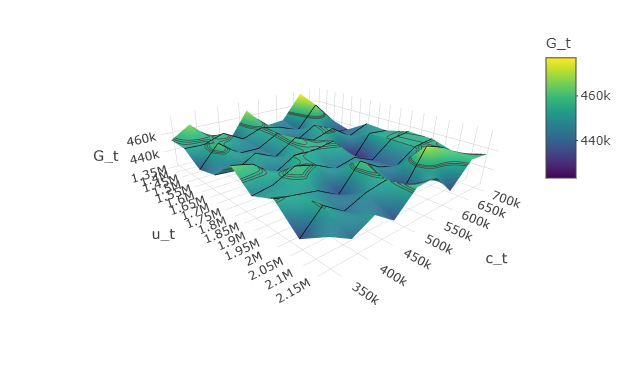
\includegraphics[keepaspectratio]{fig-analisis2pdf.png}}

}

\caption{Superficie del análisis de sensibilidad del modelo
Cramér-Lundberg con variación de parámetros.}

\end{figure}%

Se presenta también el análisis de sensibilidad para \(t = 19\), debido
a que en \(19\) semanas se presenta el caso donde se pueden registrar
ventas por debajo del cero, es decir, casos donde \(G(t)\leq0\).

\begin{Shaded}
\begin{Highlighting}[]
\FunctionTok{library}\NormalTok{(dplyr) }\CommentTok{\# líbreria para poder }
\CommentTok{\# renombrar las cabeceras de los dataframes}

\CommentTok{\# Parámetros}
\FunctionTok{set.seed}\NormalTok{(}\DecValTok{13}\NormalTok{) }\CommentTok{\#semilla fija}
\NormalTok{u }\OtherTok{=} \DecValTok{1759629} \CommentTok{\#surplus(capital inicial de salvamento)}
\CommentTok{\# Es un estimado a partir de la media de las ganancias por semana, }
\CommentTok{\# multiplicado por 10/3, }
\CommentTok{\# siendo una proporción para evitar la ruina}
\CommentTok{\# u (sum(medias))*(10/3)}
\NormalTok{decimal\_c }\OtherTok{=} \FloatTok{0.29}
\NormalTok{c }\OtherTok{=}\NormalTok{decimal\_c}\SpecialCharTok{*}\NormalTok{u }\CommentTok{\#prima de pago cada tiempo t. c = 0.5*u}
\NormalTok{lambda\_Nt }\OtherTok{=} \FloatTok{0.5}
\CommentTok{\#lambda\_Xi = 3}
\NormalTok{t\_final }\OtherTok{=} \DecValTok{19}
\CommentTok{\# S(t) = \textbackslash{}sum\_\{i=1\}\^{}\{N(t)\}X\_i}
\CommentTok{\# donde N(t)\textasciitilde{} Poisson (lambda*t)}
\CommentTok{\# X\_i \textasciitilde{} exponencial (lambda\_Xi)}
\CommentTok{\# CL = REPRESENTA EL MODELO DE CRAMER LUNDBERG}
\CommentTok{\# Simulación de trayectoria de CL\_t, cuando t \textless{} t\_final.}
\NormalTok{trayectoria\_CLt\_post\_pandemia }\OtherTok{\textless{}{-}} \ControlFlowTok{function}\NormalTok{(u, c, lambda\_Nt, t\_final)}
\NormalTok{\{}
\NormalTok{  tiempo }\OtherTok{\textless{}{-}} \FunctionTok{c}\NormalTok{(}\DecValTok{0}\NormalTok{)}
\NormalTok{  Cramer\_trayectoria }\OtherTok{\textless{}{-}} \FunctionTok{c}\NormalTok{(u)}
  \ControlFlowTok{while}\NormalTok{(tiempo[}\FunctionTok{length}\NormalTok{(tiempo)] }\SpecialCharTok{\textless{}}\NormalTok{ t\_final)}
\NormalTok{  \{}
    \CommentTok{\#tiempo\_llegada \textless{}{-} rexp(1, rate = lambda\_Nt)}
\NormalTok{    tiempo\_llegada }\OtherTok{\textless{}{-}}\NormalTok{ (}\DecValTok{1}\NormalTok{)}
\NormalTok{    Y\_i }\OtherTok{\textless{}{-}}\NormalTok{  (}\FunctionTok{rnorm}\NormalTok{(}\DecValTok{1}\NormalTok{, }\AttributeTok{mean =} \FloatTok{101919.050}\NormalTok{ , }\AttributeTok{sd =} \FloatTok{10877.075}\NormalTok{) }\SpecialCharTok{+} 
              \FunctionTok{rnorm}\NormalTok{(}\DecValTok{1}\NormalTok{, }\AttributeTok{mean =}  \FloatTok{39841.721}\NormalTok{ , }\AttributeTok{sd=} \FloatTok{7873.446}\NormalTok{)  }\SpecialCharTok{+}  
              \FunctionTok{rnorm}\NormalTok{(}\DecValTok{1}\NormalTok{, }\AttributeTok{mean =}   \FloatTok{41751.747}\NormalTok{, }\AttributeTok{sd =} \FloatTok{5687.030}\NormalTok{) }\SpecialCharTok{+} 
              \FunctionTok{rnorm}\NormalTok{(}\DecValTok{1}\NormalTok{, }\AttributeTok{mean =}   \FloatTok{43243.143}\NormalTok{, }\AttributeTok{sd =} \FloatTok{10517.841}\NormalTok{)}\SpecialCharTok{+} 
              \FunctionTok{rnorm}\NormalTok{(}\DecValTok{1}\NormalTok{, }\AttributeTok{mean =} \FloatTok{43010.307}\NormalTok{  , }\AttributeTok{sd =} \FloatTok{7741.889}\NormalTok{) }\SpecialCharTok{+} 
              \FunctionTok{rnorm}\NormalTok{(}\DecValTok{1}\NormalTok{, }\AttributeTok{mean =} \FloatTok{61191.300}\NormalTok{  , }\AttributeTok{sd =} \FloatTok{7202.989}\NormalTok{) }\SpecialCharTok{+} 
              \FunctionTok{rnorm}\NormalTok{(}\DecValTok{1}\NormalTok{, }\AttributeTok{mean =}  \FloatTok{85684.058}\NormalTok{ , }\AttributeTok{sd =} \FloatTok{8371.359}\NormalTok{)) }
\NormalTok{    tiempo }\OtherTok{\textless{}{-}} \FunctionTok{c}\NormalTok{(tiempo, tiempo[}\FunctionTok{length}\NormalTok{(tiempo)] }
                \SpecialCharTok{+}\NormalTok{ tiempo\_llegada,tiempo[}\FunctionTok{length}\NormalTok{(tiempo)] }
                \SpecialCharTok{+}\NormalTok{ tiempo\_llegada ) }
\NormalTok{    Cramer\_trayectoria }\OtherTok{\textless{}{-}} \FunctionTok{c}\NormalTok{(Cramer\_trayectoria,}
\NormalTok{                      Cramer\_trayectoria[}\FunctionTok{length}\NormalTok{(Cramer\_trayectoria)]}\SpecialCharTok{{-}} 
\NormalTok{                        c}\SpecialCharTok{*}\NormalTok{tiempo\_llegada, }
\NormalTok{                      Cramer\_trayectoria[}\FunctionTok{length}\NormalTok{(Cramer\_trayectoria)]}\SpecialCharTok{{-}} 
\NormalTok{                       c}\SpecialCharTok{*}\NormalTok{tiempo\_llegada }\SpecialCharTok{+}\NormalTok{  Y\_i )}
    \ControlFlowTok{if}\NormalTok{(Cramer\_trayectoria[}\FunctionTok{length}\NormalTok{(Cramer\_trayectoria)] }\SpecialCharTok{\textless{}} \DecValTok{0}\NormalTok{)}
\NormalTok{    \{}
\NormalTok{      ruina }\OtherTok{=} \DecValTok{1}
\NormalTok{    \}}
    \ControlFlowTok{else}
\NormalTok{    \{}
\NormalTok{      ruina }\OtherTok{=} \DecValTok{0}
\NormalTok{    \}}
\NormalTok{  \}}
\NormalTok{  df\_post\_pandemia}\OtherTok{\textless{}{-}} \FunctionTok{data.frame}\NormalTok{(tiempo, Cramer\_trayectoria)}
\NormalTok{  df\_trayectoria\_post\_pandemia }\OtherTok{\textless{}{-}} \FunctionTok{data.frame}\NormalTok{(df\_post\_pandemia}\SpecialCharTok{\%\textgreater{}\%}
                                  \FunctionTok{rename}\NormalTok{(}\AttributeTok{Tiempo =}\NormalTok{ tiempo, }
                                         \AttributeTok{Ct =}\NormalTok{ Cramer\_trayectoria))}
  \FunctionTok{return}\NormalTok{(df\_trayectoria\_post\_pandemia}\SpecialCharTok{$}\NormalTok{Ct[length}
\NormalTok{                                (df\_trayectoria\_post\_pandemia}\SpecialCharTok{$}\NormalTok{Ct)])}
\NormalTok{\}}

\CommentTok{\# La función generador\_mediana nos calcula la mediana de }
\CommentTok{\# las ganancias finales de 100 trayectorias, }
\CommentTok{\# fijando el u = surplus y el c}
\NormalTok{generador\_mediana\_post\_pandemia}\OtherTok{\textless{}{-}} \ControlFlowTok{function}\NormalTok{(ui,cj)}
\NormalTok{  \{}
\NormalTok{  ganancia\_final\_replicas\_post\_pandemia }\OtherTok{\textless{}{-}} \FunctionTok{replicate}\NormalTok{(}\DecValTok{100}\NormalTok{,}
           \FunctionTok{trayectoria\_CLt\_post\_pandemia}\NormalTok{(u, c,lambda\_Nt, t\_final))}
    \FunctionTok{return}\NormalTok{( }\FunctionTok{median}\NormalTok{(ganancia\_final\_replicas\_post\_pandemia))}
\NormalTok{  \}}
\CommentTok{\# Se crea la rejilla donde se hace el analisis de sensibilidad}
\CommentTok{\# para diferentes valores de u y c}
\NormalTok{grid\_u\_post\_pandemia }\OtherTok{\textless{}{-}} \FunctionTok{seq}\NormalTok{(}\AttributeTok{from =}\NormalTok{ (u}\DecValTok{{-}100000}\SpecialCharTok{*}\DecValTok{4}\NormalTok{), }
                            \AttributeTok{to =}\NormalTok{ (u}\SpecialCharTok{+}\DecValTok{100000}\SpecialCharTok{*}\DecValTok{4}\NormalTok{), }
                            \AttributeTok{by =} \DecValTok{100000}\NormalTok{)}
\NormalTok{grid\_c\_post\_pandemia }\OtherTok{\textless{}{-}} \FunctionTok{seq}\NormalTok{(}\AttributeTok{from =}\NormalTok{ (decimal\_c}\FloatTok{{-}0.01}\SpecialCharTok{*}\DecValTok{4}\NormalTok{), }
                            \AttributeTok{to =}\NormalTok{ (decimal\_c}\FloatTok{+0.01}\SpecialCharTok{*}\DecValTok{4}\NormalTok{), }
                            \AttributeTok{by =} \FloatTok{0.01}\NormalTok{)}
\NormalTok{u\_t }\OtherTok{\textless{}{-}}\NormalTok{ grid\_u\_post\_pandemia}
\NormalTok{matriz\_mediana\_post\_pandemia }\OtherTok{\textless{}{-}} \FunctionTok{matrix}\NormalTok{(}\FunctionTok{rep}\NormalTok{(}\DecValTok{0}\NormalTok{, }
      \FunctionTok{length}\NormalTok{(grid\_u\_post\_pandemia)}\SpecialCharTok{*}\FunctionTok{length}\NormalTok{(grid\_c\_post\_pandemia)),}
      \AttributeTok{nrow=} \FunctionTok{length}\NormalTok{(grid\_u\_post\_pandemia), }
      \AttributeTok{ncol=} \FunctionTok{length}\NormalTok{(grid\_c\_post\_pandemia))}

\NormalTok{G\_t }\OtherTok{\textless{}{-}}\NormalTok{ matriz\_mediana\_post\_pandemia}

\ControlFlowTok{for}\NormalTok{ (i }\ControlFlowTok{in} \DecValTok{1}\SpecialCharTok{:}\FunctionTok{length}\NormalTok{(u\_t)) }
\NormalTok{\{}
  \ControlFlowTok{for}\NormalTok{ (j }\ControlFlowTok{in} \DecValTok{1}\SpecialCharTok{:}\FunctionTok{length}\NormalTok{(grid\_c\_post\_pandemia)) }
\NormalTok{  \{}
\NormalTok{    G\_t[i,j] }\OtherTok{\textless{}{-}} \FunctionTok{generador\_mediana\_post\_pandemia}\NormalTok{(u\_t[i], }
\NormalTok{                                  grid\_c\_post\_pandemia[j]}\SpecialCharTok{*}\NormalTok{u\_t[i])}
\NormalTok{  \}}
\NormalTok{\} }

\CommentTok{\#Grafica del ánalisis de sensibilidad}

\NormalTok{c\_t }\OtherTok{\textless{}{-}}\NormalTok{ grid\_u\_post\_pandemia}\SpecialCharTok{*}\NormalTok{grid\_c\_post\_pandemia}

\NormalTok{z1}\OtherTok{\textless{}{-}} \FunctionTok{matrix}\NormalTok{(}\FunctionTok{rep}\NormalTok{(}\DecValTok{0}\NormalTok{,}
\FunctionTok{length}\NormalTok{(grid\_u\_post\_pandemia)}\SpecialCharTok{*}\FunctionTok{length}\NormalTok{(grid\_c\_post\_pandemia)), }\AttributeTok{nrow=}
\FunctionTok{length}\NormalTok{(grid\_u\_post\_pandemia), }\AttributeTok{ncol=} \FunctionTok{length}\NormalTok{(grid\_c\_post\_pandemia))}

\NormalTok{z2}\OtherTok{\textless{}{-}} \FunctionTok{matrix}\NormalTok{(}\FunctionTok{rep}\NormalTok{(u,}
\FunctionTok{length}\NormalTok{(grid\_u\_post\_pandemia)}\SpecialCharTok{*}\FunctionTok{length}\NormalTok{(grid\_c\_post\_pandemia)), }\AttributeTok{nrow=}
\FunctionTok{length}\NormalTok{(grid\_u\_post\_pandemia), }\AttributeTok{ncol=} \FunctionTok{length}\NormalTok{(grid\_c\_post\_pandemia))}

\NormalTok{fig3 }\OtherTok{\textless{}{-}} \FunctionTok{plot\_ly}\NormalTok{(}
  \AttributeTok{type =} \StringTok{\textquotesingle{}surface\textquotesingle{}}\NormalTok{,}
  \AttributeTok{contours =} \FunctionTok{list}\NormalTok{(}
    \AttributeTok{x =} \FunctionTok{list}\NormalTok{(}\AttributeTok{show =} \ConstantTok{TRUE}\NormalTok{, }\AttributeTok{start =}\NormalTok{ u\_t[}\DecValTok{1}\NormalTok{], }\AttributeTok{end =}
\NormalTok{u\_t[}\FunctionTok{length}\NormalTok{(u\_t)], }\AttributeTok{size =}\DecValTok{100000}\NormalTok{ ,}
\AttributeTok{color =} \StringTok{\textquotesingle{}black\textquotesingle{}}\NormalTok{),}
    \AttributeTok{z =} \FunctionTok{list}\NormalTok{(}\AttributeTok{show =} \ConstantTok{TRUE}\NormalTok{, }\AttributeTok{start =}\NormalTok{ G\_t[}\DecValTok{1}\NormalTok{], }
             \AttributeTok{end =}\NormalTok{ G\_t[}\FunctionTok{length}\NormalTok{(G\_t)], }\AttributeTok{size =}\FloatTok{0.01}\SpecialCharTok{*}\DecValTok{100000}\NormalTok{ , }
             \AttributeTok{color =} \StringTok{\textquotesingle{}white\textquotesingle{}}\NormalTok{)),}
  \AttributeTok{x =} \SpecialCharTok{\textasciitilde{}}\NormalTok{u\_t,}
  \AttributeTok{y =} \SpecialCharTok{\textasciitilde{}}\NormalTok{c\_t,}
  \AttributeTok{z =} \SpecialCharTok{\textasciitilde{}}\NormalTok{G\_t)}

\NormalTok{fig3 }\OtherTok{\textless{}{-}}\NormalTok{ fig3}\SpecialCharTok{\%\textgreater{}\%} \FunctionTok{add\_surface}\NormalTok{(}
  \AttributeTok{type =} \StringTok{\textquotesingle{}surface\textquotesingle{}}\NormalTok{,}
  \AttributeTok{contours =} \FunctionTok{list}\NormalTok{(}
    \AttributeTok{x =} \FunctionTok{list}\NormalTok{(}\AttributeTok{show =} \ConstantTok{TRUE}\NormalTok{, }\AttributeTok{start =}\NormalTok{ u\_t[}\DecValTok{1}\NormalTok{], }
             \AttributeTok{end =}\NormalTok{ u\_t[}\FunctionTok{length}\NormalTok{(u\_t)], }\AttributeTok{size =}\DecValTok{100000}\NormalTok{ ,}
             \AttributeTok{color =} \StringTok{\textquotesingle{}black\textquotesingle{}}\NormalTok{),}
    \AttributeTok{y =} \FunctionTok{list}\NormalTok{(}\AttributeTok{show =} \ConstantTok{TRUE}\NormalTok{, }\AttributeTok{start =}\NormalTok{ c\_t[}\DecValTok{1}\NormalTok{], }
             \AttributeTok{end =}\NormalTok{ c\_t[}\FunctionTok{length}\NormalTok{(c\_t)], }
             \AttributeTok{size =} \FloatTok{0.01}\SpecialCharTok{*}\DecValTok{100000}\NormalTok{ , }\AttributeTok{color =} \StringTok{\textquotesingle{}red\textquotesingle{}}\NormalTok{)),}
  \AttributeTok{x =} \SpecialCharTok{\textasciitilde{}}\NormalTok{u\_t,}
  \AttributeTok{y =} \SpecialCharTok{\textasciitilde{}}\NormalTok{c\_t,}
  \AttributeTok{z =} \SpecialCharTok{\textasciitilde{}}\NormalTok{z1)}

\NormalTok{fig3 }\OtherTok{\textless{}{-}}\NormalTok{ fig3 }\SpecialCharTok{\%\textgreater{}\%} \FunctionTok{layout}\NormalTok{(}
  \AttributeTok{scene =} \FunctionTok{list}\NormalTok{(}
    \AttributeTok{xaxis =} \FunctionTok{list}\NormalTok{(}\AttributeTok{nticks =} \DecValTok{20}\NormalTok{),}
    \AttributeTok{zaxis =} \FunctionTok{list}\NormalTok{(}\AttributeTok{nticks =} \DecValTok{4}\NormalTok{),}
    \AttributeTok{camera =} \FunctionTok{list}\NormalTok{(}\AttributeTok{eye =} \FunctionTok{list}\NormalTok{(}\AttributeTok{x =} \DecValTok{0}\NormalTok{, }\AttributeTok{y =} \SpecialCharTok{{-}}\DecValTok{1}\NormalTok{, }\AttributeTok{z =} \DecValTok{1}\NormalTok{)),}
    \AttributeTok{aspectratio =} \FunctionTok{list}\NormalTok{(}\AttributeTok{x =}\NormalTok{ .}\DecValTok{9}\NormalTok{, }\AttributeTok{y =}\NormalTok{ .}\DecValTok{8}\NormalTok{, }\AttributeTok{z =} \FloatTok{0.2}\NormalTok{)))}


\NormalTok{fig3}
\end{Highlighting}
\end{Shaded}

\begin{figure}[H]

{\centering 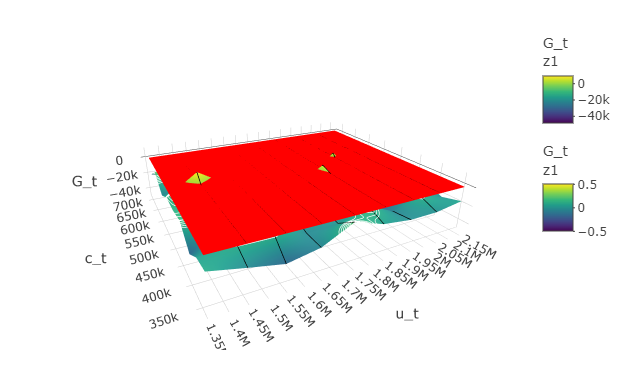
\includegraphics[width=6.25in,height=\textheight,keepaspectratio]{fig-analisis3pdf.png}

}

\caption{Superficie del eje cero y de los resultados post pandemicos del
análisis de sensibilidad del modelo Cramér-Lundberg variando los
parámetros.}

\end{figure}%

\section{Análisis de resultados y
recomendaciones.}\label{anuxe1lisis-de-resultados-y-recomendaciones.}

Con los datos registrados de \(90\) semanas antes de pandemia en el
modelo modificado (Ecuación~\ref{eq-4.1pdf}) se obtiene un crecimiento
positivo de las ganancias simuladas, en particular mayor que el capital
inicial, es decir la probabilidad del evento donde \(G(t)\geq u\) es
positiva, con \(t=90\), como se puede observar en la imagen
(Figura~\ref{fig-fig-trayectoriapdf}), por lo que en el intervalo de
tiempo en el que se estudia la empresa generaría siempre ganancias
positivas y se lograría suplir la deuda e incluso pensar en implementar
más equipos inmobiliarios.

Mientras que después de la pandemia, se puede argumentar con base en las
observaciones de las \(14\) semanas de las ventas registradas, usando
los mismos parámetros obtenidos para los datos antes de la pandemia
implementados, las ganancias son bajas como se muestra en la imagen
(Figura~\ref{fig-fig-trayectoria2pdf}). Aquí se observa que la
simulación de las ganancias son menores que el capital inicial y al dar
seguimiento en el intervalo de tiempo con los datos registrados después
de pandemia hasta la semana \(17\), se observa que las ganancias son
menores que cero, por lo que se puede concluir que se llega a una ruina
total, como se muestra el caso en la imagen
(Figura~\ref{fig-fig-trayectoria3pdf}).

Analizando el caso en el que se modifica los parámetros de los costos
del modelo (Ecuación~\ref{eq-4.1pdf}), se concluye que al calibrar el
parámetro \(c\), este se puede reducir a un \(17 \%\) para cuando
\(t=14\), es decir, al final de la semana \(14\) puede evitarse la
perdida total de las ganancias que son mayores que el capital inicial,
como se observa en la figura (Figura~\ref{fig-fig-trayectoria4pdf}).

Como \(c\), es el parámetro de los pagos que incluye el pago de la
adquisición de la franquicia, compras de equipos inmobiliarios, pagos de
empleados y préstamos, el anterior análisis quiere decir que se necesita
un recorte de personal del \(17 \%\) como mínimo y una reestructuración
financiera del capital pendiente por pagar, haciendo los pagos más
pequeños a un tiempo extendido, con el fin de la funcionalidad del
negocio durante este proceso pandemico y evitar el cierre de quiebra.

\bookmarksetup{startatroot}

\chapter{Conclusiones}\label{conclusiones}

El presente trabajo de tesis, titulado ``Estudio del impacto de la
pandemia en un establecimiento de comida rápida: Análisis y estimación
de parámetros para el modelo modificado de Cramér-Lundberg'', permitió
abordar un análisis detallado de los efectos de la pandemia sobre la
operación, sostenibilidad y riesgos financieros en este tipo de
negocios, utilizando un marco matemático basado en el modelo modificado
de Cramér-Lundberg.

En primer lugar, los resultados obtenidos evidencian que la pandemia
tuvo un impacto significativo en las dinámicas operativas y financieras
del establecimiento. Factores como la reducción en el número de
clientes, la implementación de medidas de distanciamiento social y los
cambios en los hábitos de consumo fueron determinantes en la disminución
de ingresos. Este fenómeno obligó al establecimiento a redefinir
estrategias operativas, incluyendo la digitalización de sus servicios,
la incorporación de entregas a domicilio y ajustes en su estructura de
costos.

A través del modelo de Cramér-Lundberg modificado, se logró estimar y
analizar los parámetros clave, como las tasas de llegada de pedidos, los
montos promedio de gasto por cliente y las pérdidas por interrupciones
de operación. Los resultados sugieren que, si bien el establecimiento
experimentó un alto riesgo de insolvencia en los meses más críticos de
la pandemia, las estrategias de adaptación implementadas contribuyeron
significativamente a reducir este riesgo con el tiempo. En particular,
el enfoque en la diversificación de los canales de venta y la
optimización de costos demostró ser esencial para la supervivencia del
negocio.

Además, este estudio destaca la importancia de incorporar modelos
probabilísticos como herramientas para la toma de decisiones
estratégicas en contextos de incertidumbre. La flexibilidad del modelo
modificado permitió capturar las particularidades del contexto
pandémico, ofreciendo una visión integral de los riesgos financieros
asociados. Esto pone de manifiesto la relevancia de utilizar
herramientas cuantitativas no solo para evaluar riesgos sino también
para proyectar escenarios futuros y evaluar el impacto de decisiones
estratégicas.

En términos prácticos, las conclusiones del estudio ofrecen
recomendaciones aplicables no solo para el establecimiento analizado,
sino también para otros negocios similares que enfrenten condiciones de
incertidumbre y crisis. La capacidad de adaptarse a cambios en el
entorno externo y de incorporar herramientas analíticas para una gestión
proactiva de riesgos resulta fundamental en un mercado altamente
competitivo.

Finalmente, este trabajo abre la puerta para investigaciones futuras,
tales como la aplicación del modelo en otros sectores afectados por la
pandemia, el análisis de impactos a largo plazo y la exploración de
estrategias de recuperación más eficientes. Se concluye que la
combinación de modelos matemáticos con estudios de caso específicos
proporciona una base sólida para enfrentar desafíos complejos,
contribuyendo tanto al ámbito académico como al sector empresarial.

\bookmarksetup{startatroot}

\chapter{Sugerencias y/o recomendaciones y/o
propuestas.}\label{sugerencias-yo-recomendaciones-yo-propuestas.}

\phantomsection\label{text-align:justify}
El modelo de Cramér-Lundberg es un modelo clásico en teoría del riesgo
utilizado para modelar la evolución temporal de las reservas de una
compañía de seguros.

Aunque el modelo de Cramér-Lundberg no es en sí un problema de
optimización, se pueden desarrollar problemas de optimización lineal
relacionados con ciertos aspectos del modelo implementando cadenas de
suministros, en el cual se requiere optimizar los costos, garantizar la
calidad del producto y satisfacer la demanda a tiempo, presentado así en
algunos proyectos y tomando de referencias
(\textcite{martinez2021evaluacion}, \textcite{sanchez2021retos})

Estos pueden incluir:

\begin{enumerate}
\def\labelenumi{\arabic{enumi}.}
\item
  Optimización de ganancias : Un objetivo podría ser maximizar las
  ganancias de la empresa mientras se minimiza la probabilidad de ruina
  o se mantiene una probabilidad aceptable de no ruina. En la
  optimización de las ganancias ciertas restricciones pueden ser
  formuladas como un problema de programación lineal si las relaciones
  son lineales (como el cálculo de ingresos esperados versus
  reclamaciones).
\item
  Algunos de los parámetros del modelo, como la cantidad de recursos
  asignados a publicidad, costos variables por servicio (como personal o
  insumos), o estrategias para mitigar las pérdidas, pueden ser
  convertidos en variables de decisión en un problema de optimización.

  Si los parámetros se pueden expresar como relaciones lineales, se
  puede definir una función objetivo que maximice las ganancias o
  minimice las pérdidas del establecimiento durante la pandemia.
\end{enumerate}

Pudiendo así implementarlas en distintos problemas o estrategias que se
presenten como:

\begin{itemize}
\item
  Reducir el horario de atención.
\item
  Invertir en publicidad digital.
\item
  Ampliar el menú con opciones para llevar.
\end{itemize}

En conclusión, generalmente aunque el modelo de Cramér-Lundberg está
basado en un enfoque estocástico, ciertos aspectos del problema pueden
ser reformulados como un problema de optimización lineal, especialmente
si el enfoque se centra en la gestión de recursos y la maximización de
las ganancias bajo restricciones.

\bookmarksetup{startatroot}

\chapter*{Lista de obras consultadas}\label{lista-de-obras-consultadas}
\addcontentsline{toc}{chapter}{Lista de obras consultadas}

\markboth{Lista de obras consultadas}{Lista de obras consultadas}

\printbibliography[heading=none]





\end{document}
